\documentclass{article}
\usepackage[utf8]{inputenc}
\usepackage[margin=0.70in]{geometry}
\usepackage{hyperref}
\usepackage{graphicx}
\usepackage{authblk}
\usepackage{subfig}
\usepackage{indentfirst}

\title{Project 3: DNN Hyperparameter Optimization via NNI}
\author{Oliver Fowler}
\author{Brian Park}
\affil{North Carolina State University, Computer Science 591/791-025}
\date{October 2022}

\begin{document}
\maketitle


% Go through the Hyper-parameter Optimization chapters in the User Guide and Reference of NNI. Those chapters are marked in red boxes in the attached "hpo.pdf" screenshot. 

% Apply at least three of the hyper-parameter tuners in the list of NNI HPO to one of the example models in this repository. (Hint: this model can be trained quickly; but you don't have to use this one. ) You can decide what hyperparameters to tune, which can be learning rate, batch size, or even some hyperparameter you add into the model. There should be at least two hyperparameters to tune.
% In the application of an HPO method, try at least two different configurations of the HPO to see the differences in the tuning speed and tuning result.

\section{HPO Methods}
%(1) What HPO tuners you have applied to which DNN model.

We use NNI to do hyperparameter optimization \cite{nni}. We tried multiple tuners such as TPE, Evolution, and Hyperband \cite{tpe, evolution, hyperband}. We use a simple shallow multi-layer perceptron on MNIST Fashion dataset. This was an example provided by PyTorch. We chose this due to time constraints as we had issues with setting up and allocating nodes on ARC cluster. Other classes were also doing compute intensive assignments, making it difficult to train a more complex model. When we had time left over after doing the required portions, we used a more resource demanding DNN, VGG-19 on CIFAR-10 \cite{vgg}.


\section{HPO and Hardware Configurations}
%(2) What configurations did you try on each HPO tuner, and what machine(s) you have used, including the CPU and GPU models of the machine(s). 

\subsection{HPO Configurations}
For the tuner configurations we used TPE, Evolution, and Hyperband \cite{tpe, evolution, hyperband}. For hyperparamters to tune, we set the \verb|optimize| mode to \verb|maximize| and let the tuner handle the rest. We set parameters for the learning rate and momentum. For the secondary configuration, we also experimented and treated the number of features and batch size as hyperparameters. Varying both the feature size and batch size will give us a sense of speed. Smaller batches will generally lead to slower training times but higher accuracy, while larger batches will be able to exploit parallelism to get faster training times, but lower accuracy.

For VGG-19, we repeated the configurations, but number of features is not implemented since we loaded a premade model from PyTorch.

The configurations is as follows:
\begin{itemize}
    \item Learning Rate: Log uniformly sampled between $0.0001, 0.1$
    \item Momentum: Uniformly sampled between $0, 1$
    \item Features: $128, 256, 512, 1024$
    \item Batch Size: $1, 4, 32, 64, 128, 256$
\end{itemize}

\subsection{Hardware Configurations}
We had difficulties running the hyperparameter tuner experiments successfully on the ARC cluster \cite{arc}. We were fortunate enough to get access to the PSC's bridges-2 supercomputer, which uses 8 NVIDIA V100 SXM2 per node, part of a DGX system \cite{v100, bridges-2}. The DGX system uses has two Intel(R) Xeon(R) Gold 6148 CPU @ 2.40GHz CPUs. When allocated via the name \verb|GPU-Shared|, we will only connect to 1 CPU and 1 GPU, as only 4 GPUs are connected via PCIe per CPU node. We use a single GPU, as we're not aware if NNI can utilize multiple GPU in a intra-node setting. Oliver used his RTX 3080 Ti and Brian was able to use his M1 Mac to do the hyperparameter search for each configuration and tuner concurrently. Once we reached an agreement that our code was working and correct for a few configurations, we executed all the configurations on the bridges-2 system for consistency on the V100 GPU in a single batch. 

\section{Experimental Results}
%(3) What results you have obtained, including the hyperparameters the tuner finds at the end and the impact (e.g., the accuracy and speed of the resulting model), and also your explanations of the reasons for the differences in the results from the different methods and configurations.
First, we did hyperparemter tuning on the MNIST Fashion dataset \cite{fashion-mnist}. It's a grayscale image dataset with 10 labels. Dataset contains 60,000 images for the training set and 10,000 images for the test set. We initially wanted to use CIFAR-10, but realized that would make the hyperparameter optimization very slow and resource intensive, since it requires deeper networks \cite{cifar10}. As oppposed to the MNIST digit dataset, we chose MNIST fashion as it seems quick to train, yet slightly difficult to optimize compared against the digit dataset. We wanted to see interesting results. Running locally on our laptops took around 1 hour for one hyperparameter tuning experiment to end. On the V100, it took just over an hour to run \textit{all 6} configurations. We did 20 trials for each experiment with concurrency set to 20. We wanted to achieve peak utilization to efficiently use the GPUs, but weren't sure what a right number would be for concurrency. We tried 10 and 100, but found that 100 will hit OOM and fail a lot of experiments. So we chose 20 as a safe choice. Table \ref{table:summary} shows a summary of our results.

%Experiment IDs:
% MLP with no batch
% i5crdozm
% c6fjwn74
% 4mixwfhs

% MLP with batching
% z7shknrj
% 41bvtiok
% srfpgh3w

% VGG-19
% oamshqwn
% sct3jm0z

\begin{table}[ht]
\caption{Hyperparameter Summary for MLP on Fashion MNIST} % title of Table
\centering % used for centering table
\begin{tabular}{c c c c c c c c } % centered columns (8 columns)
\hline\hline %inserts double horizontal lines
HPO Tuner & Trial & Validation Accuracy & Learning Rate & Momentum & Batch Size & Feature Size \\ [0.5ex] % inserts table
%heading
\hline % inserts single horizontal line
TPE                  & 9  & 88.26\% & 0.0763 & 0.5338 & -- & --  \\
Evolution            & 13 & 87.98\% & 0.0269 & 0.5765 & -- & --  \\
Hyperband            & 2  & 88.33\% & 0.0855 & 0.6975 & -- & --  \\
TPE with batch       & 6  & 88.26\% & 0.0476 & 0.4535 & 64 & 512 \\
Evolution with batch & 2  & 87.98\% & 0.0794 & 0.4306 & 32 & 512 \\
Hyperband with batch & 6  & 88.14\% & 0.0244 & 0.7010 & 32 & 512 \\
[1ex] % [1ex] adds vertical space
\hline %inserts single line
\end{tabular}
\label{table:summary} % is used to refer this table in the text
\end{table}


\subsection{MLP HPO Experiments with Learning Rate and Momentum}
Figure \ref{fig:mlp-tpe} shows the result of the MLP with TPE. We observe that Trial 9 has the most optimal parameters with a validation accuracy of 88.26\%. The optimal parameters for this trial are a learning rate of $0.0763$ and a momentum of $0.5338$. We also observe that the duration for all trials is about 5 minutes.

\begin{figure}
    \centerline{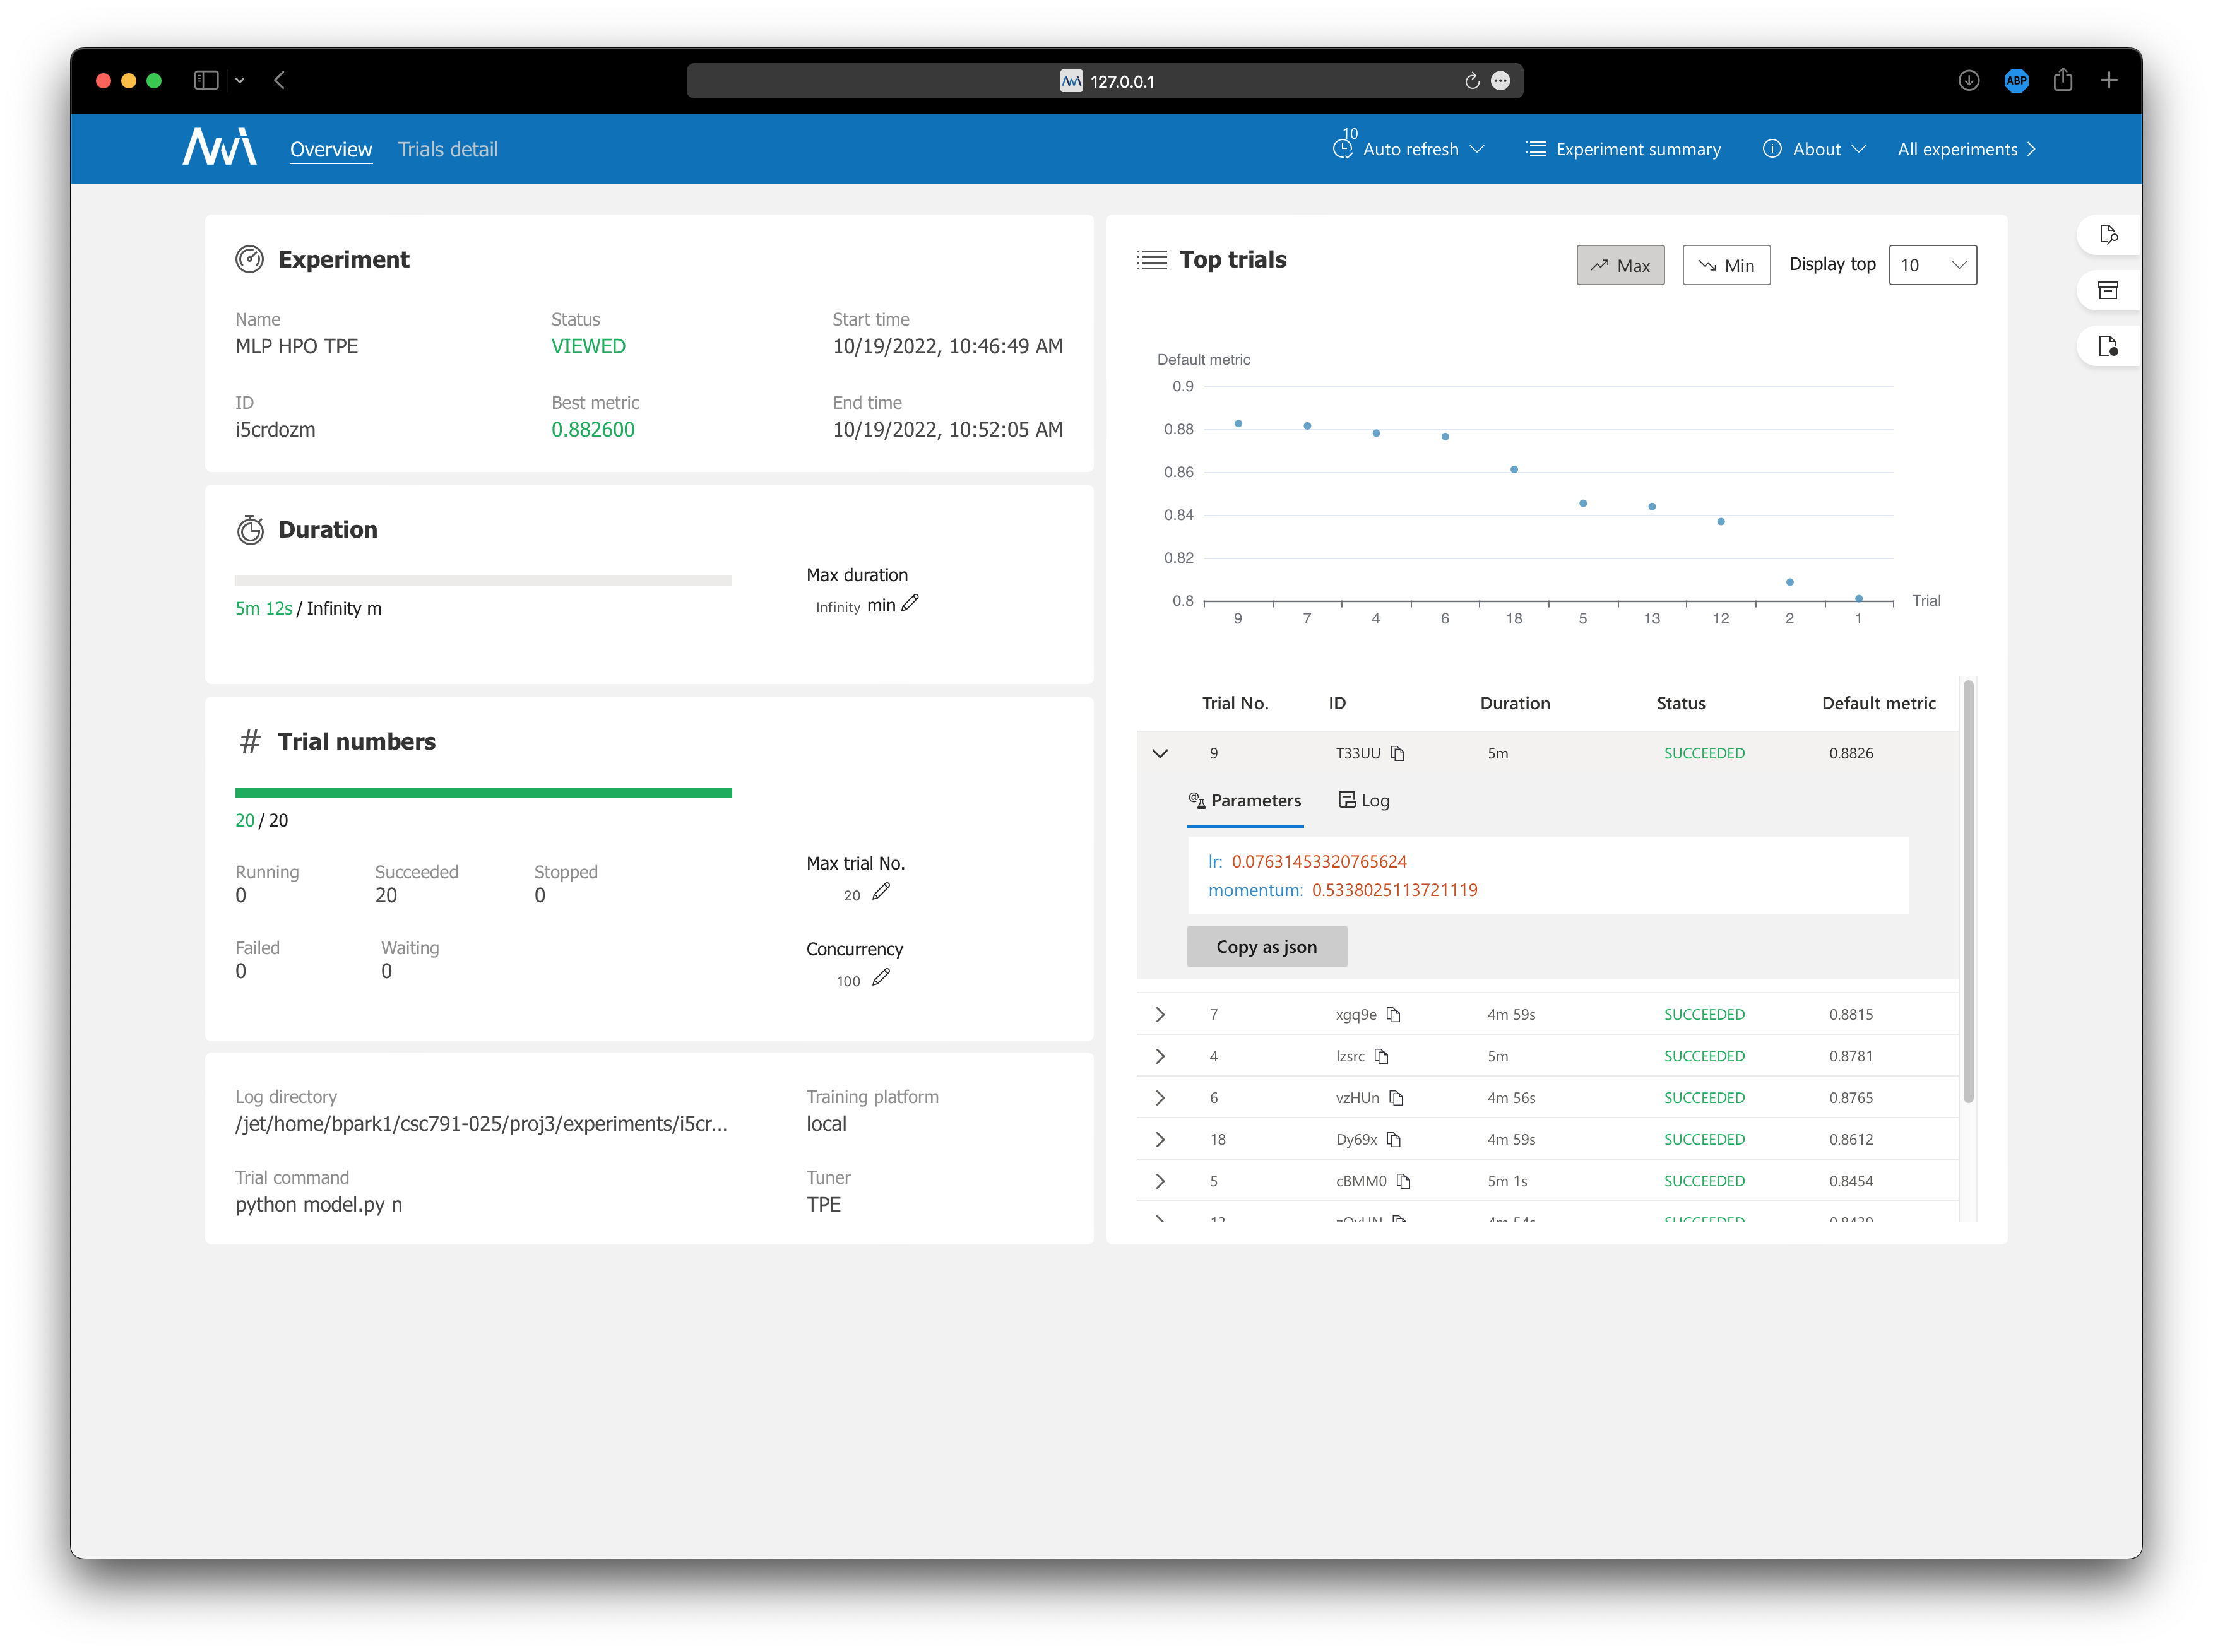
\includegraphics[width=3.5in]{../proj3/figures/mlp_tpe_overview.png}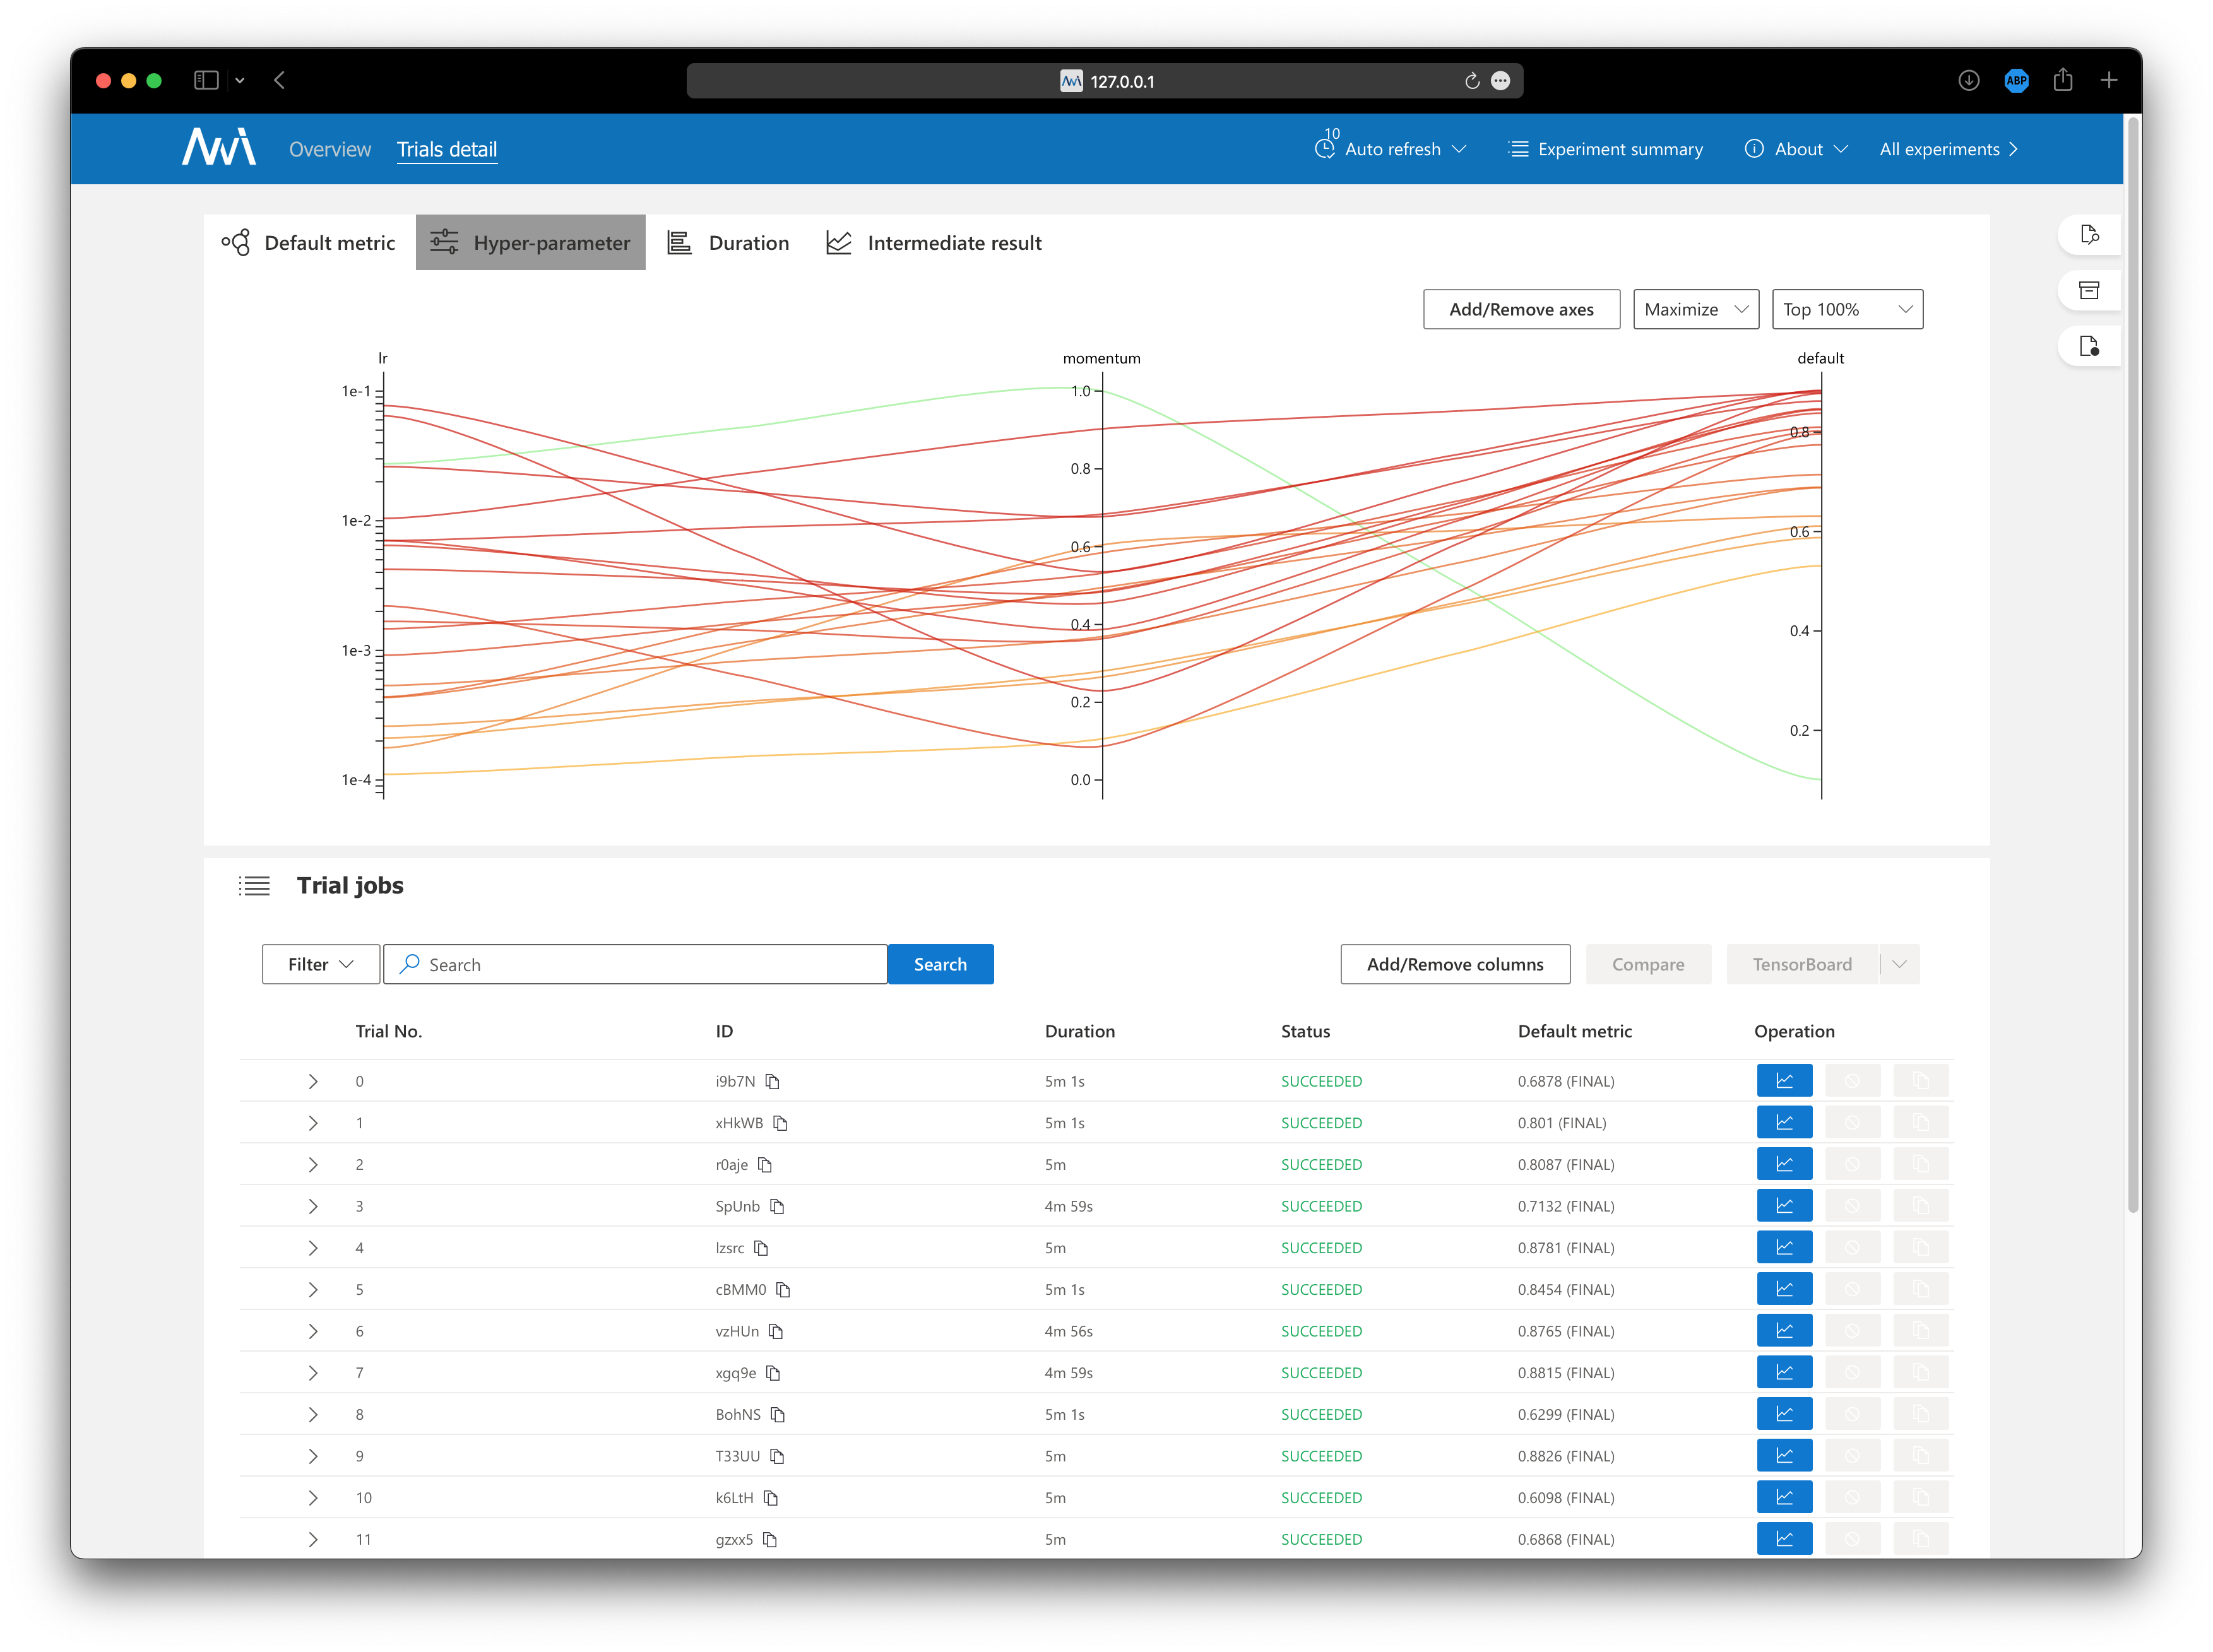
\includegraphics[width=3.5in]{../proj3/figures/mlp_tpe_hyperparameter.png}}
    \centerline{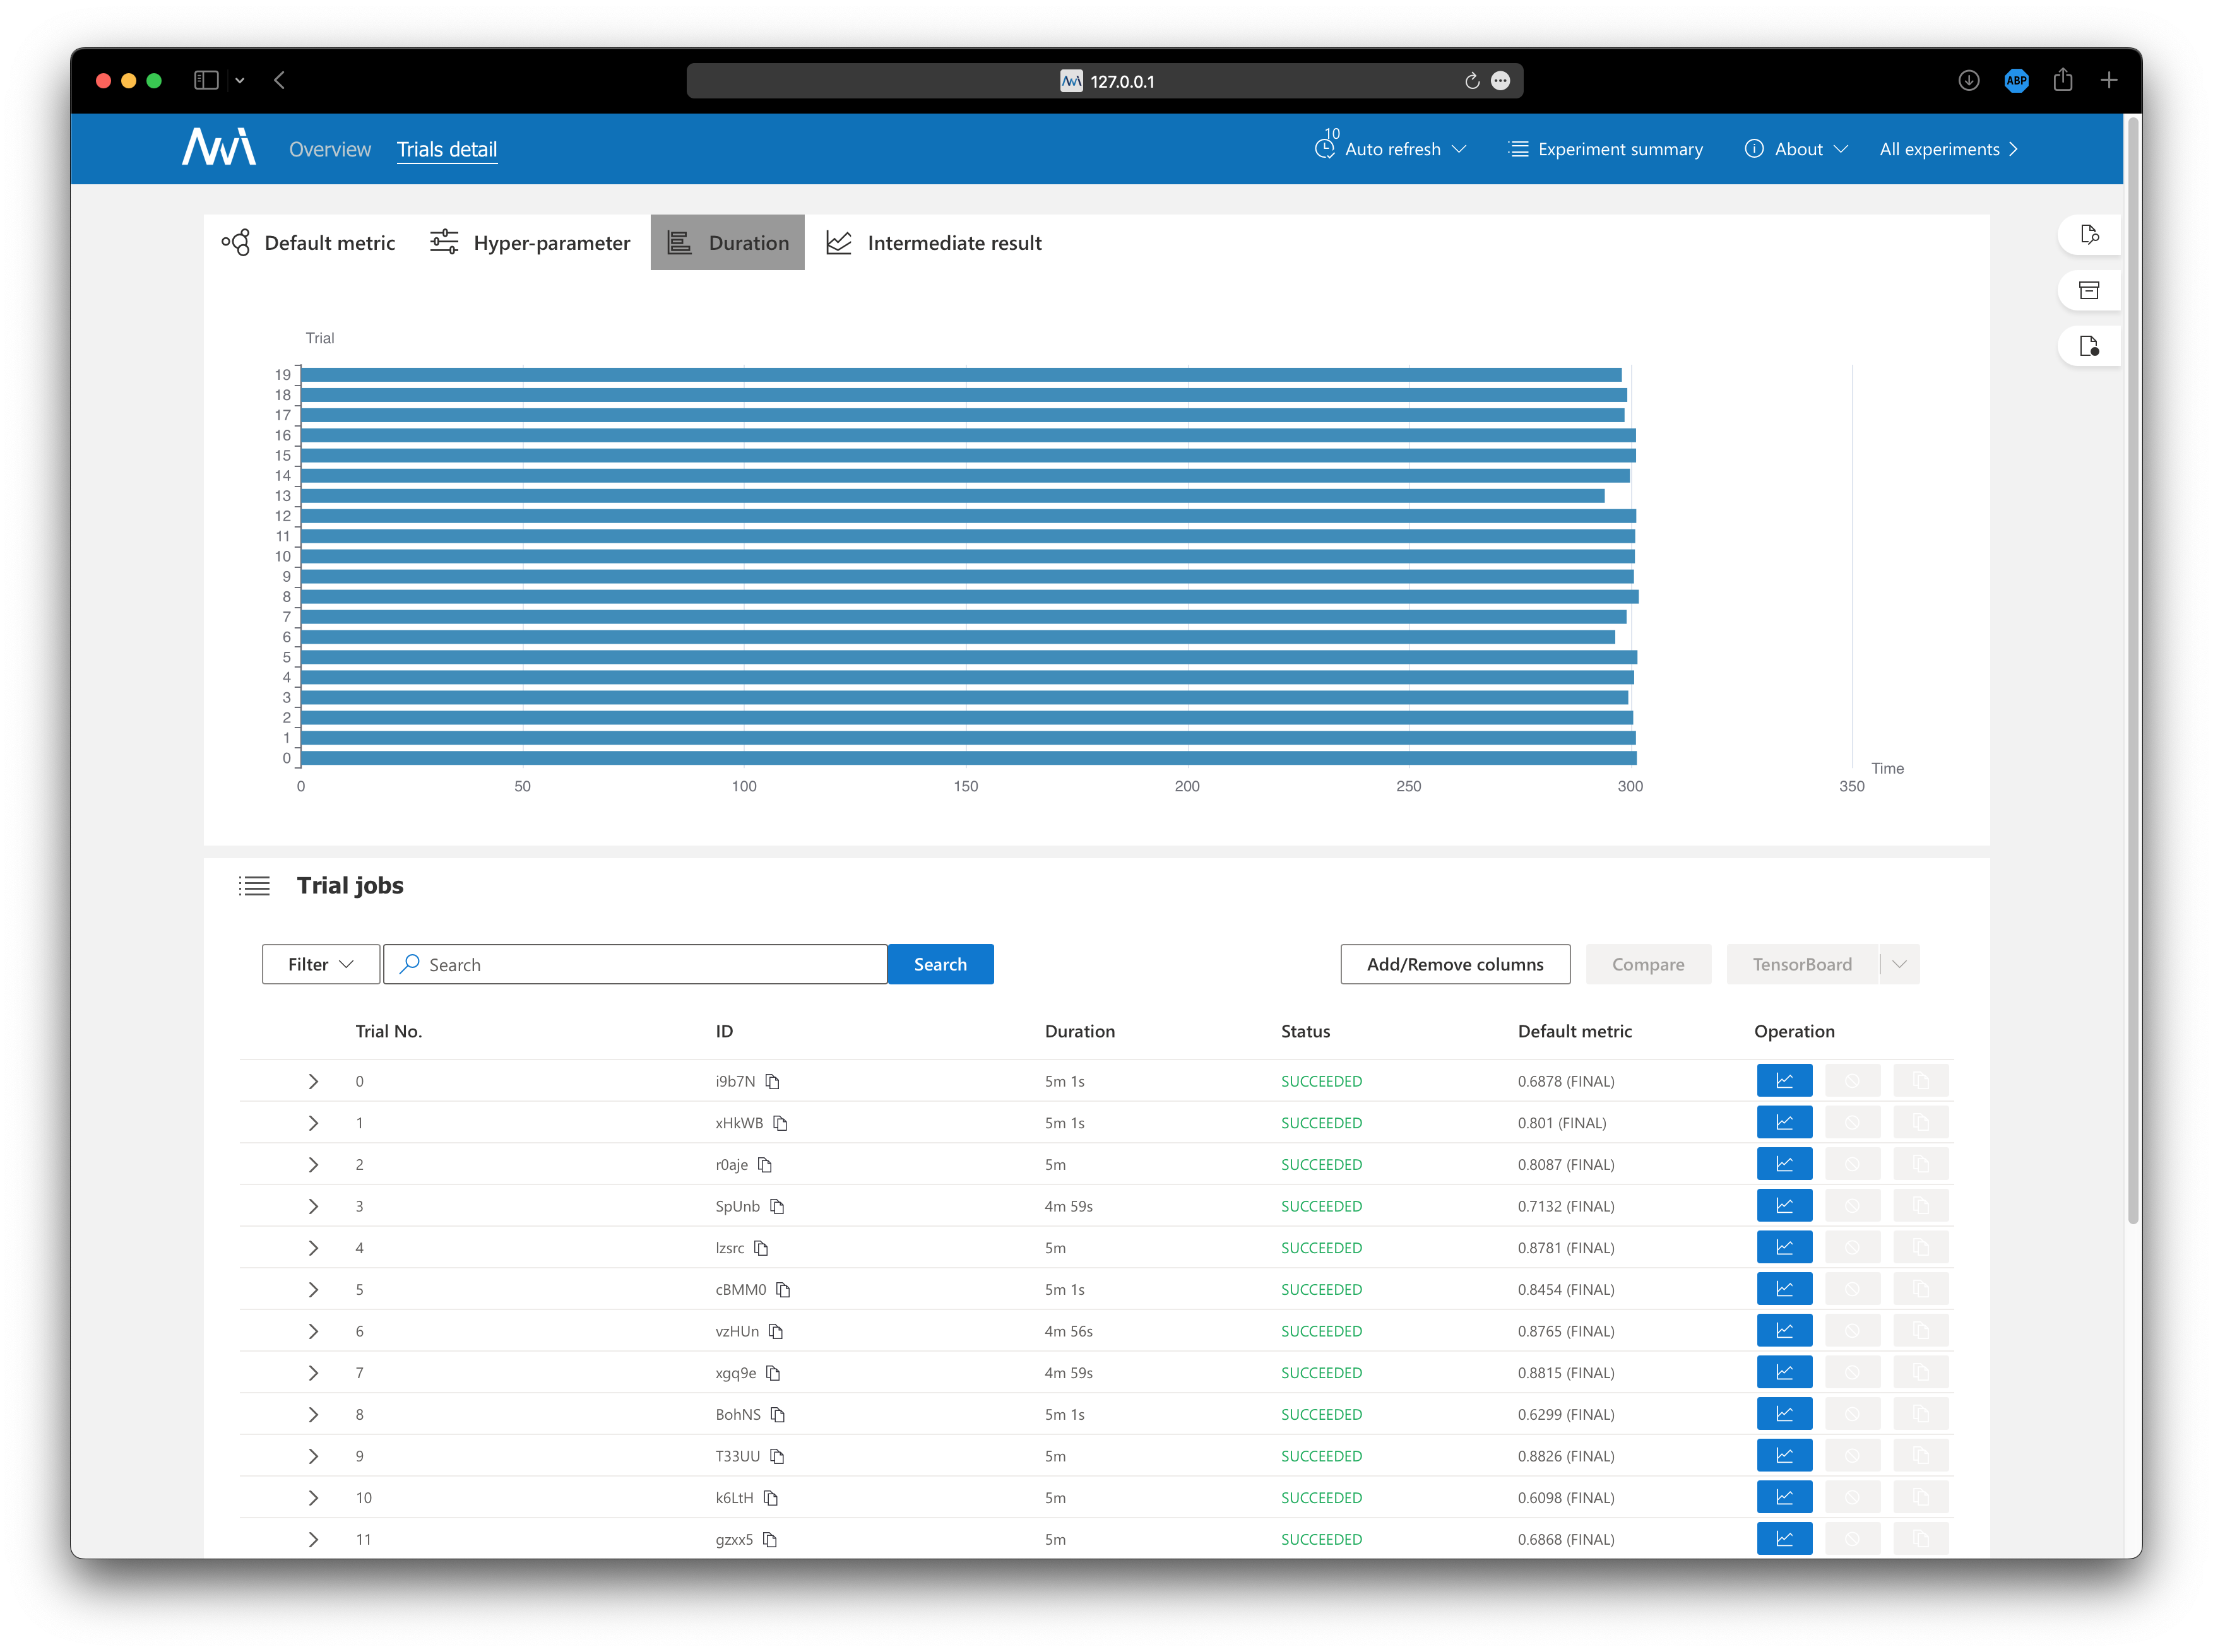
\includegraphics[width=3.5in]{../proj3/figures/mlp_tpe_latency.png}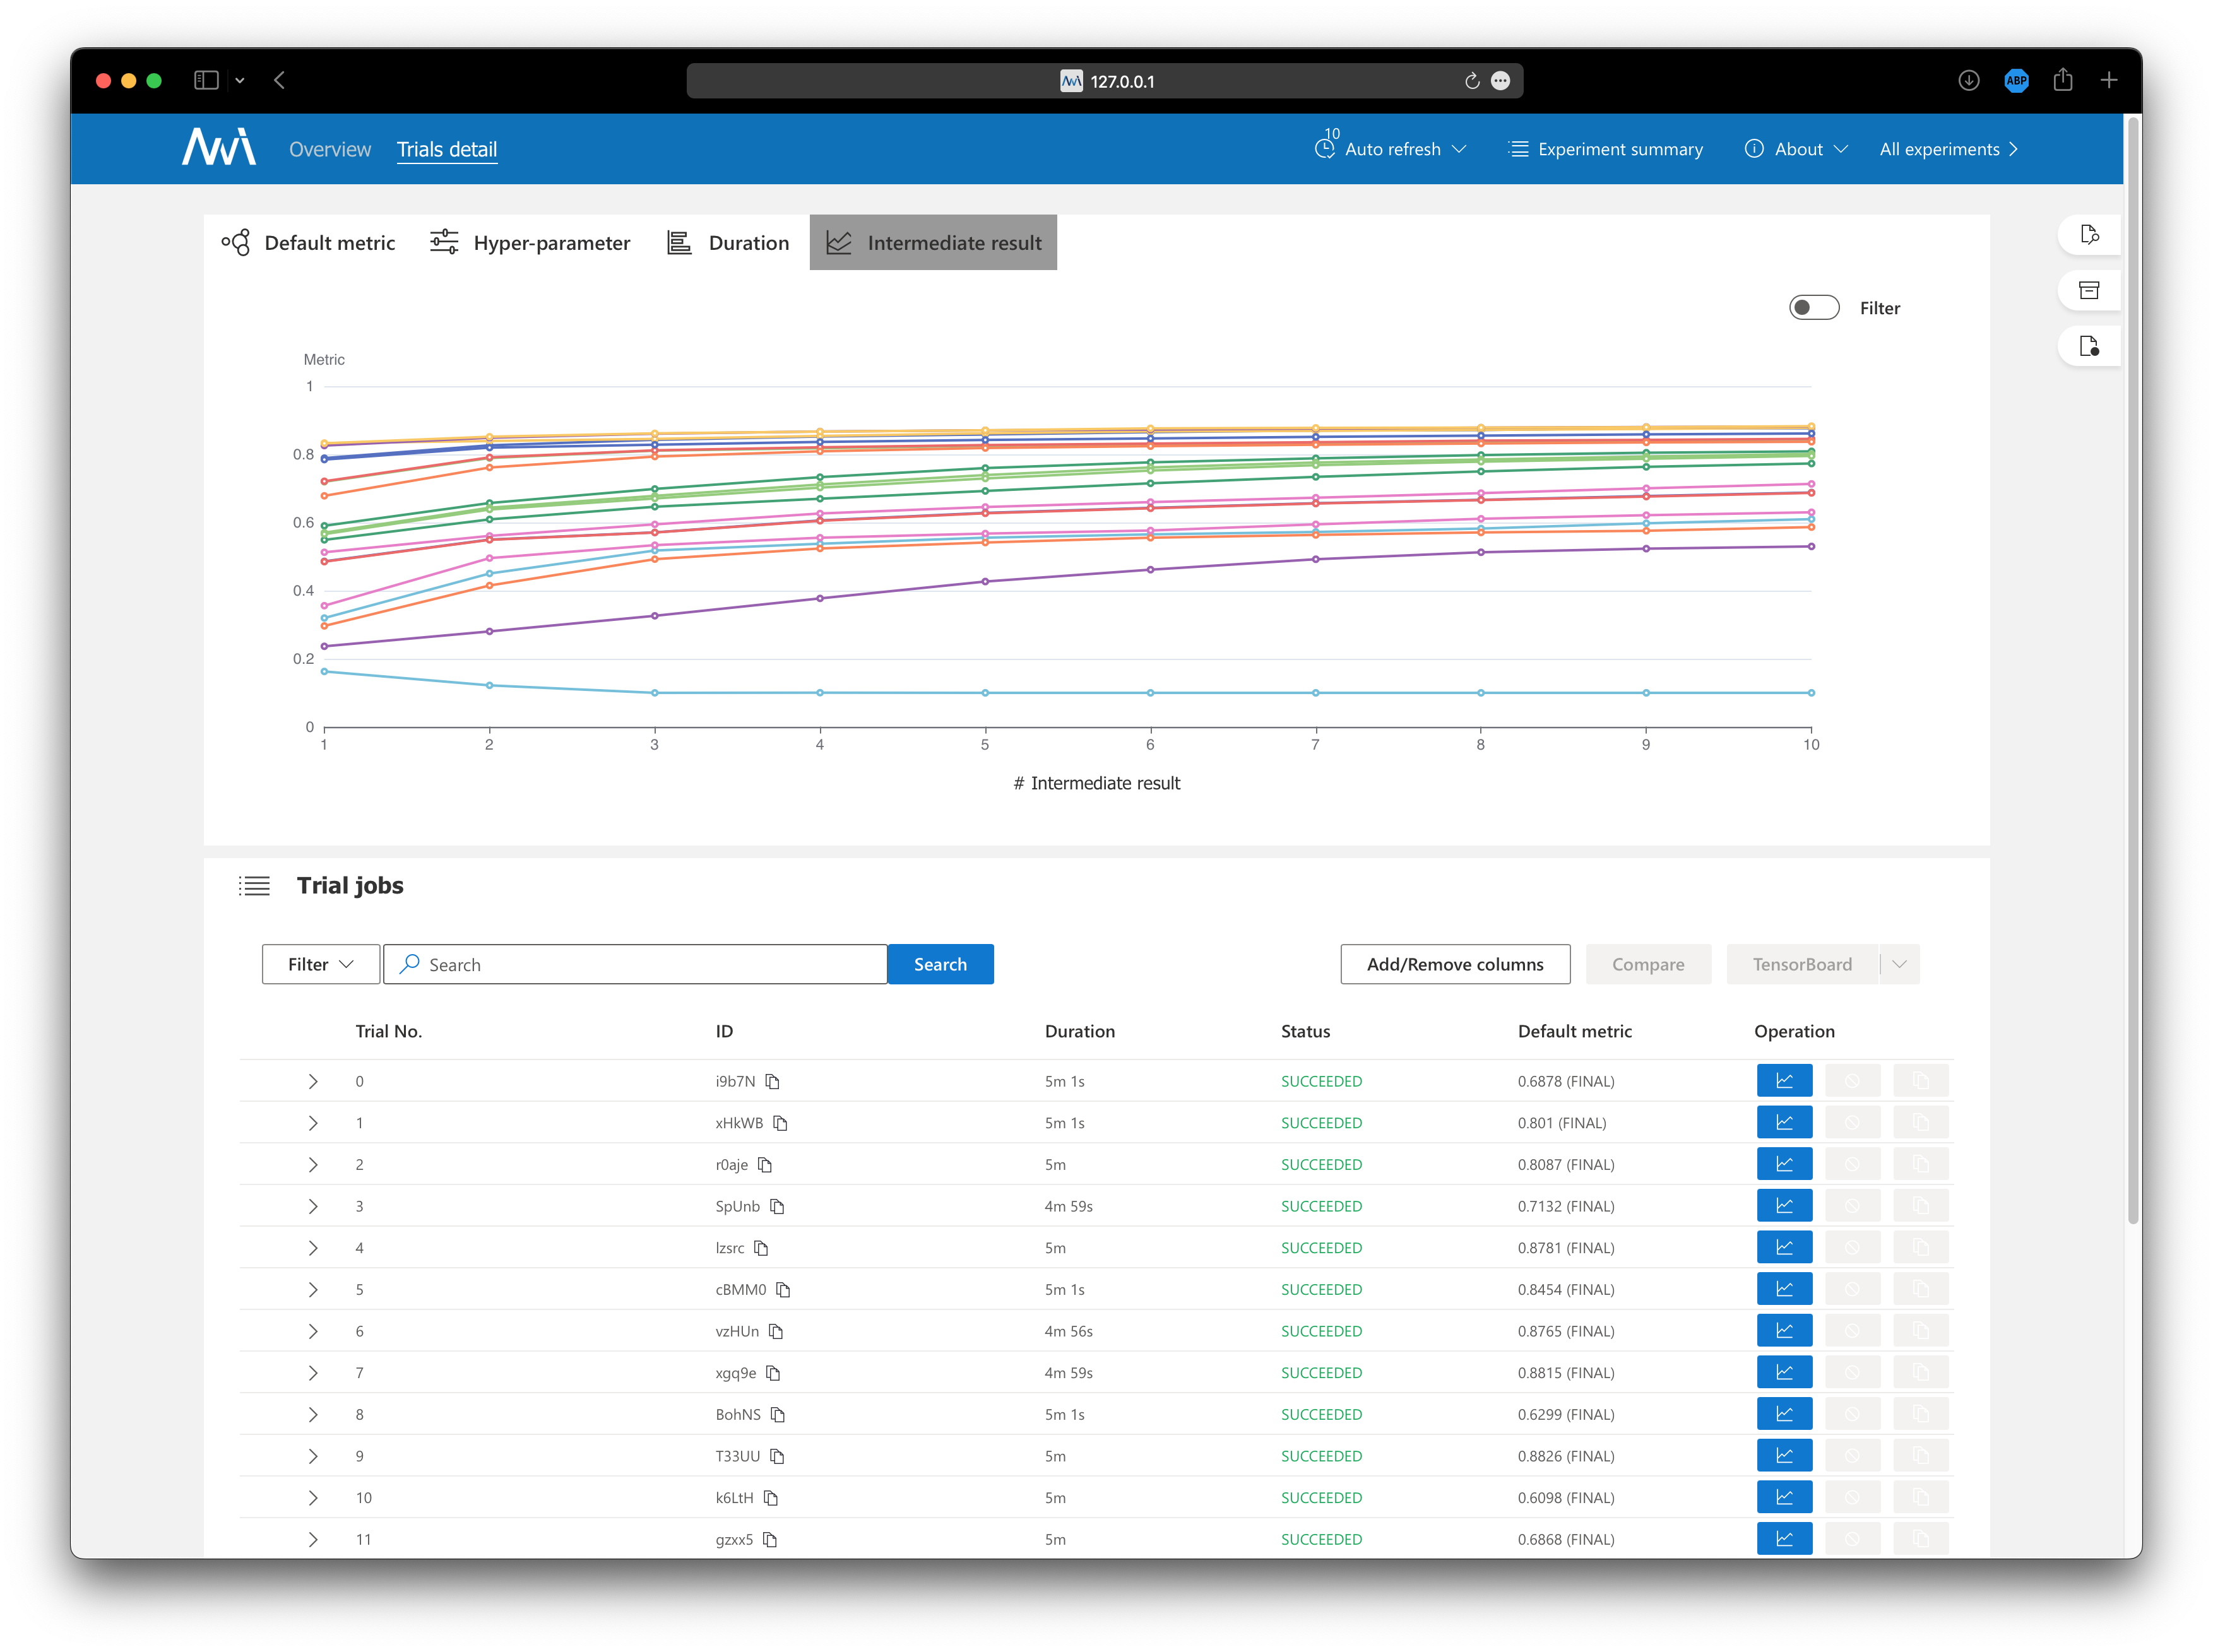
\includegraphics[width=3.5in]{../proj3/figures/mlp_tpe_intermediate.png}}
    \caption{MLP with TPE Tuner on Learning Rate and Momentum}
    \label{fig:mlp-tpe}
\end{figure}

Figure \ref{fig:mlp-evolution} shows the result of the MLP with Evolution. We observe that Trial 13 has the most optimal parameters with a validation accuracy of 87.98\%. The optimal parameters for this trial are a learning rate of $0.0269$ and a momentum of $0.5765$. We also observe that the duration for all trials is about 5 minutes.

\begin{figure}
    \centerline{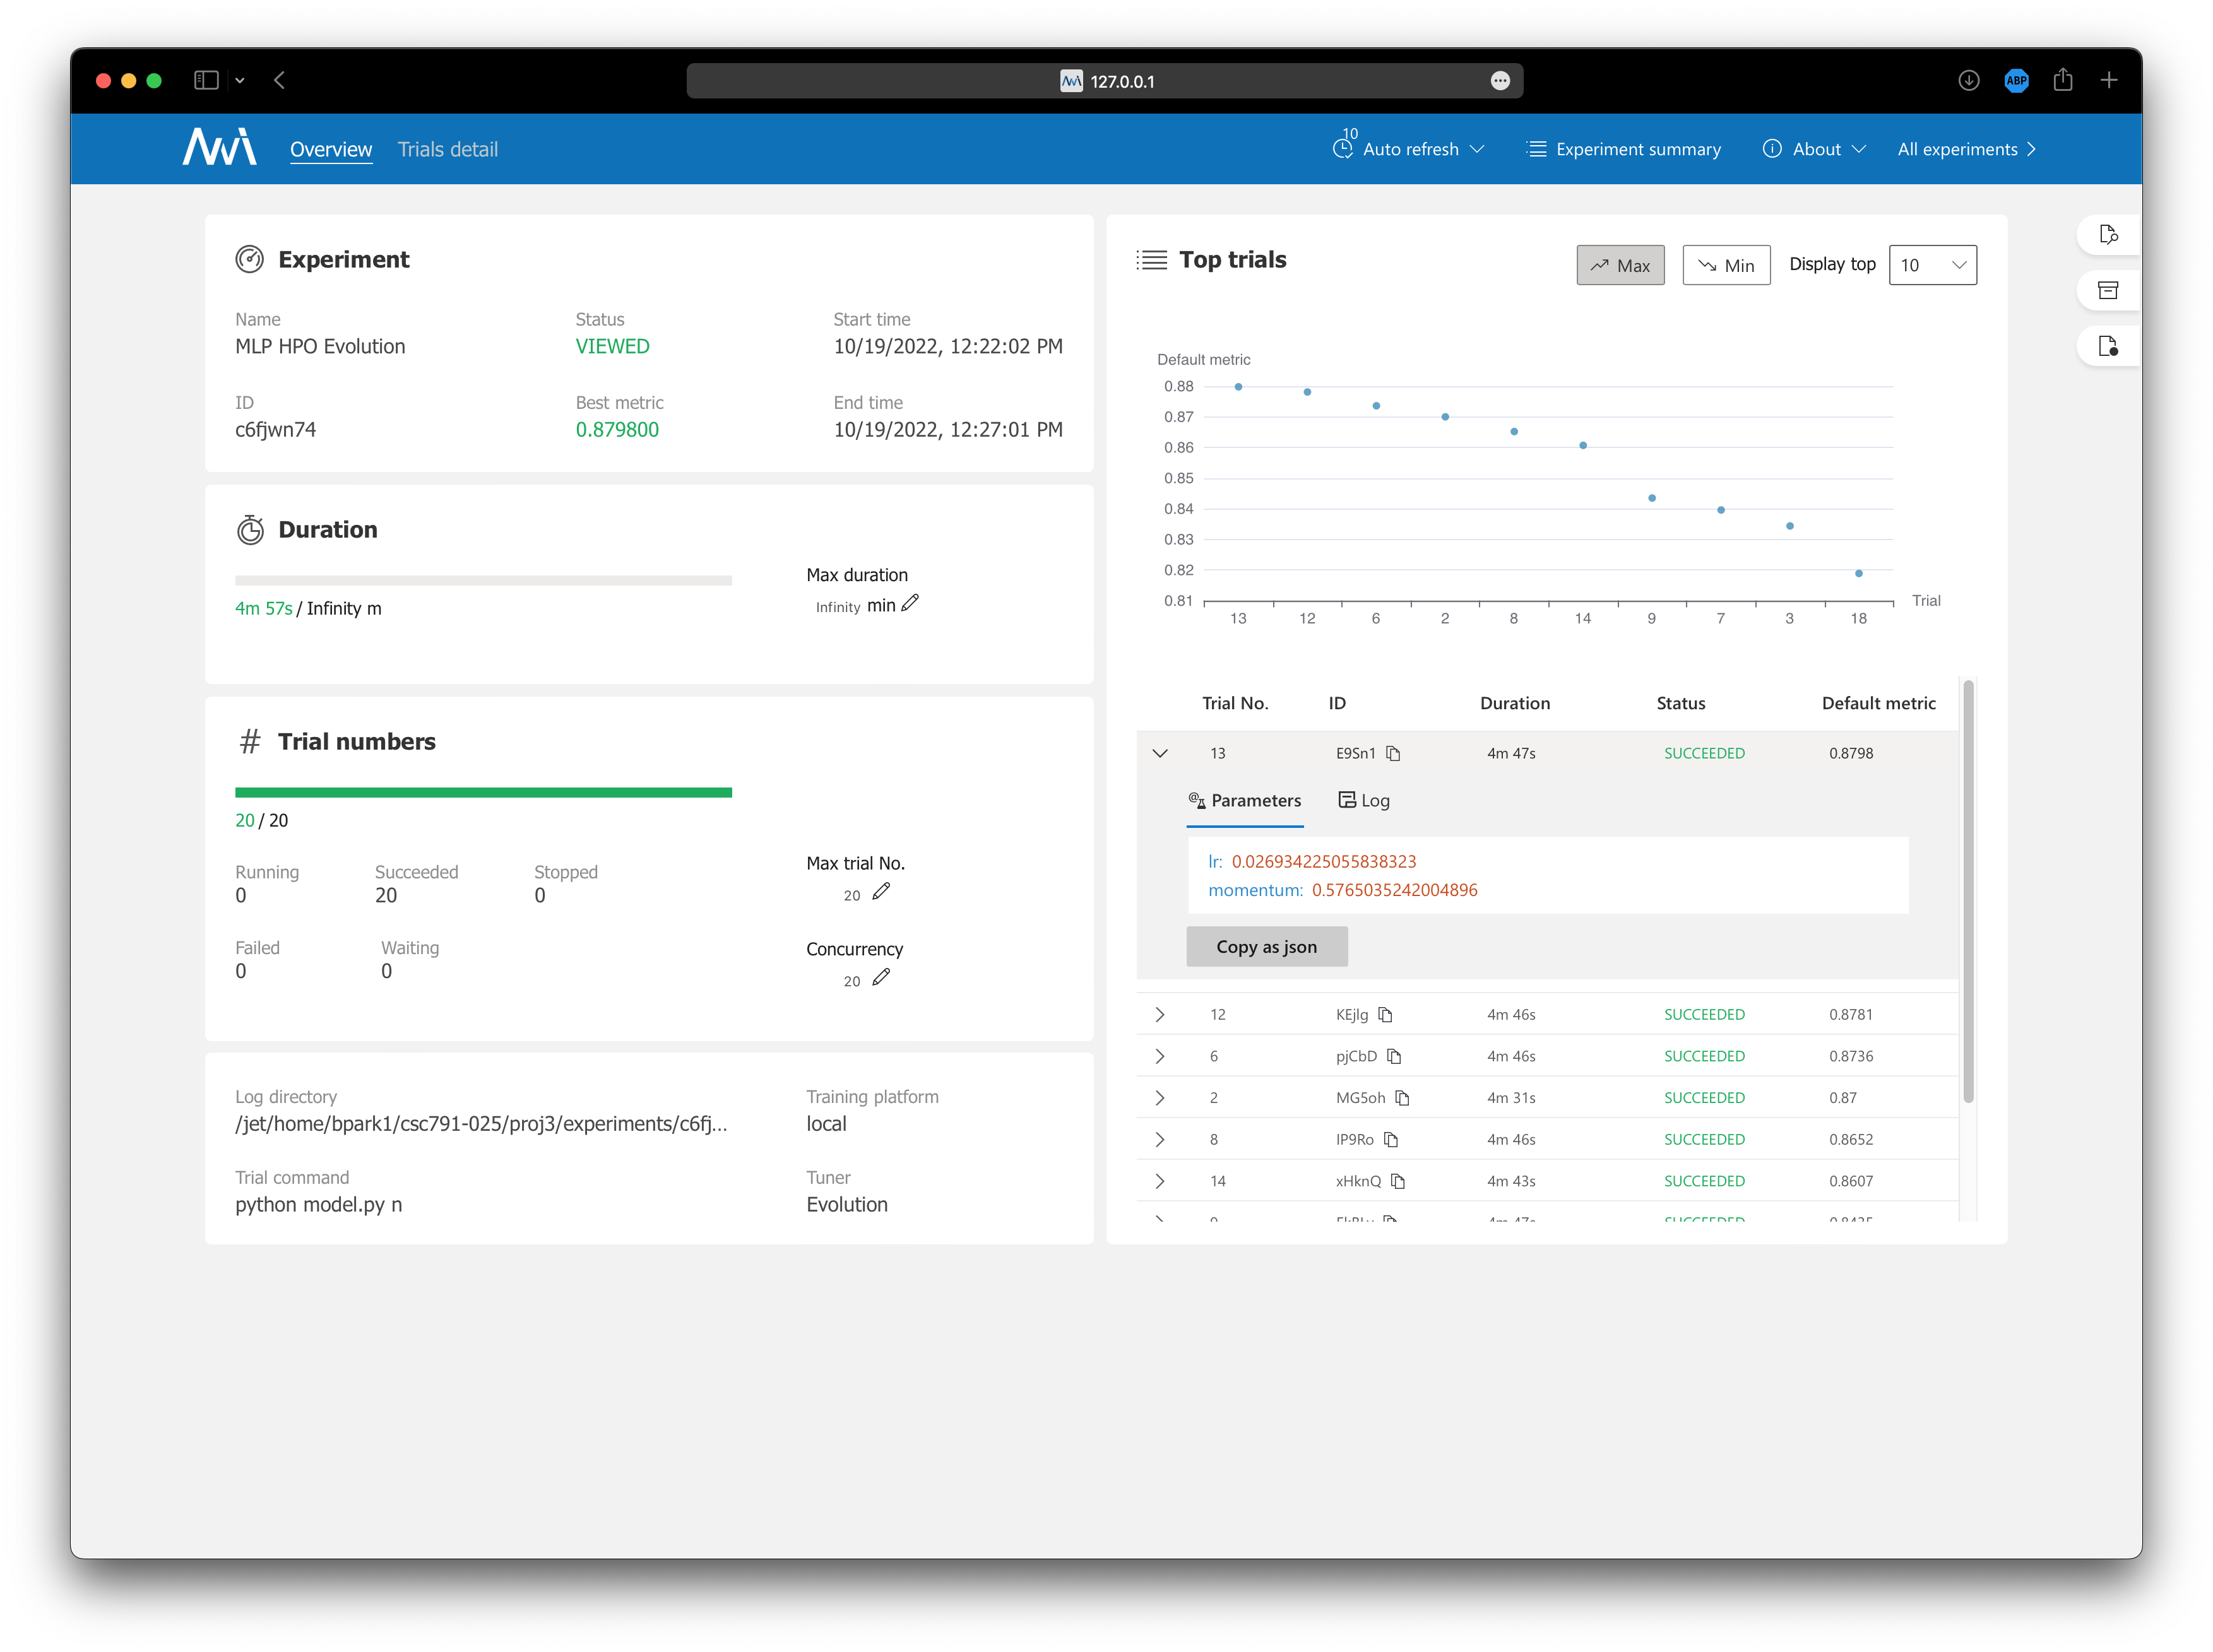
\includegraphics[width=3.5in]{../proj3/figures/mlp_evolution_overview.png}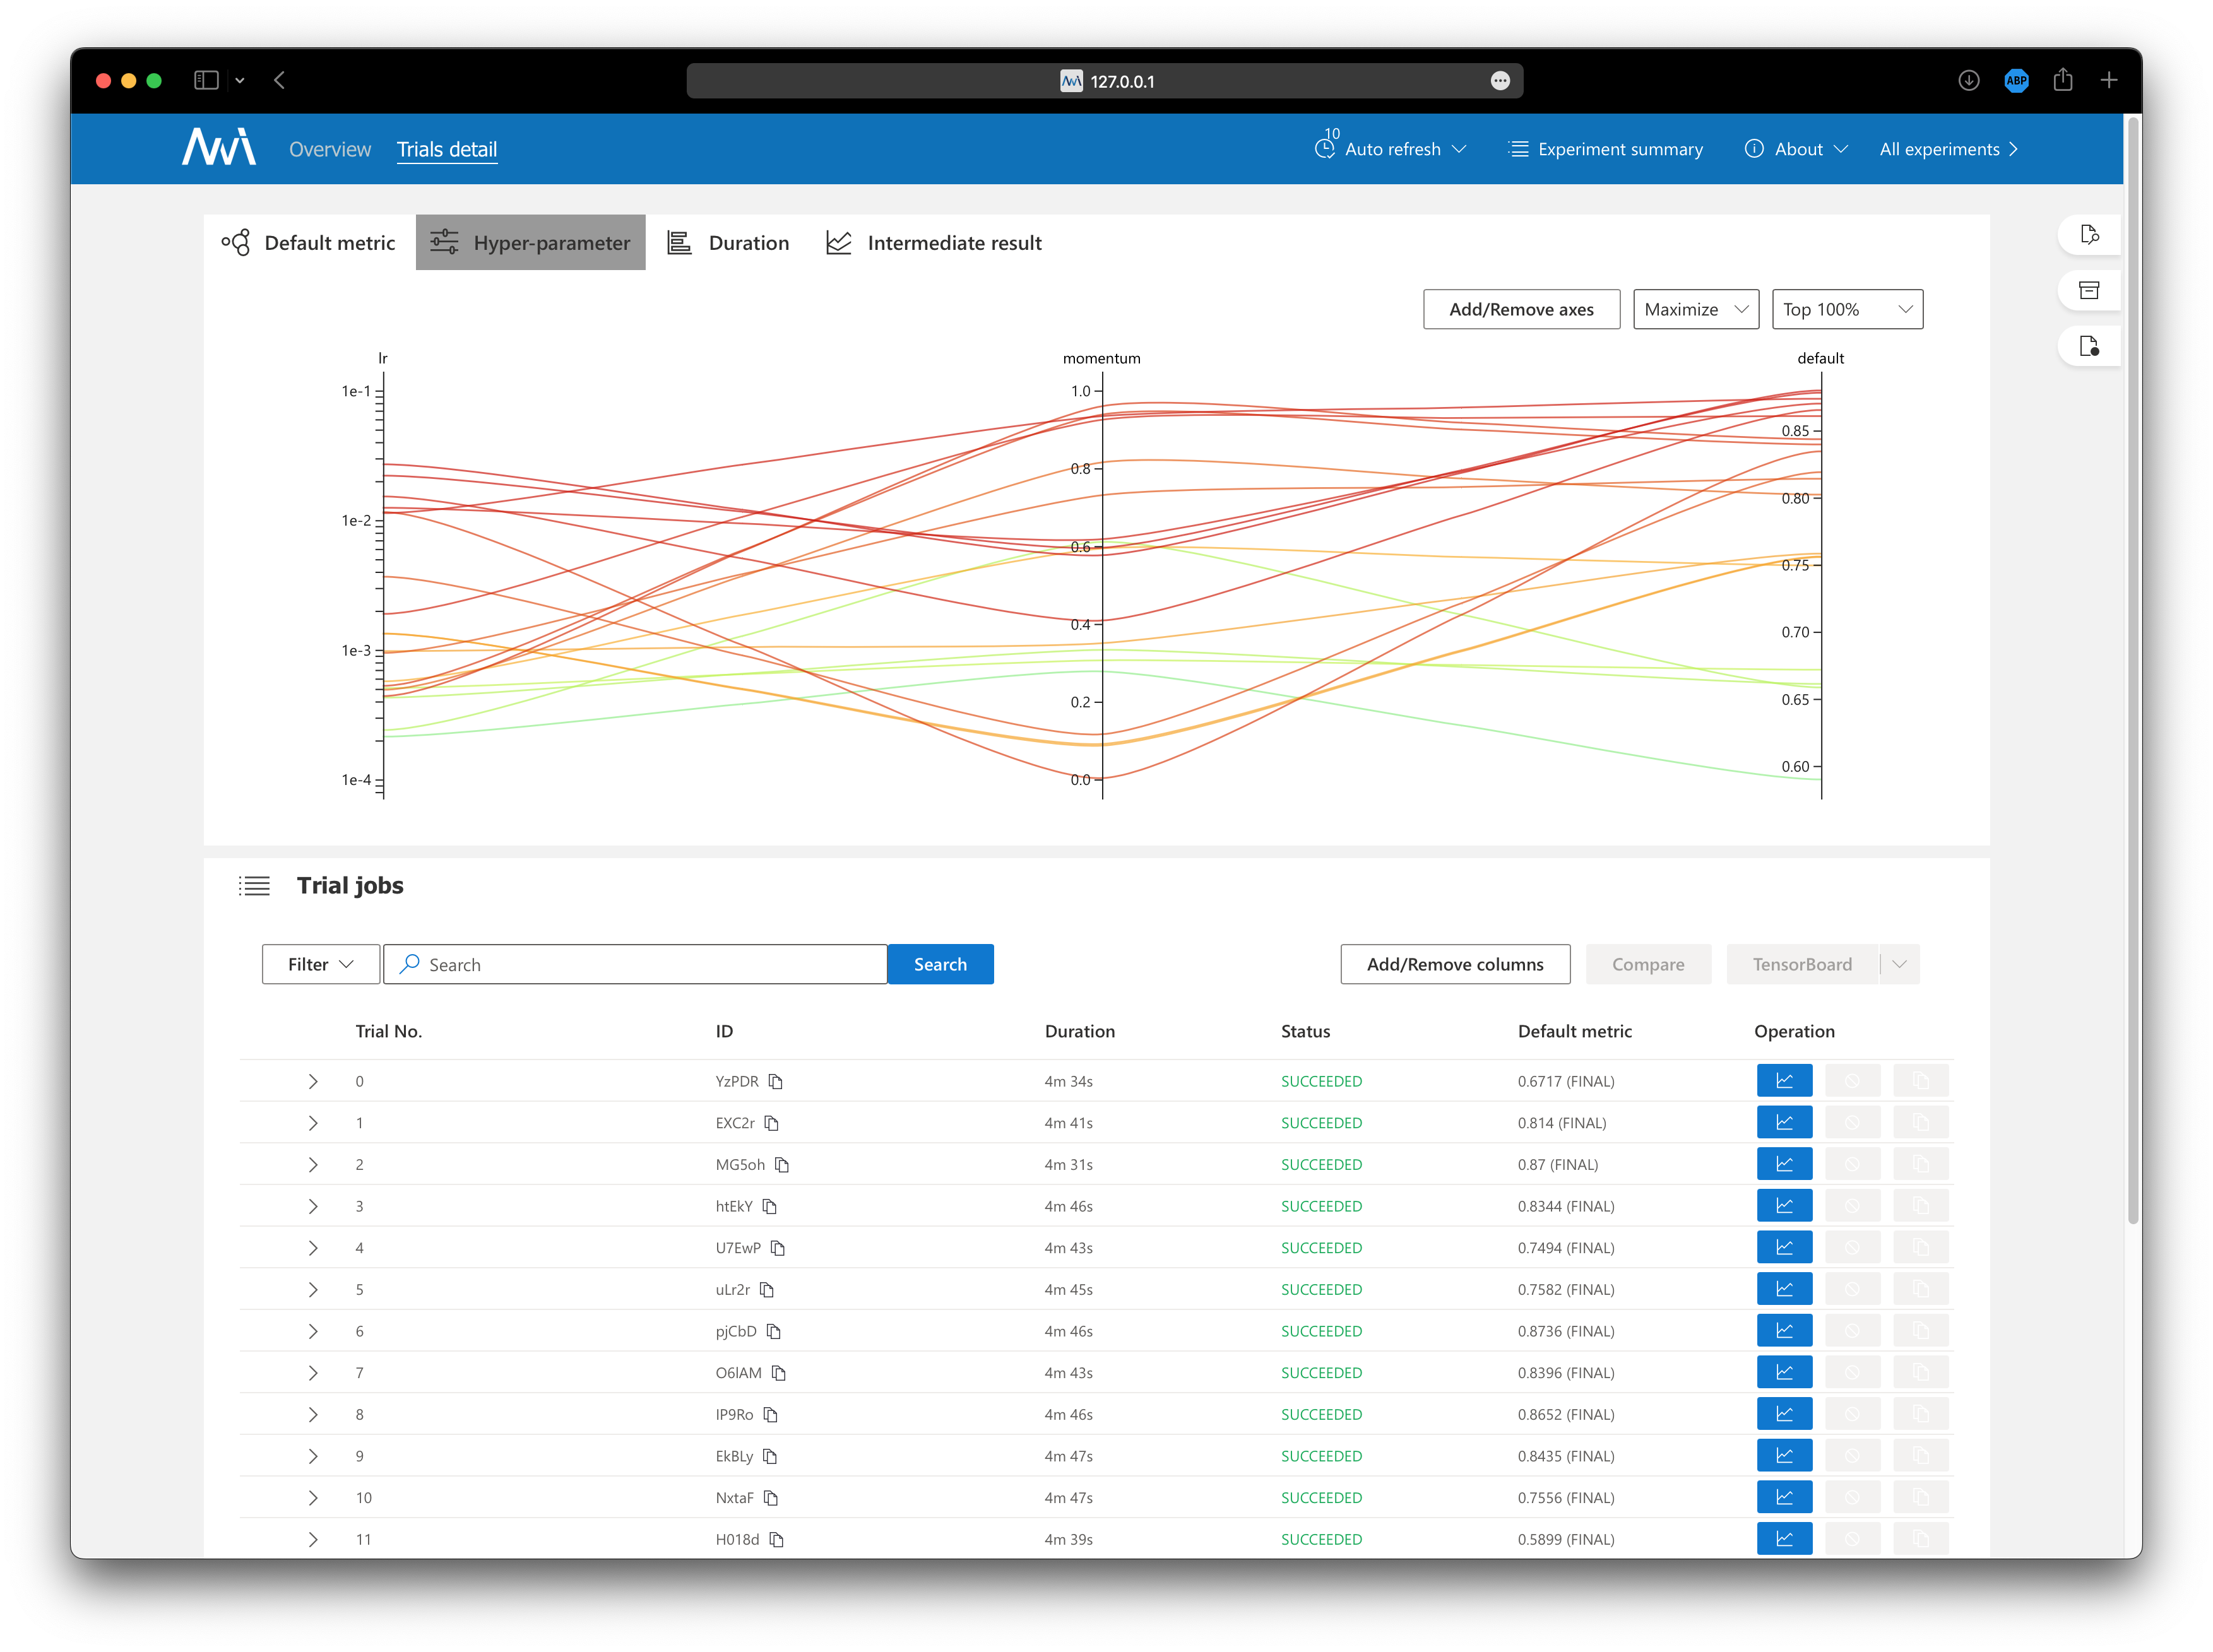
\includegraphics[width=3.5in]{../proj3/figures/mlp_evolution_hyperparameter.png}}
    \centerline{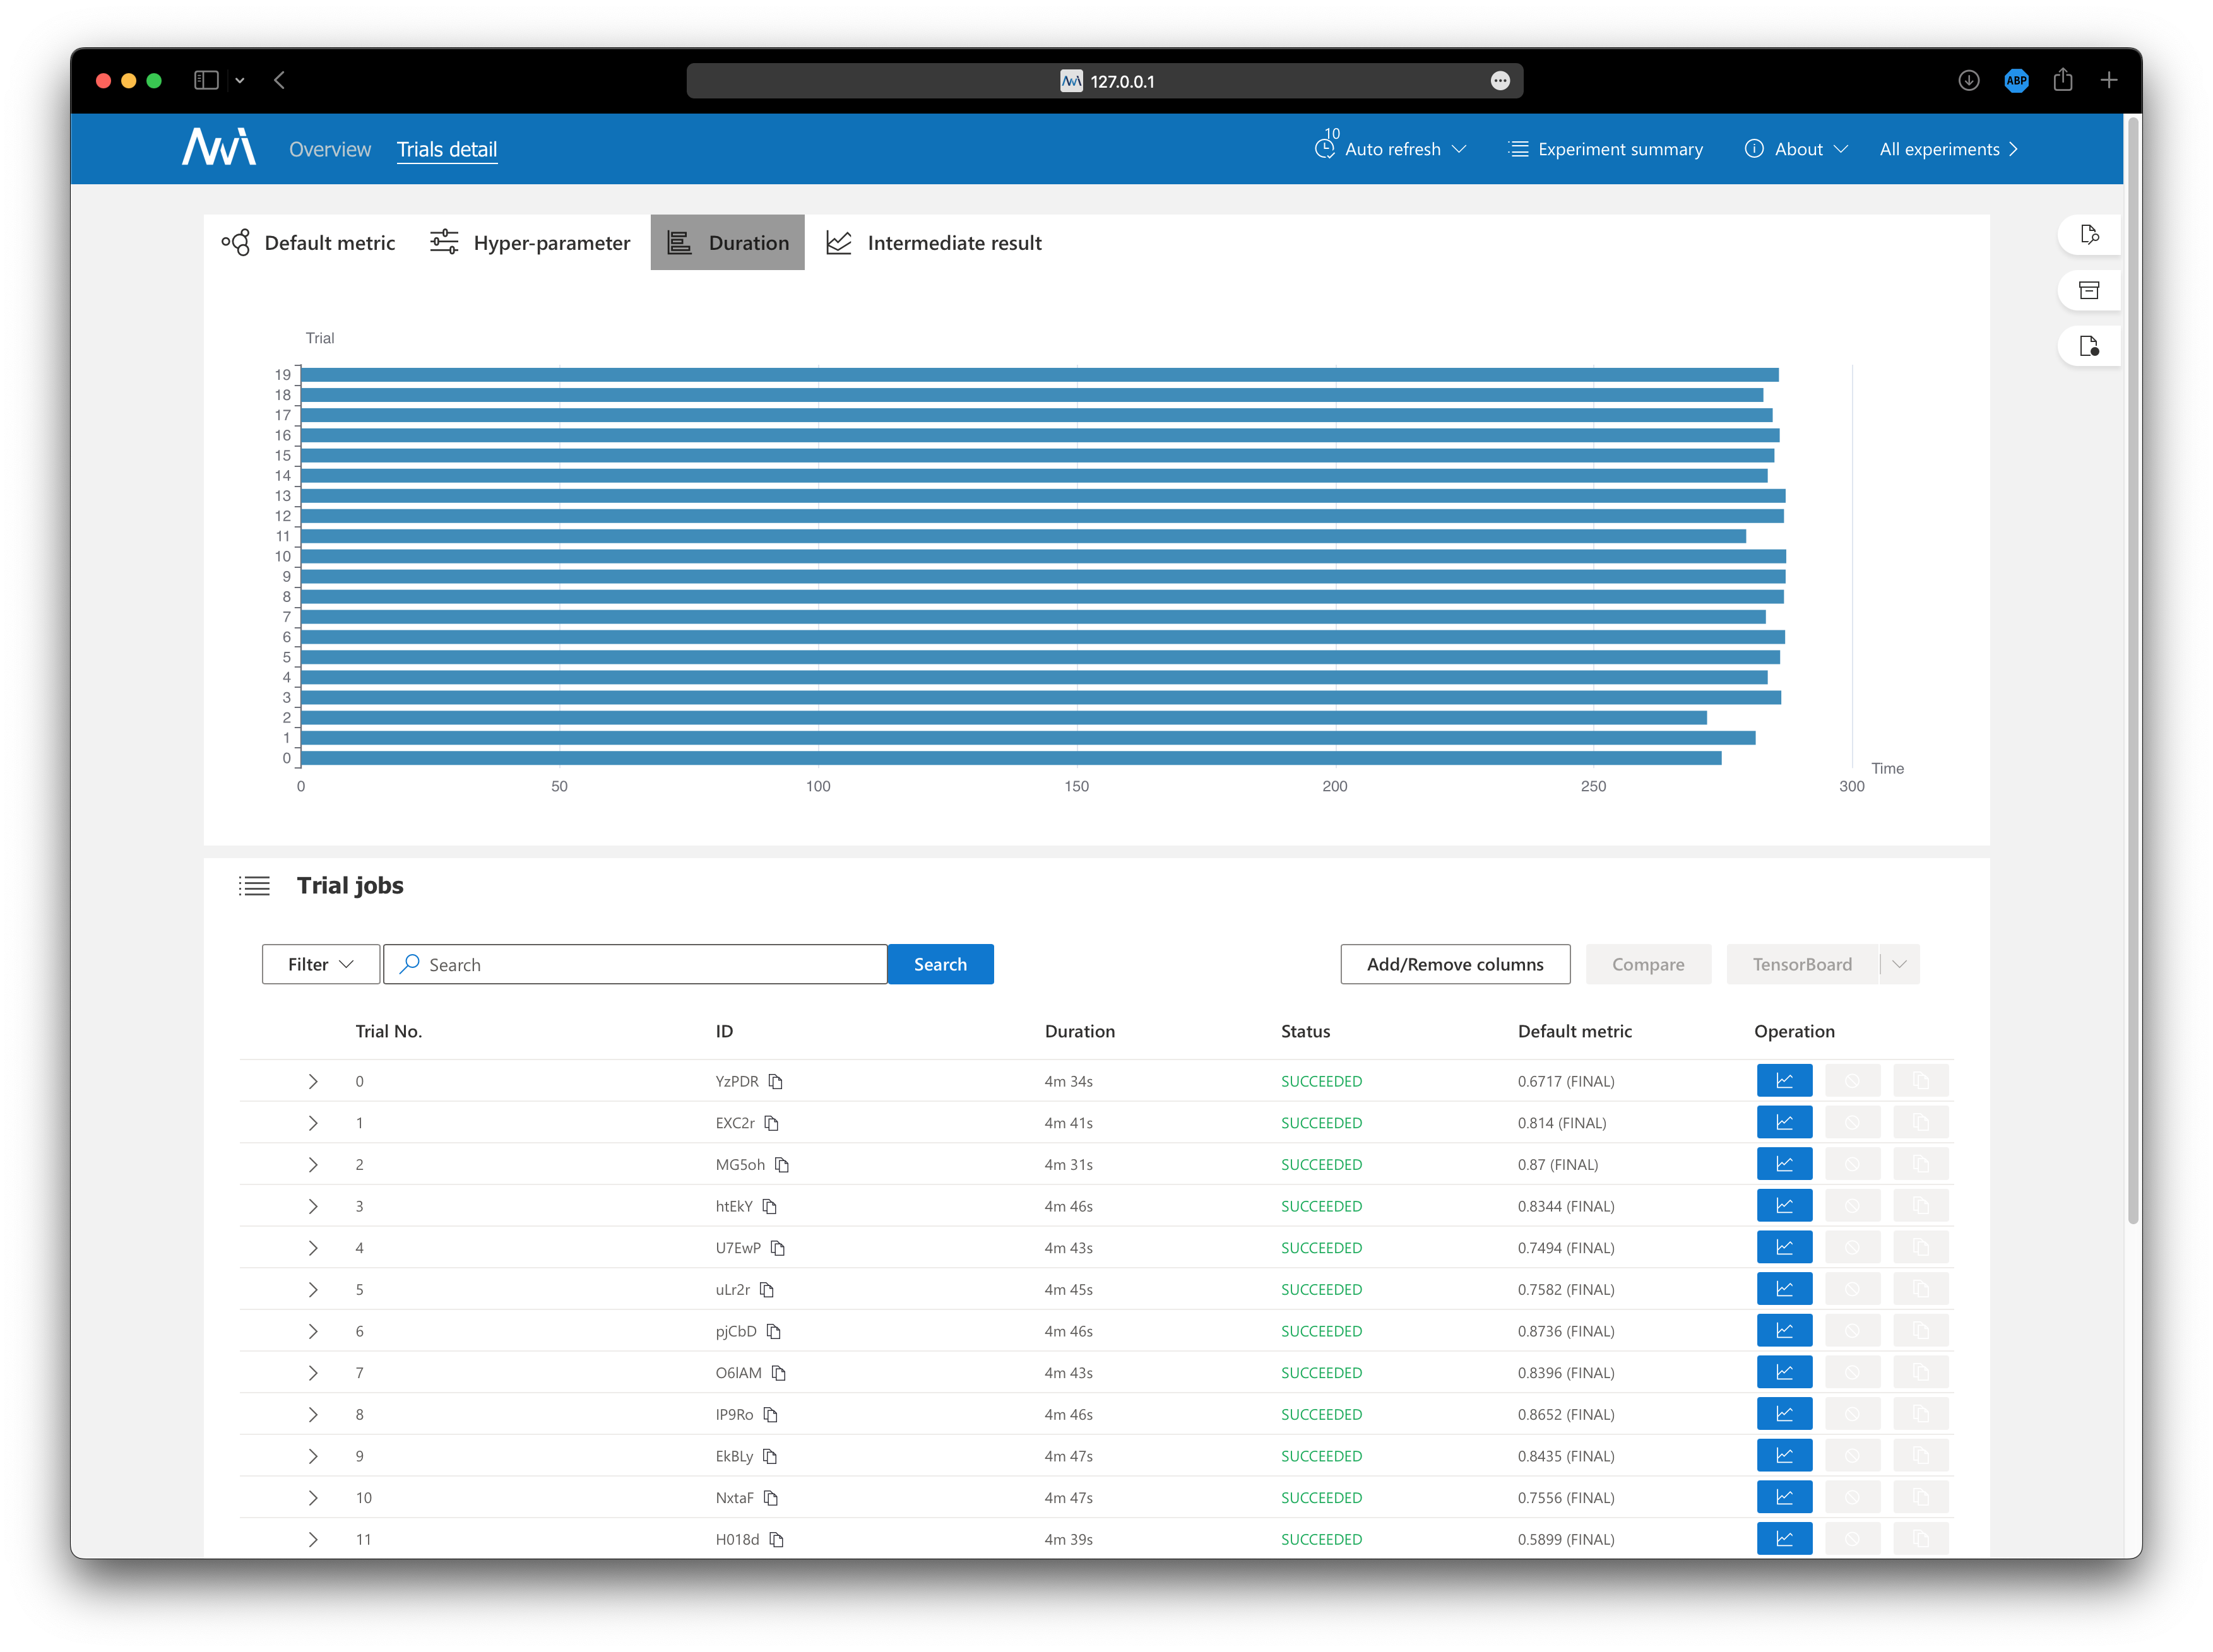
\includegraphics[width=3.5in]{../proj3/figures/mlp_evolution_latency.png}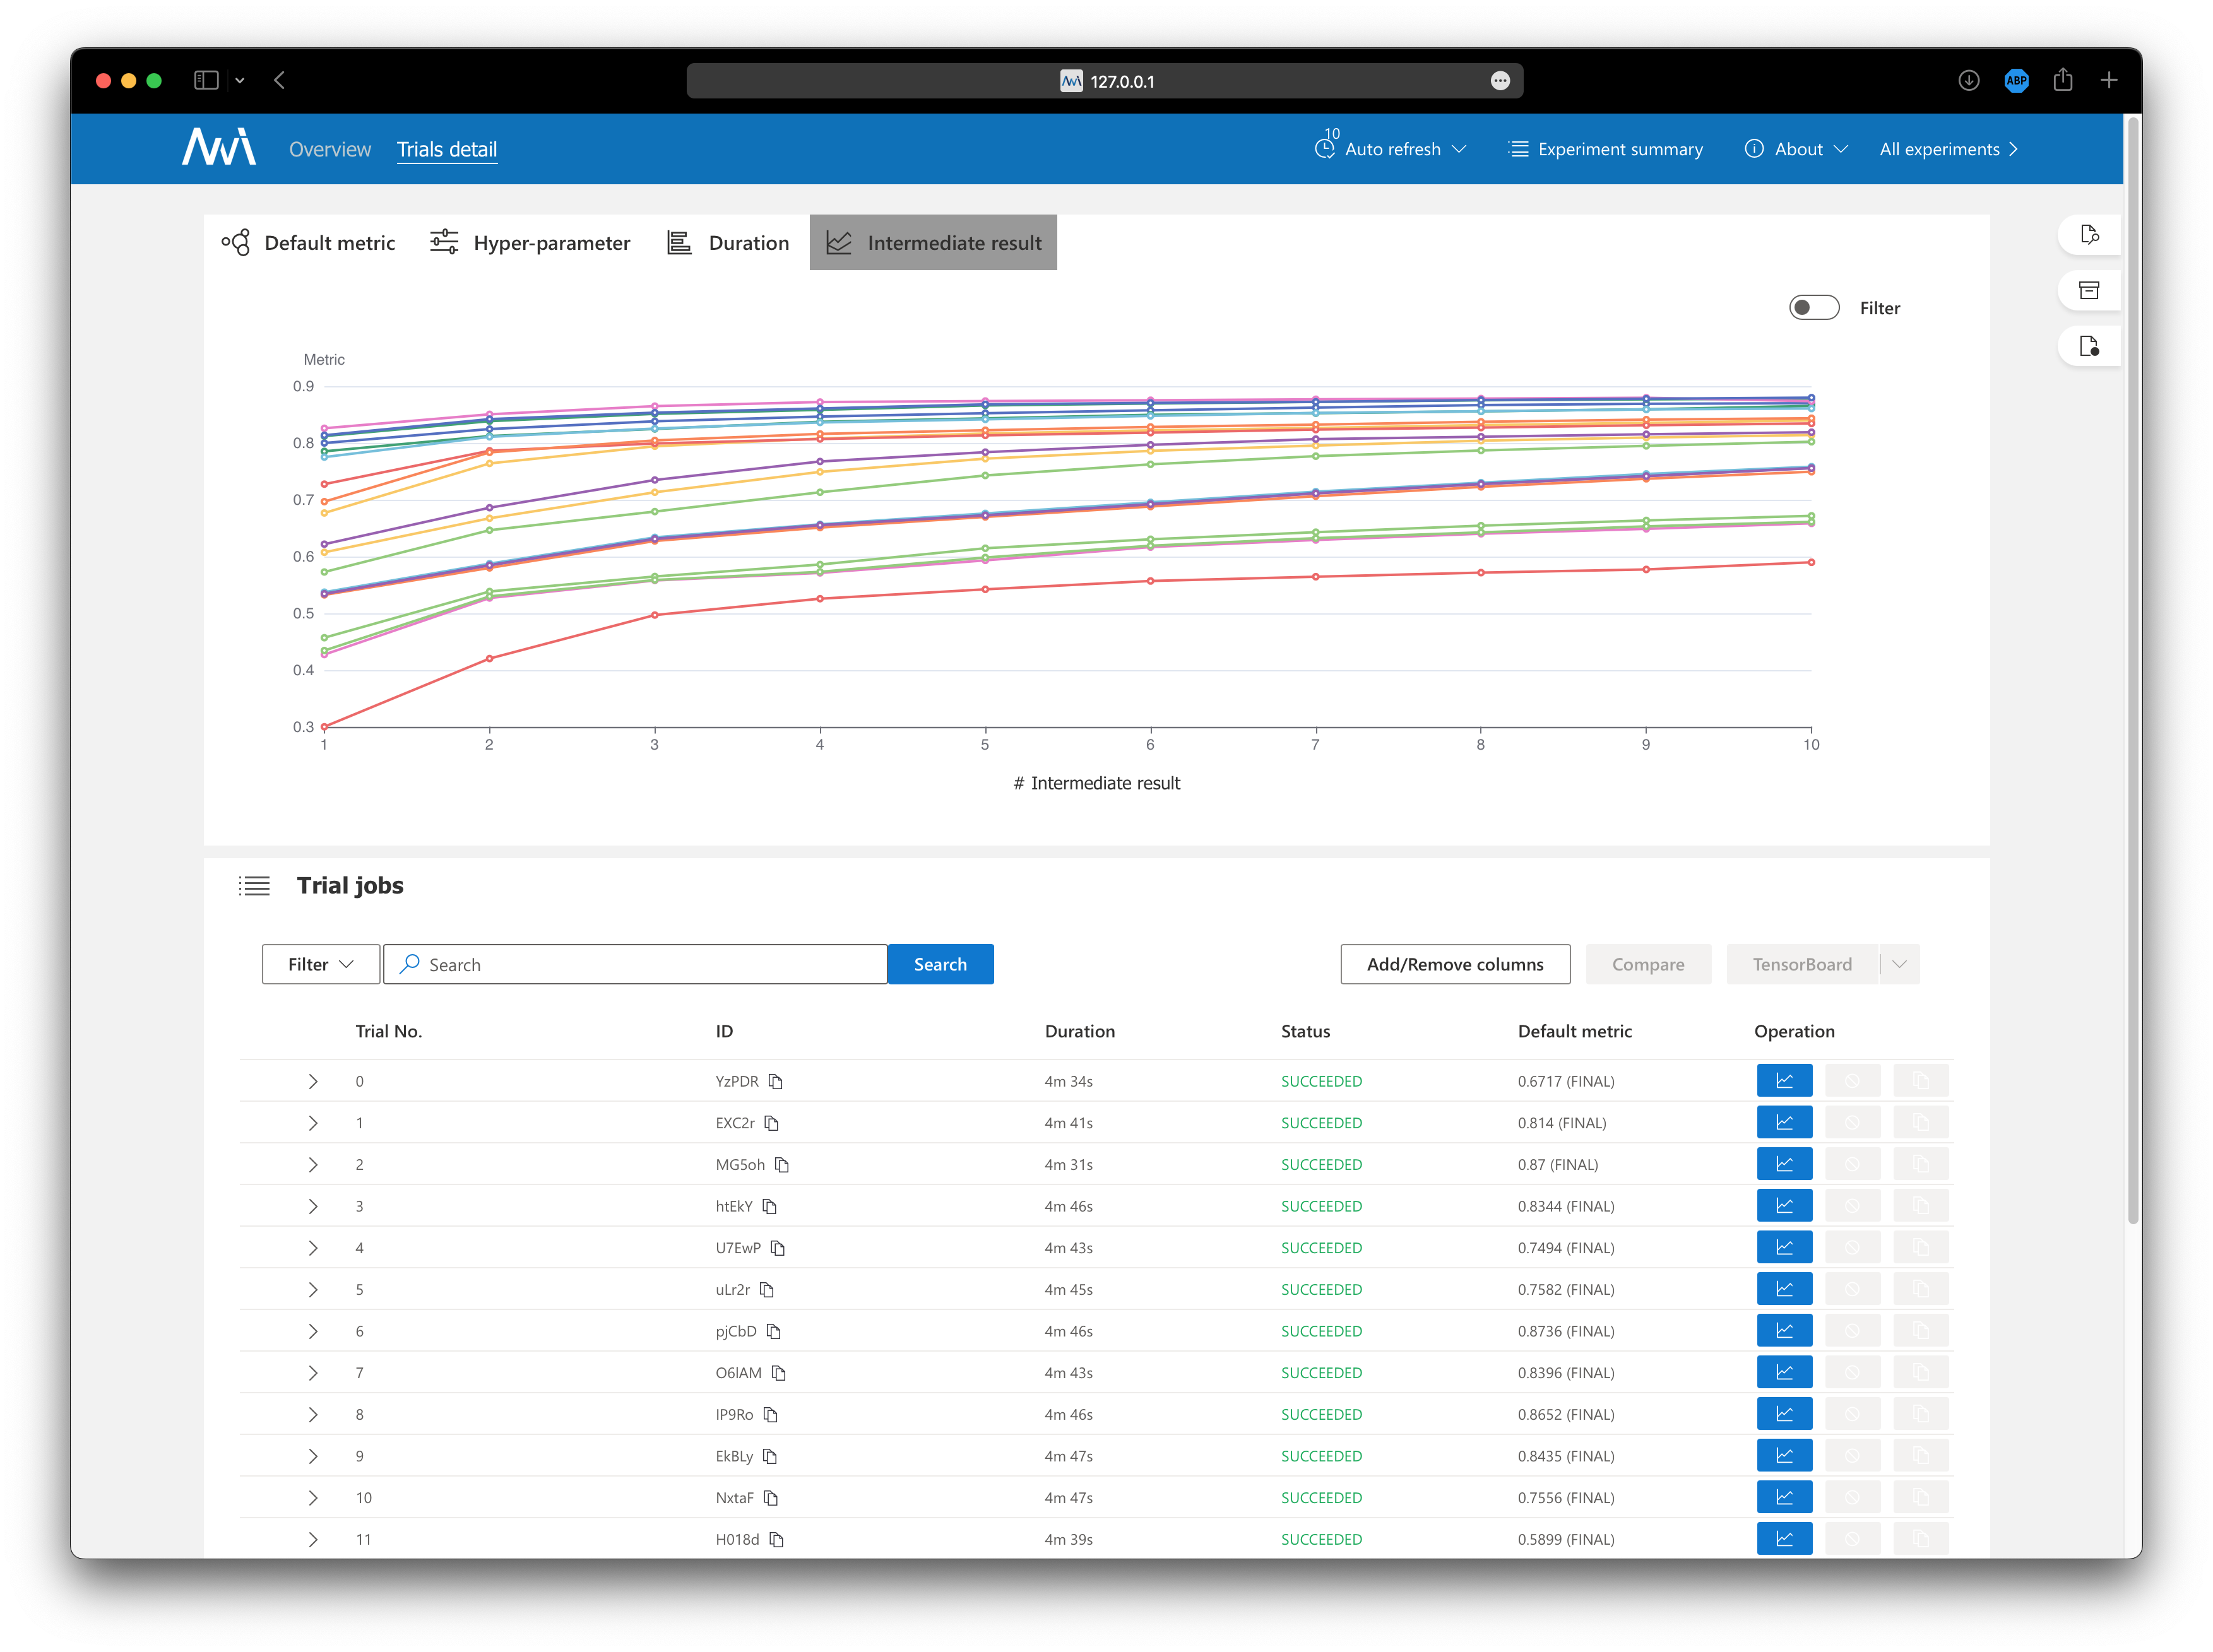
\includegraphics[width=3.5in]{../proj3/figures/mlp_evolution_intermediate.png}}
    \caption{MLP with Evolution Tuner on Learning Rate and Momentum}
    \label{fig:mlp-evolution}
\end{figure}

Figure \ref{fig:mlp-hyperband} shows the result of the MLP with Evolution. We observe that Trial 2 has the most optimal parameters with a validation accuracy of 88.33\%. The optimal parameters for this trial are a learning rate of $0.0855$ and a momentum of $0.6975$. We also observe that the duration for all trials is also about 5 minutes.

\begin{figure}
    \centerline{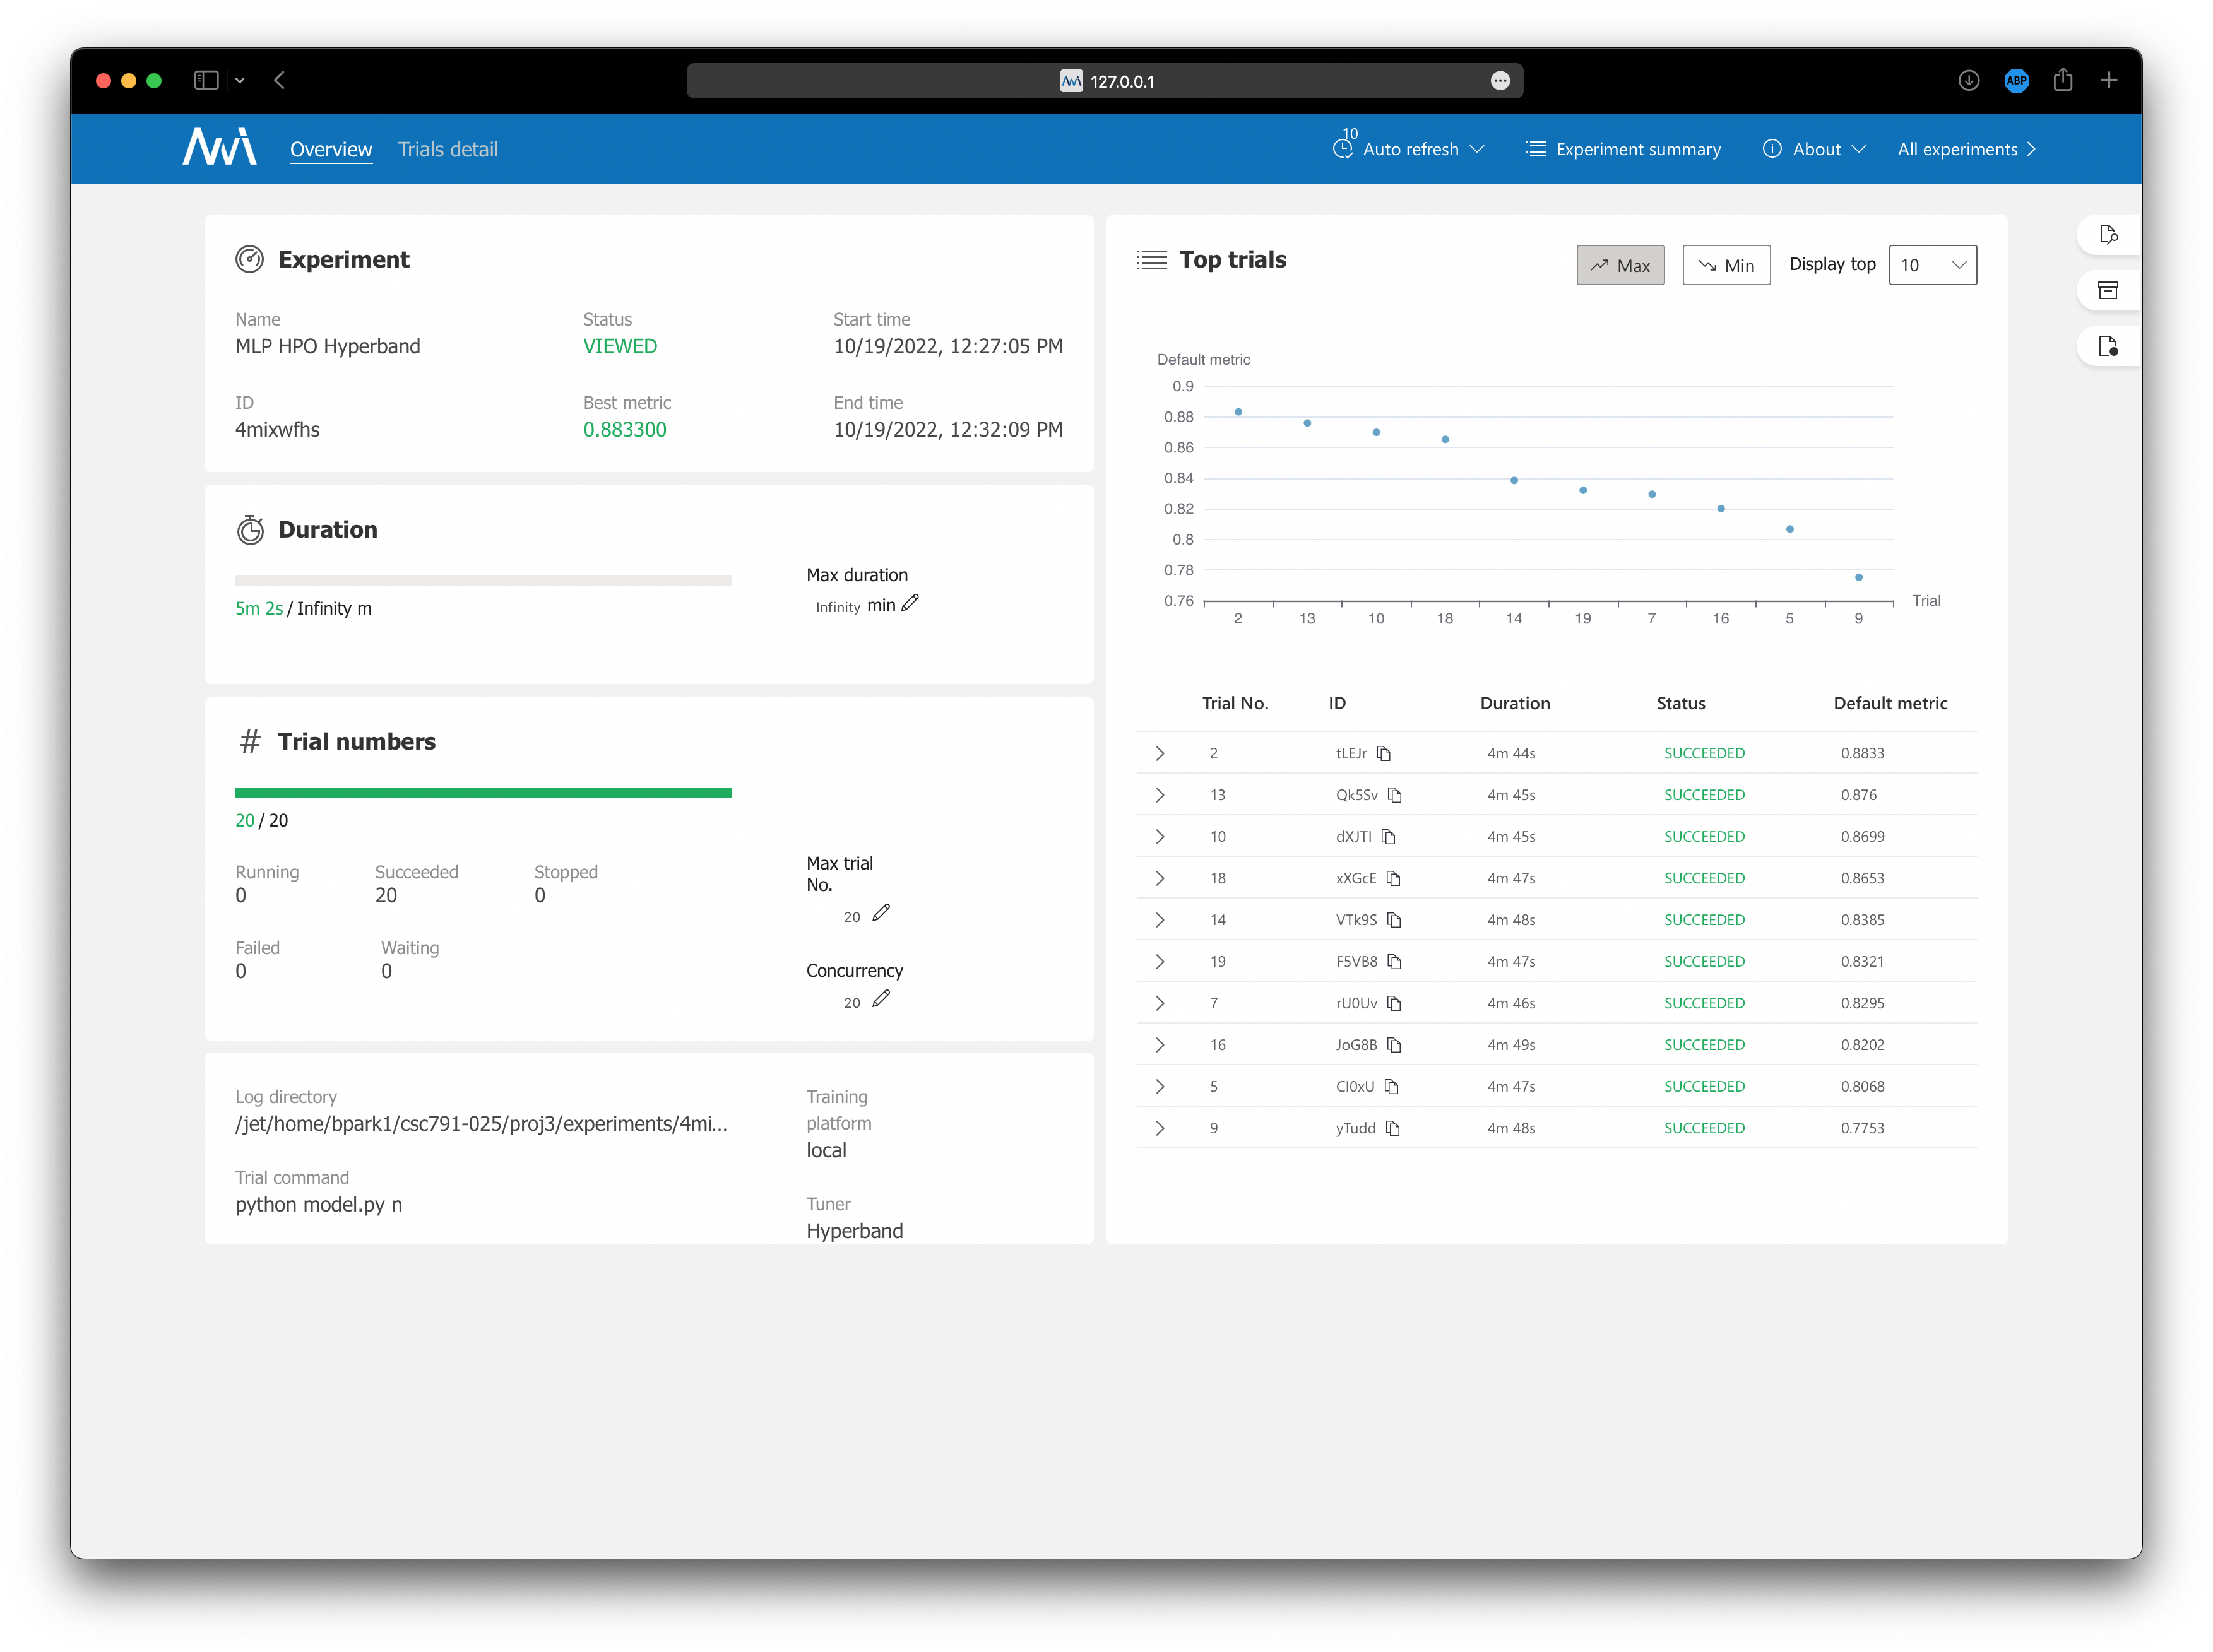
\includegraphics[width=3.5in]{../proj3/figures/mlp_hyperband_overview.png}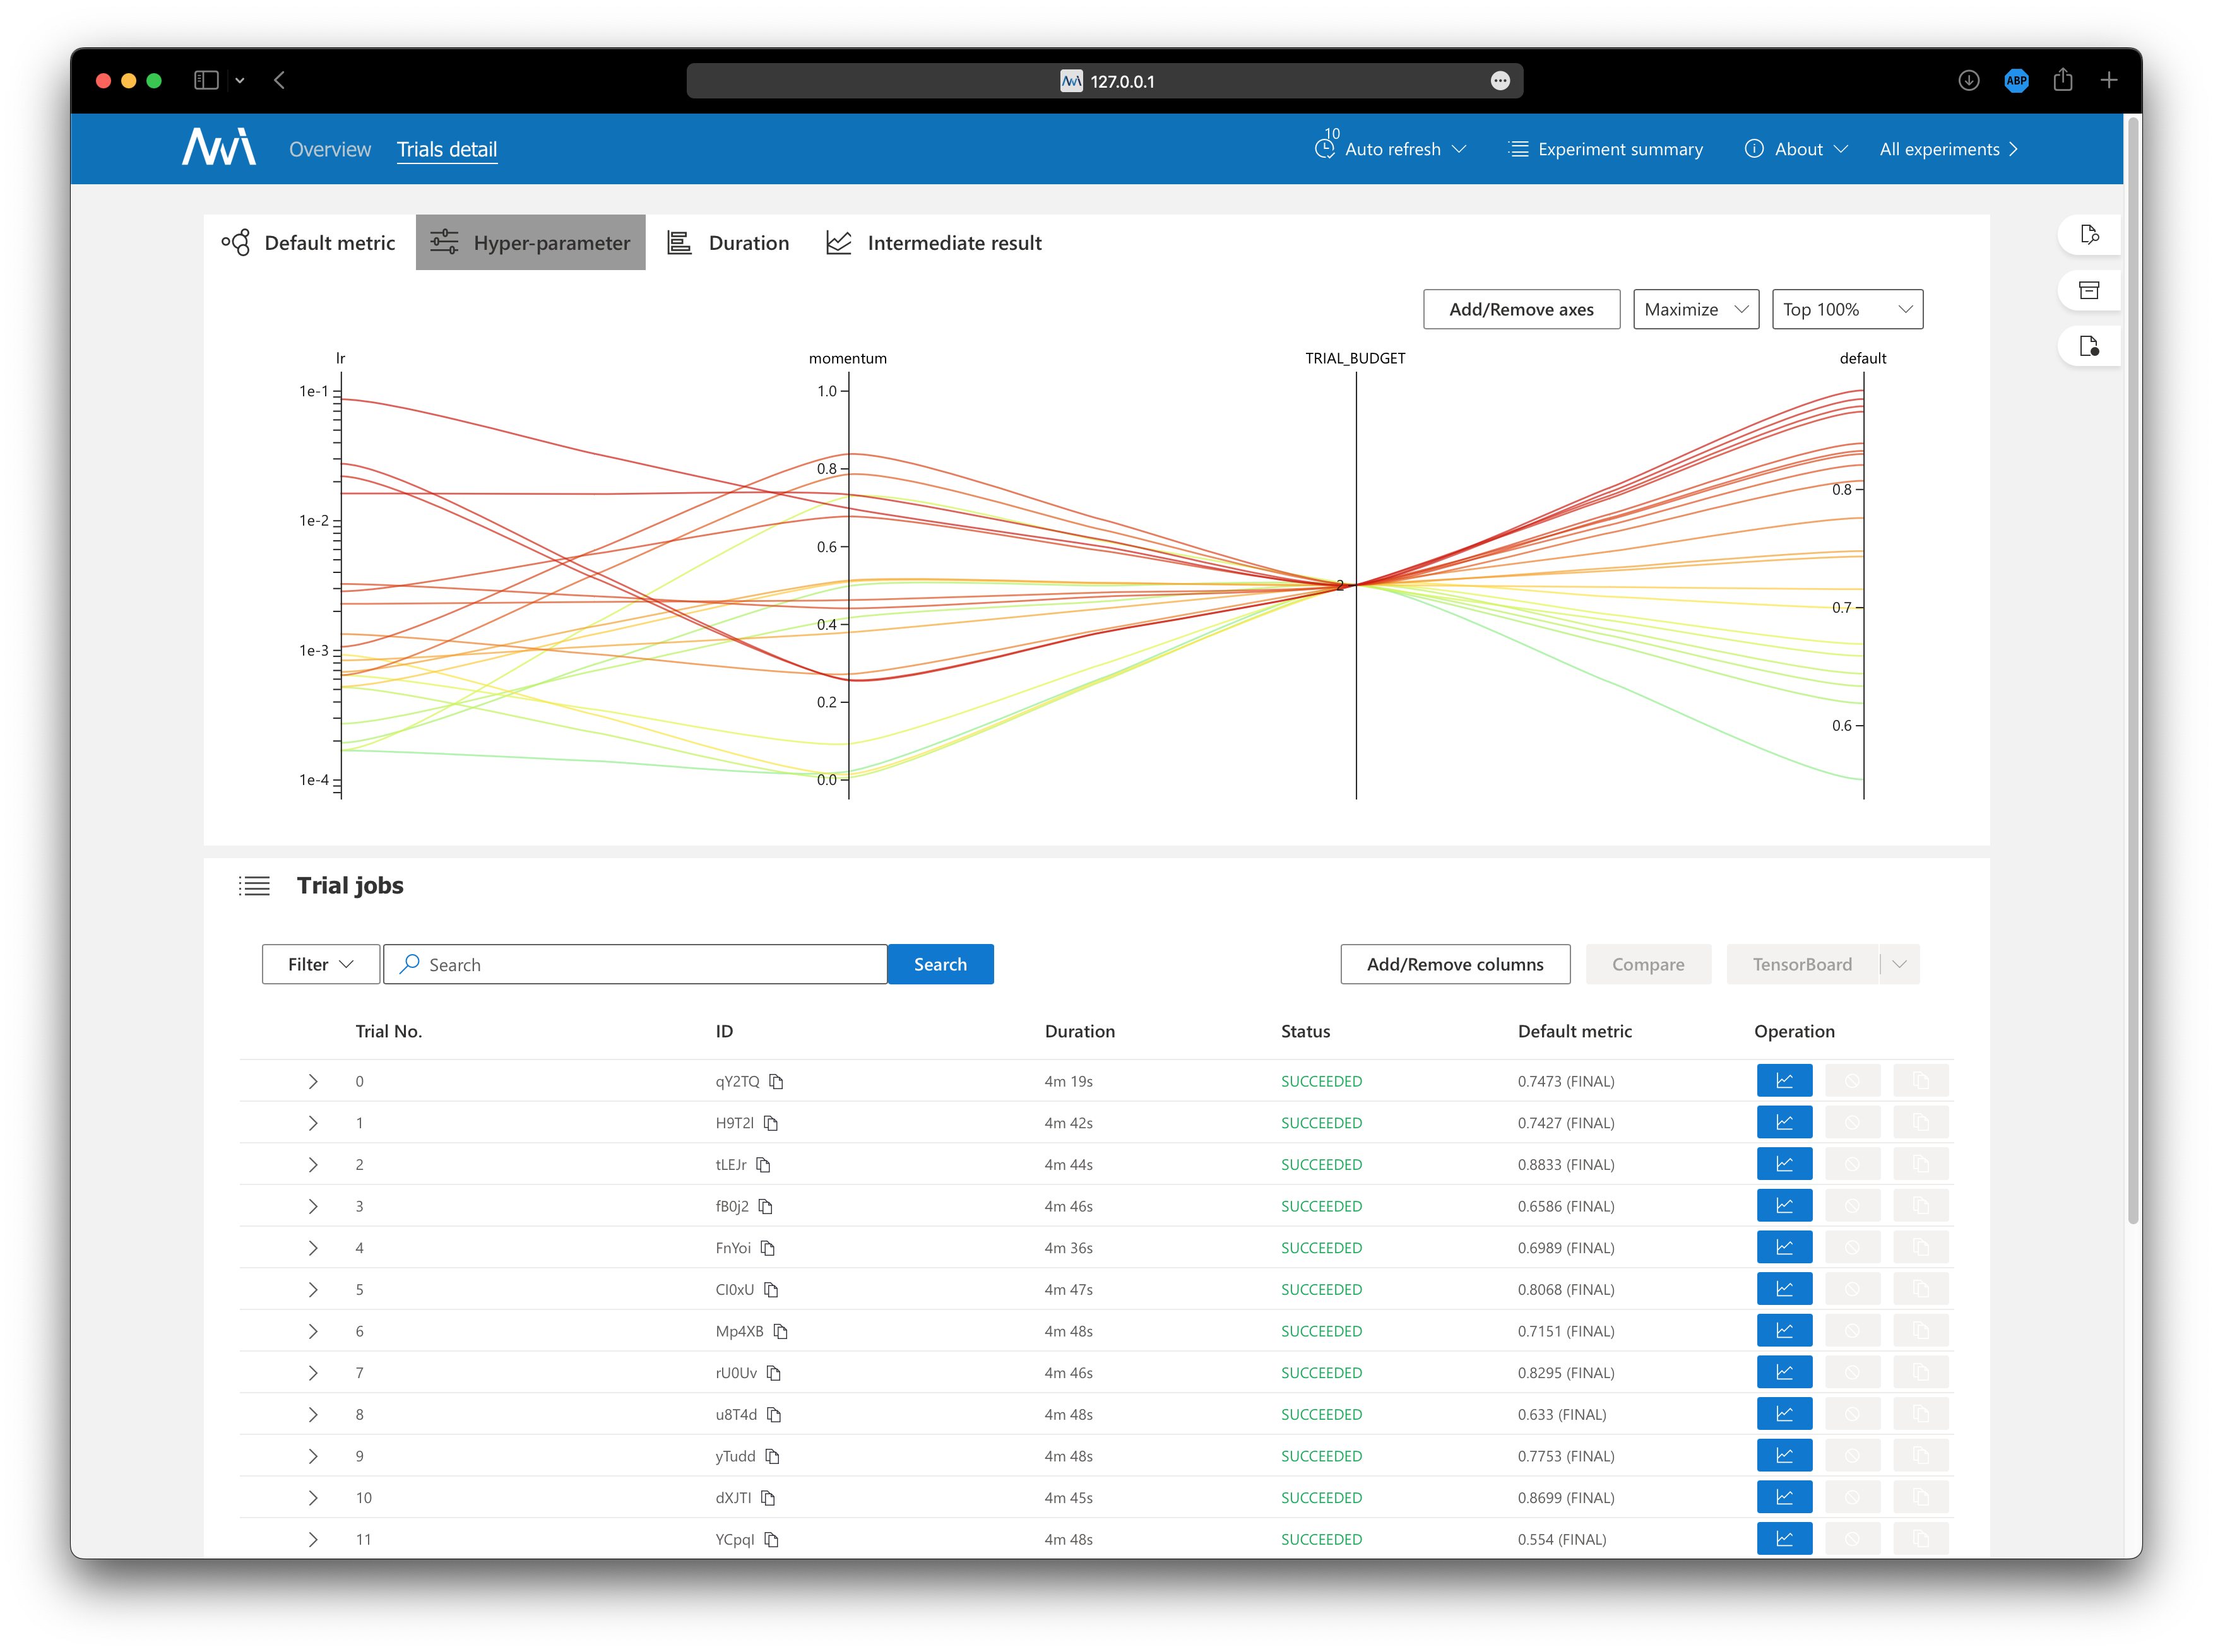
\includegraphics[width=3.5in]{../proj3/figures/mlp_hyperband_hyperparameter.png}}
    \centerline{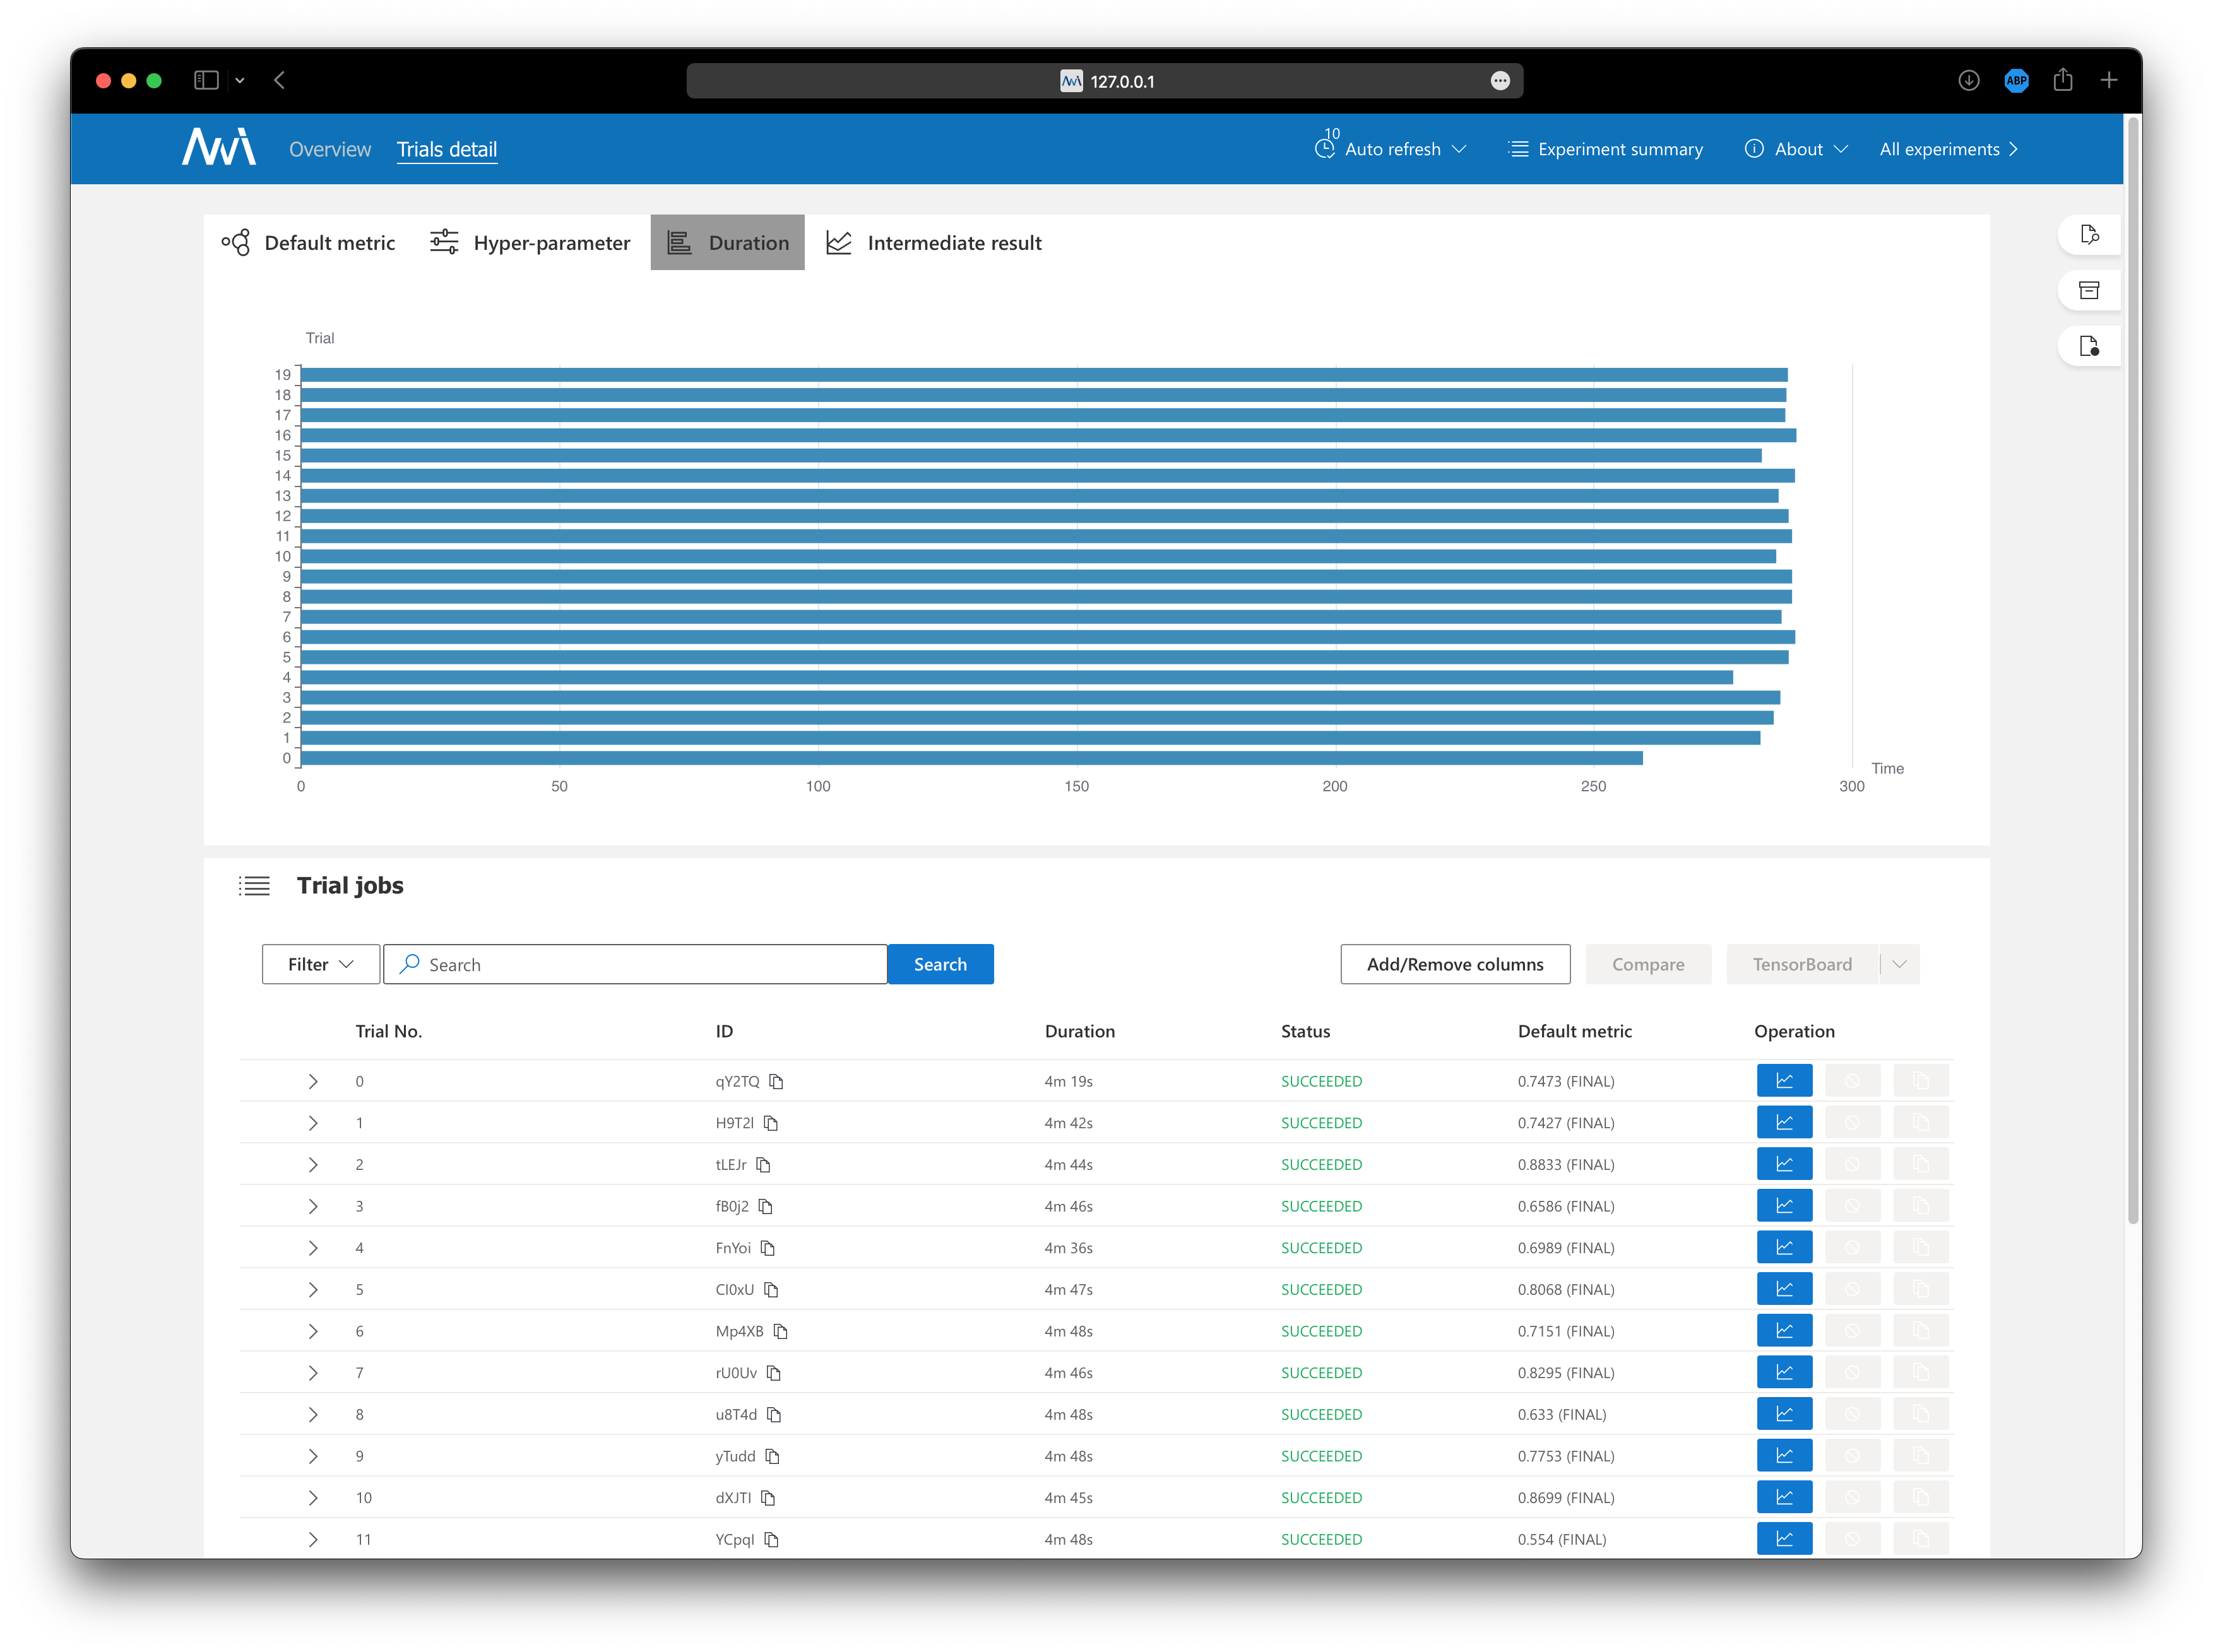
\includegraphics[width=3.5in]{../proj3/figures/mlp_hyperband_latency.png}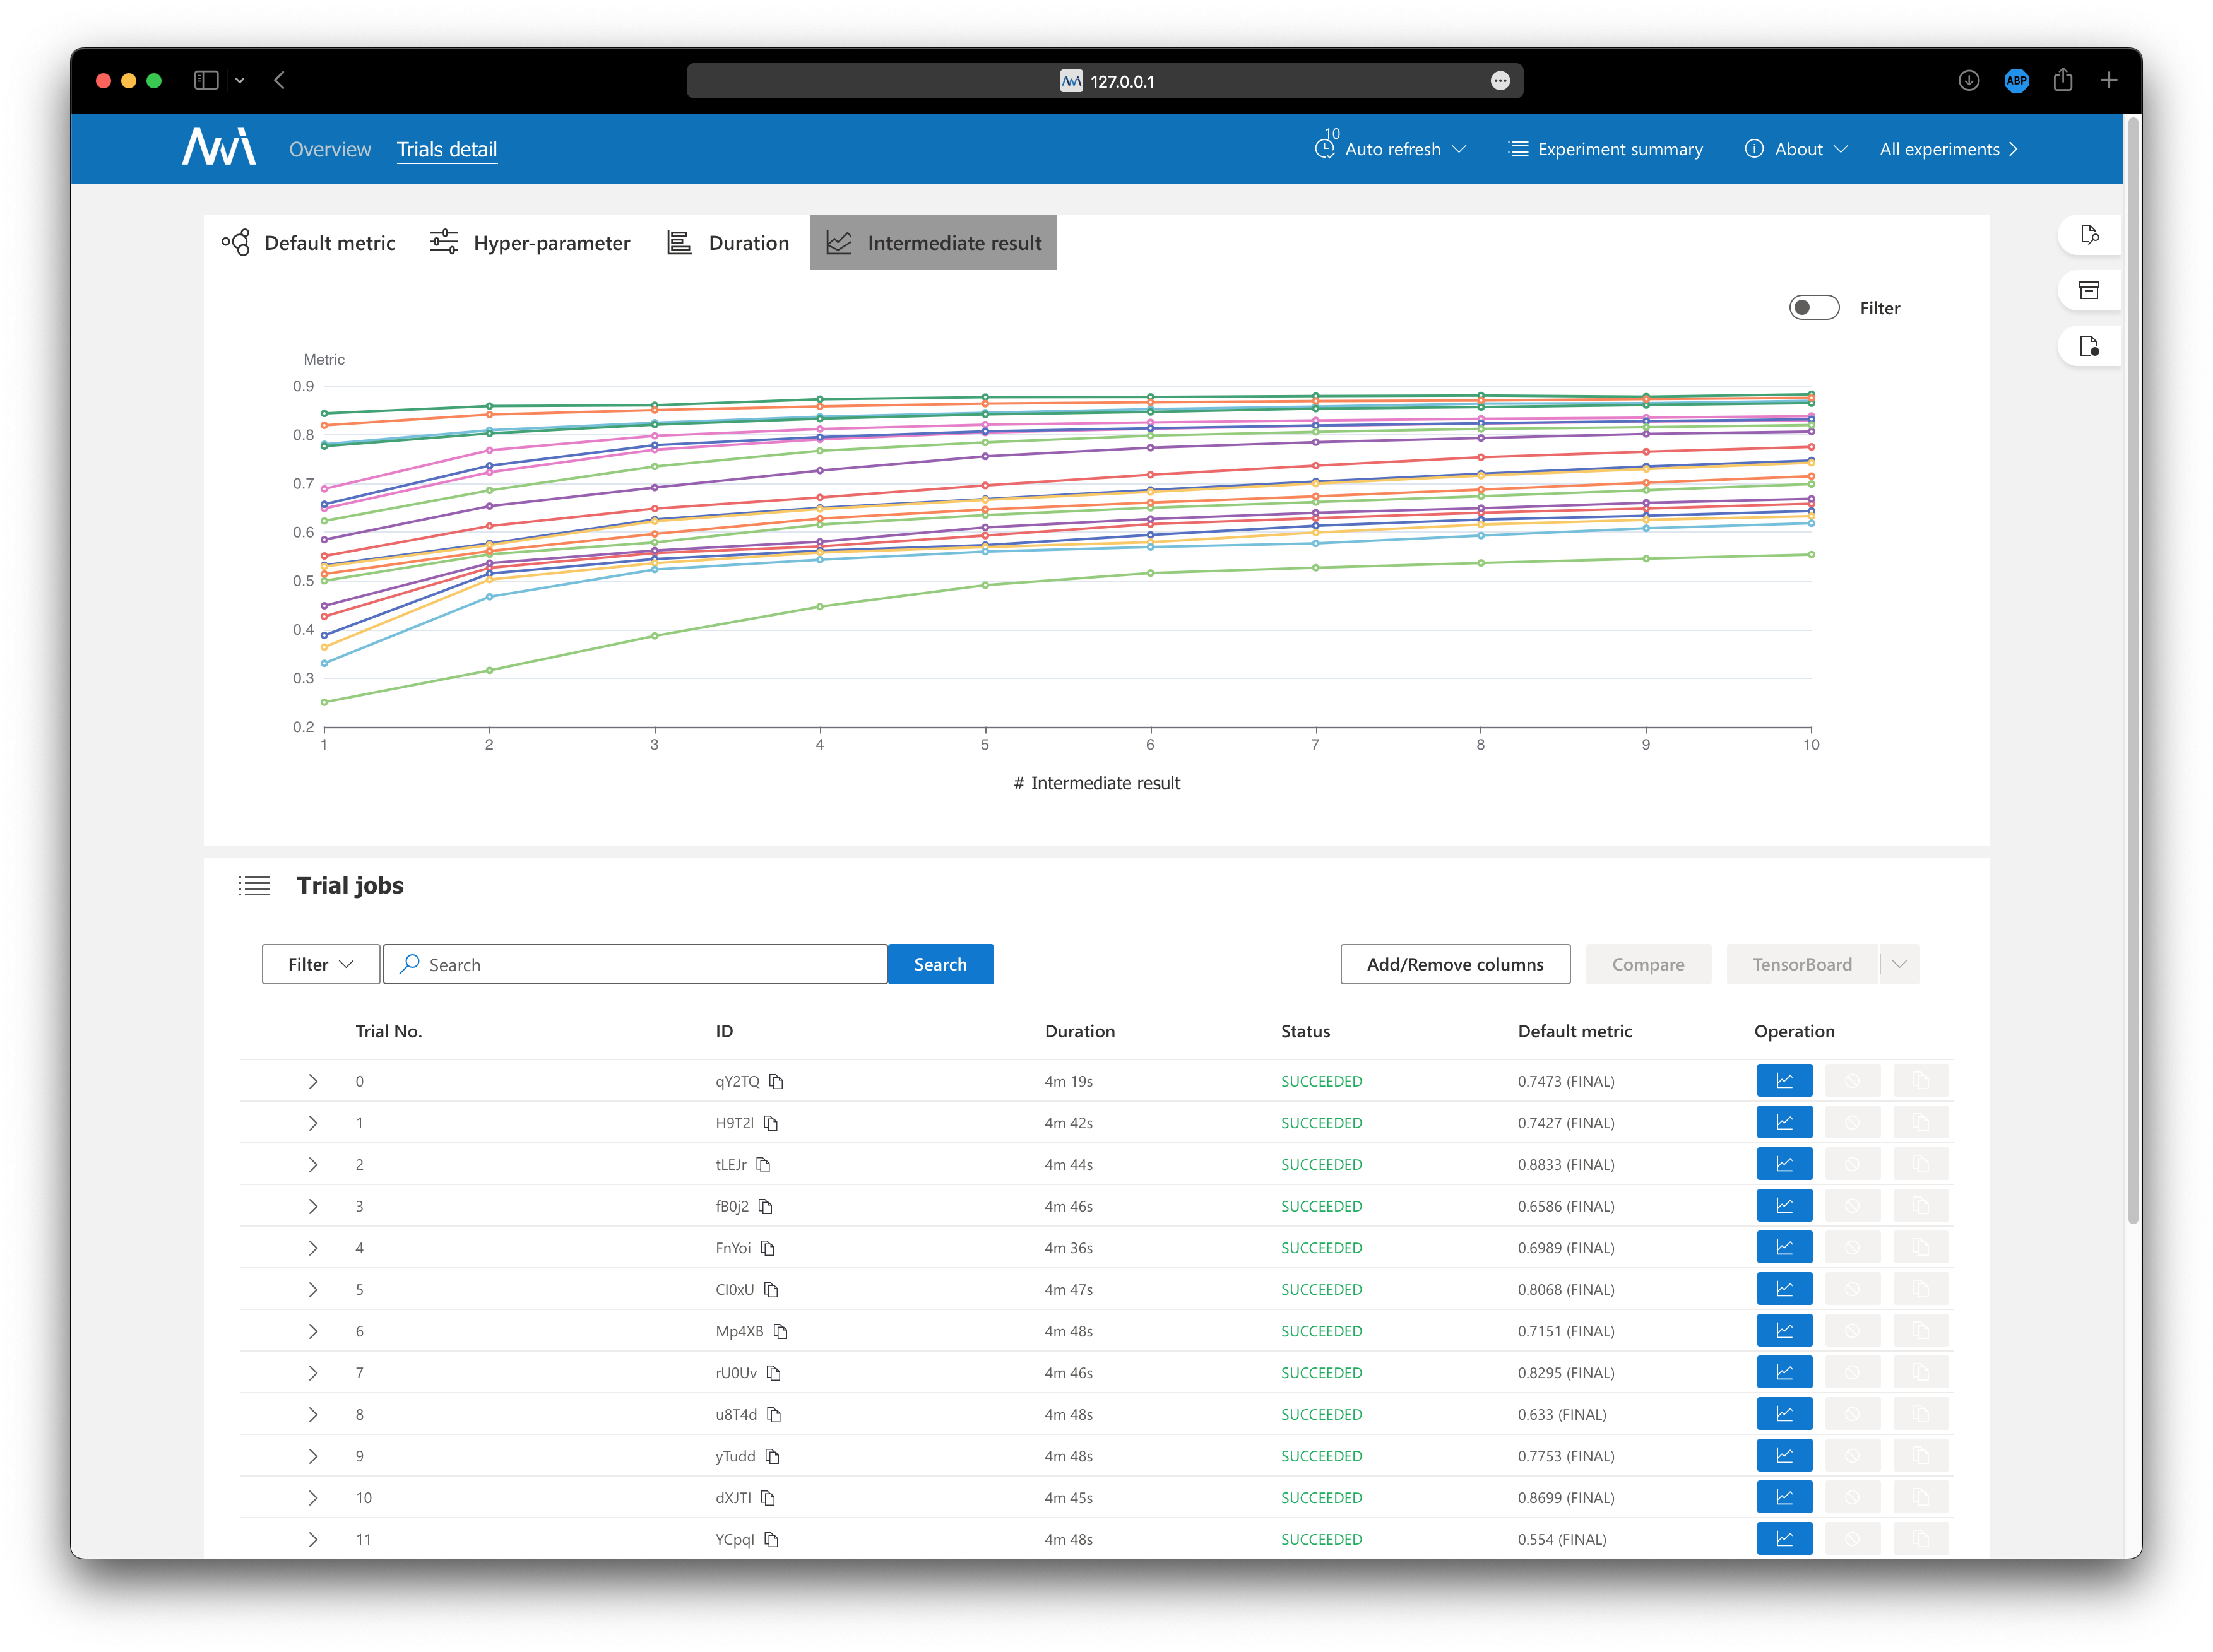
\includegraphics[width=3.5in]{../proj3/figures/mlp_hyperband_intermediate.png}}
    \caption{MLP with Hyperband Tuner on Learning Rate and Momentum}
    \label{fig:mlp-hyperband}
\end{figure}

For all of the tuners, there weren't any surprising differences. TPE turned out to perform the best, and all of the trials ran for the same amount of time, which makes sense as we're just tuning learning rate and momentum.

\subsection{MLP HPO Experiments with Learning Rate, Momentum, Feature Size, and Batch Size}

Figure \ref{fig:mlp-tpe-batch} shows the result of the MLP with TPE. We observe that Trial 6 has the most optimal parameters with a validation accuracy of 88.26\%. The optimal parameters for this trial are a learning rate of $0.0476$ and a momentum of $0.4535$. The optimal batch size is 32 and the number of features is 512. Duration for each trial ranged from 4-24 minutes. Trial 6 had a execution time of 5:43.

\begin{figure}
    \centerline{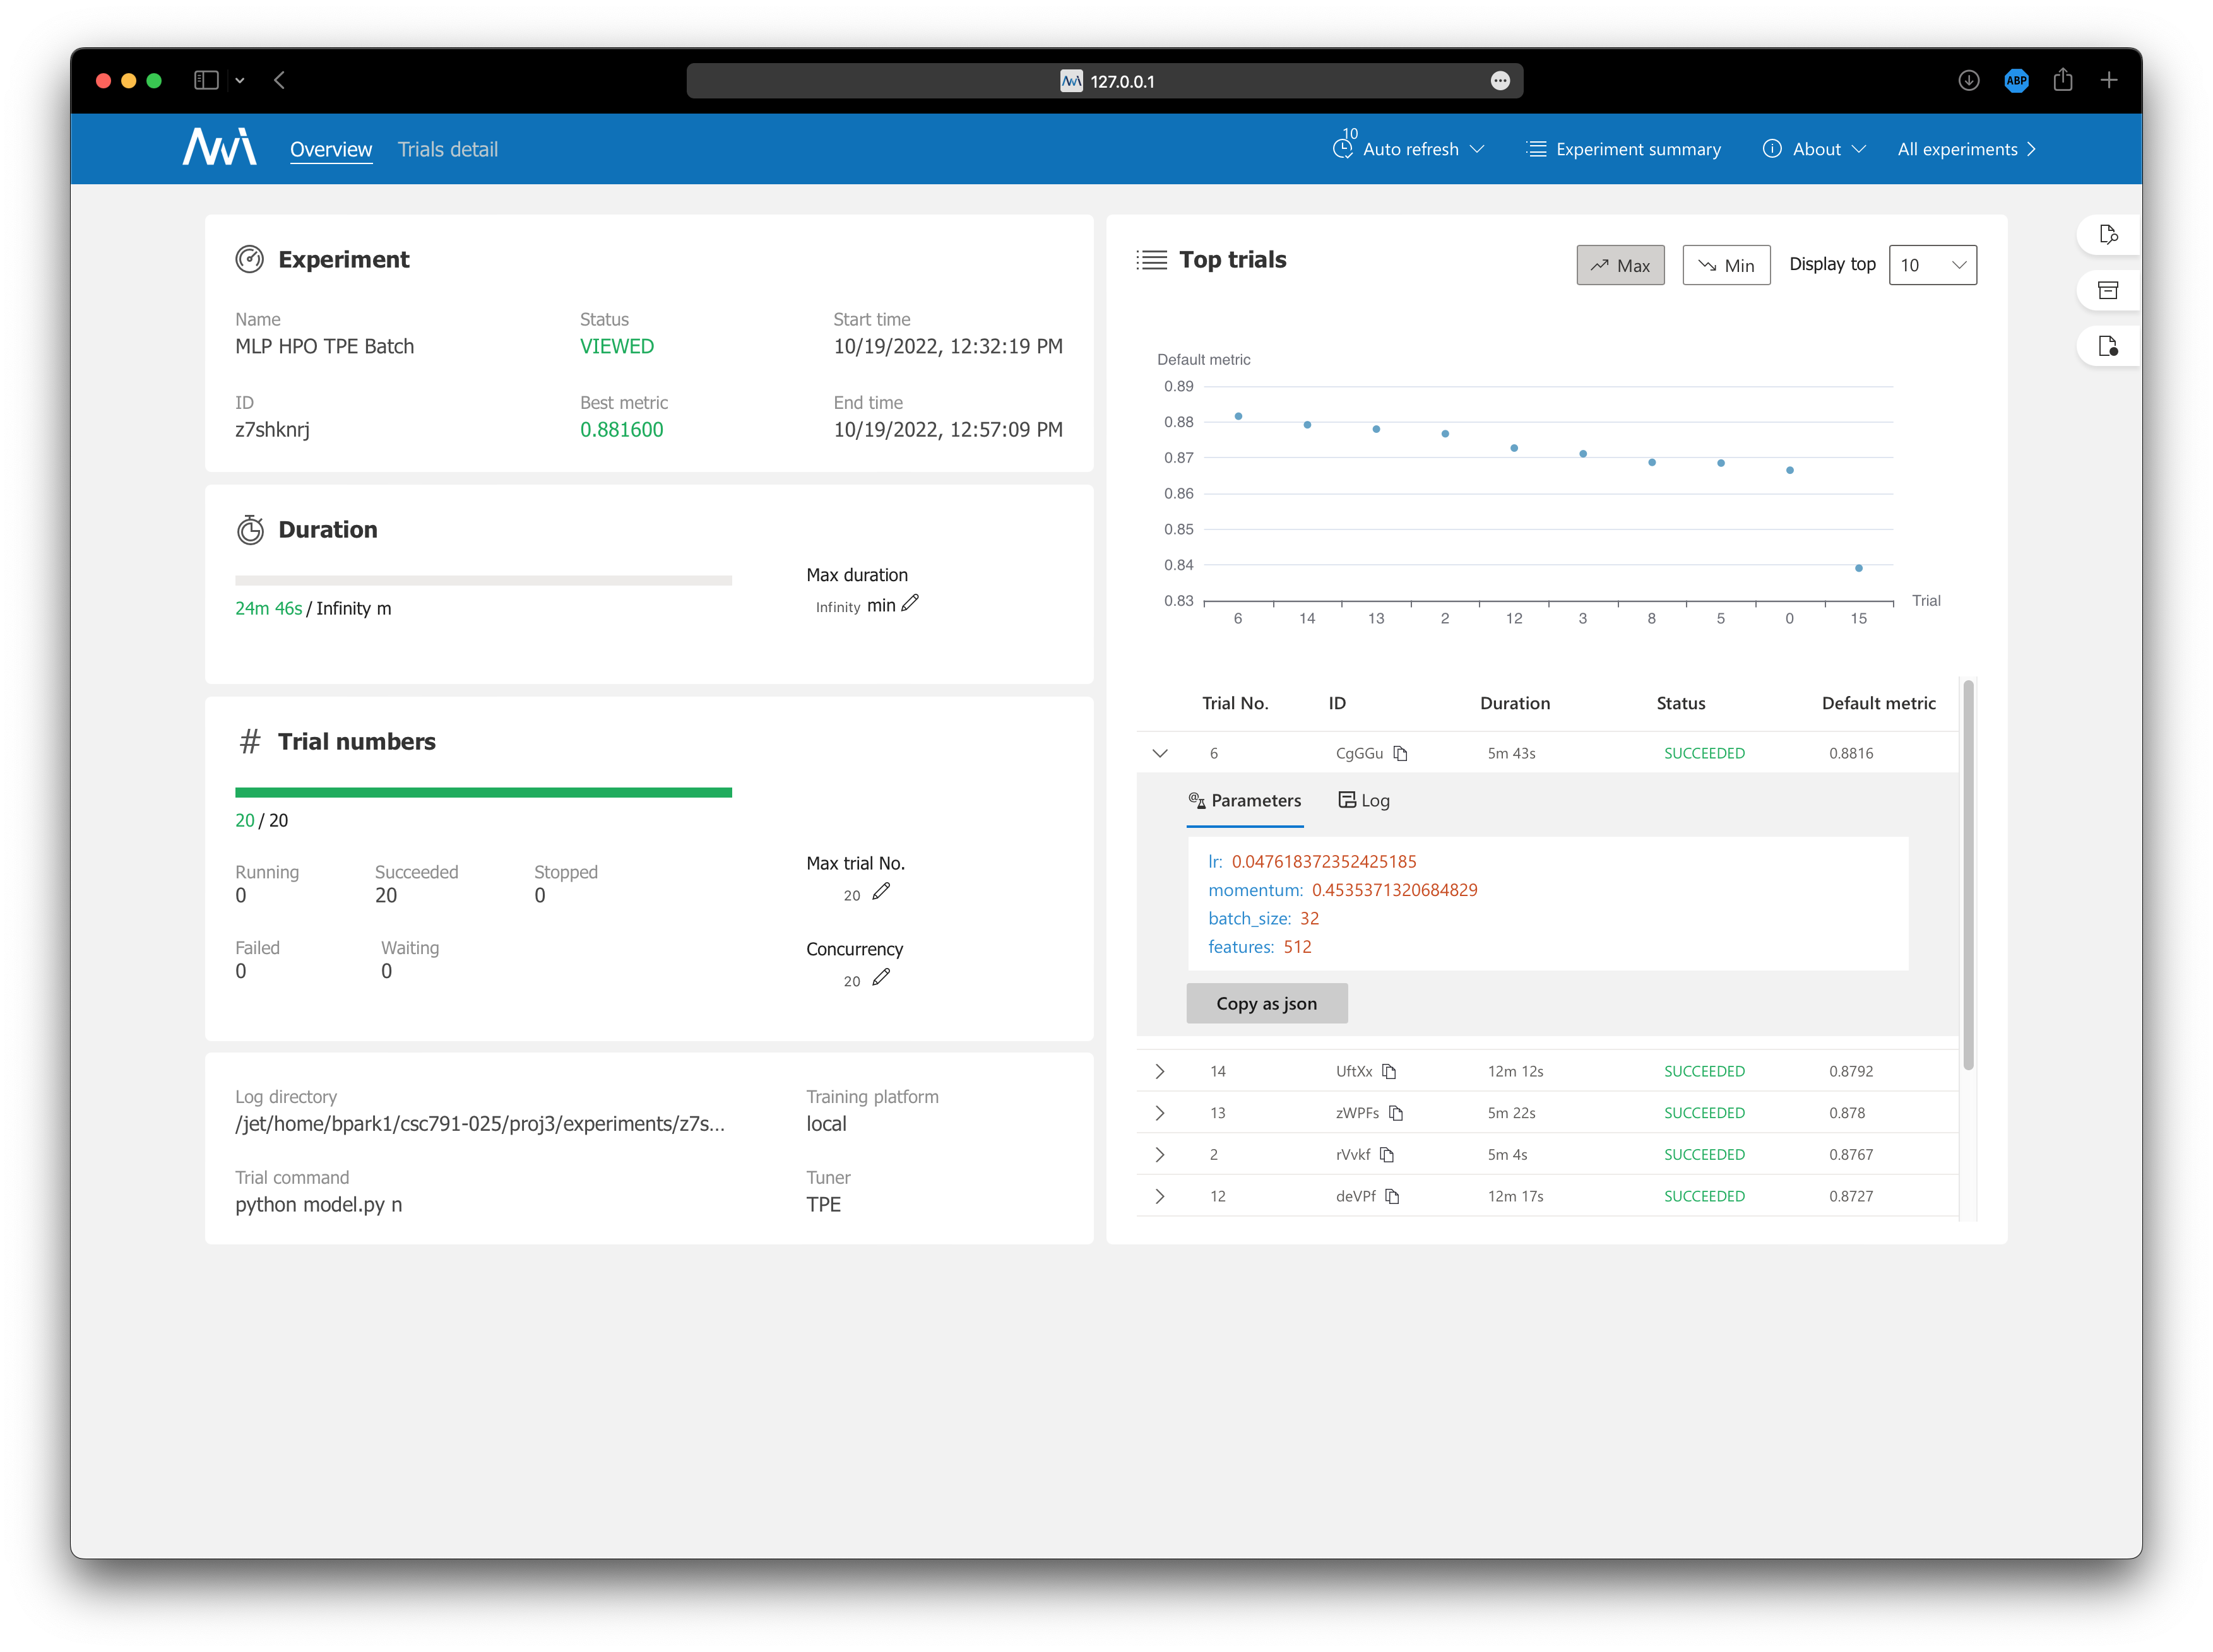
\includegraphics[width=3.5in]{../proj3/figures/mlp_tpe_batch_overview.png}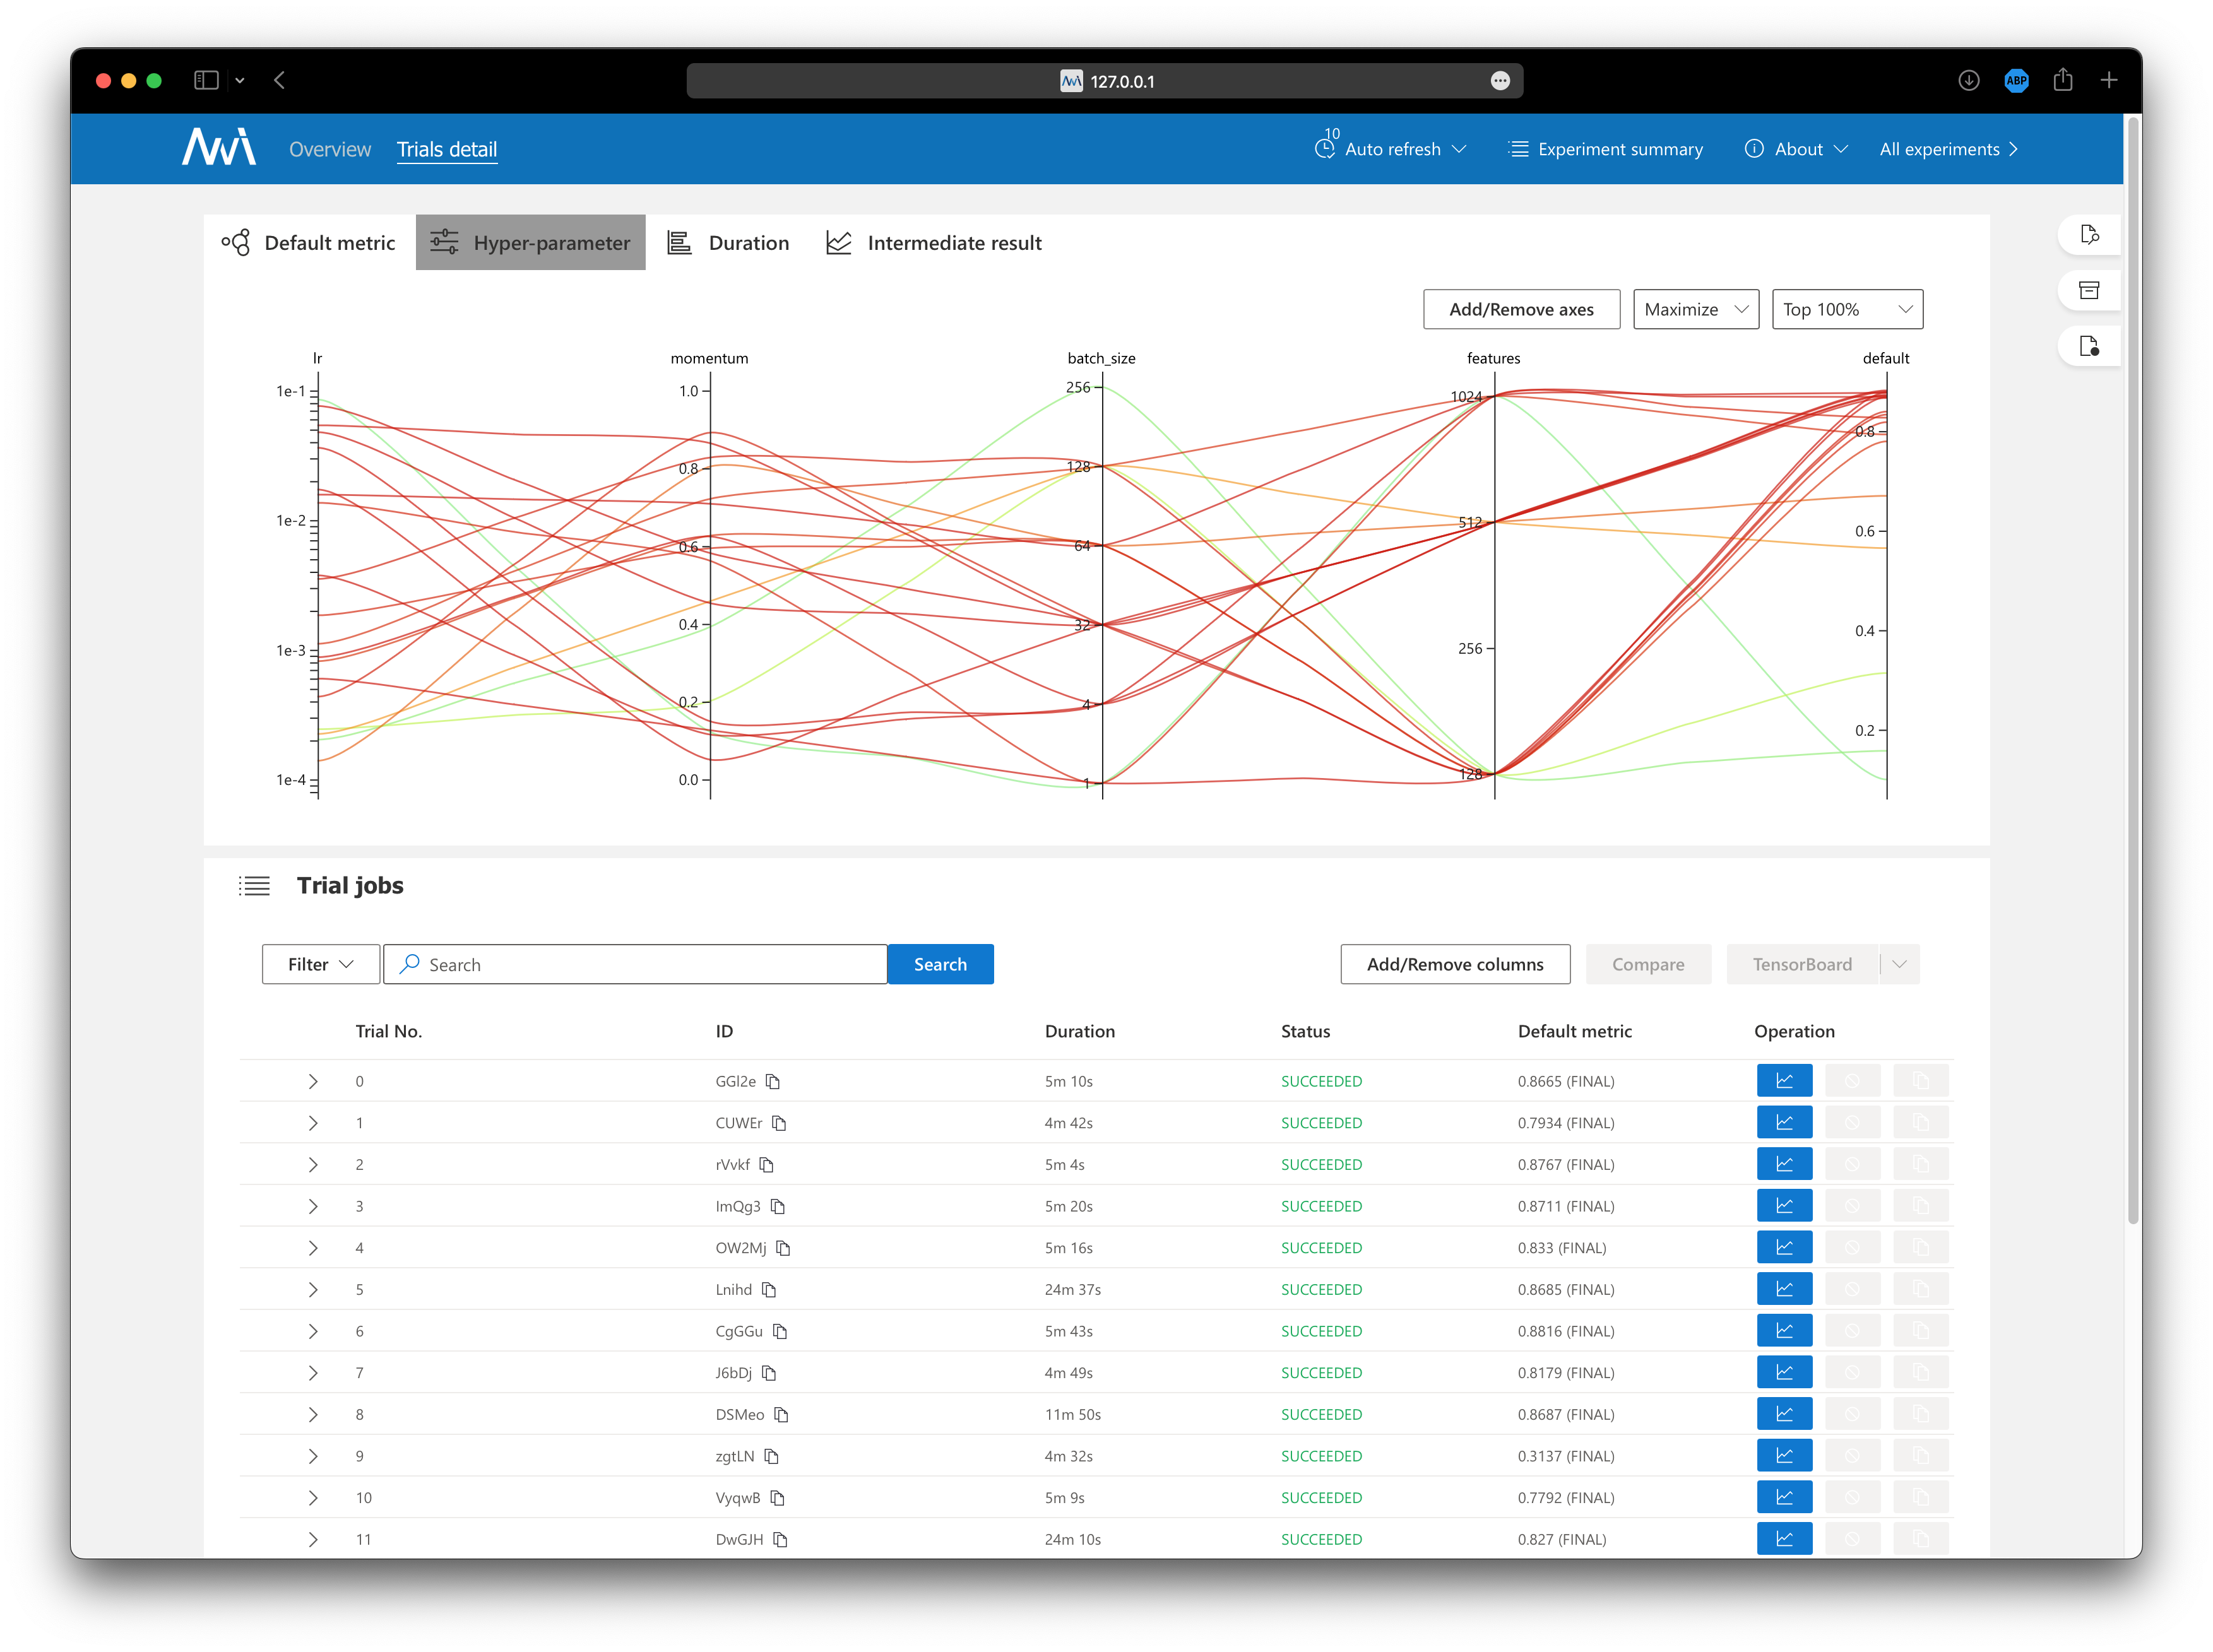
\includegraphics[width=3.5in]{../proj3/figures/mlp_tpe_batch_hyperparameter.png}}
    \centerline{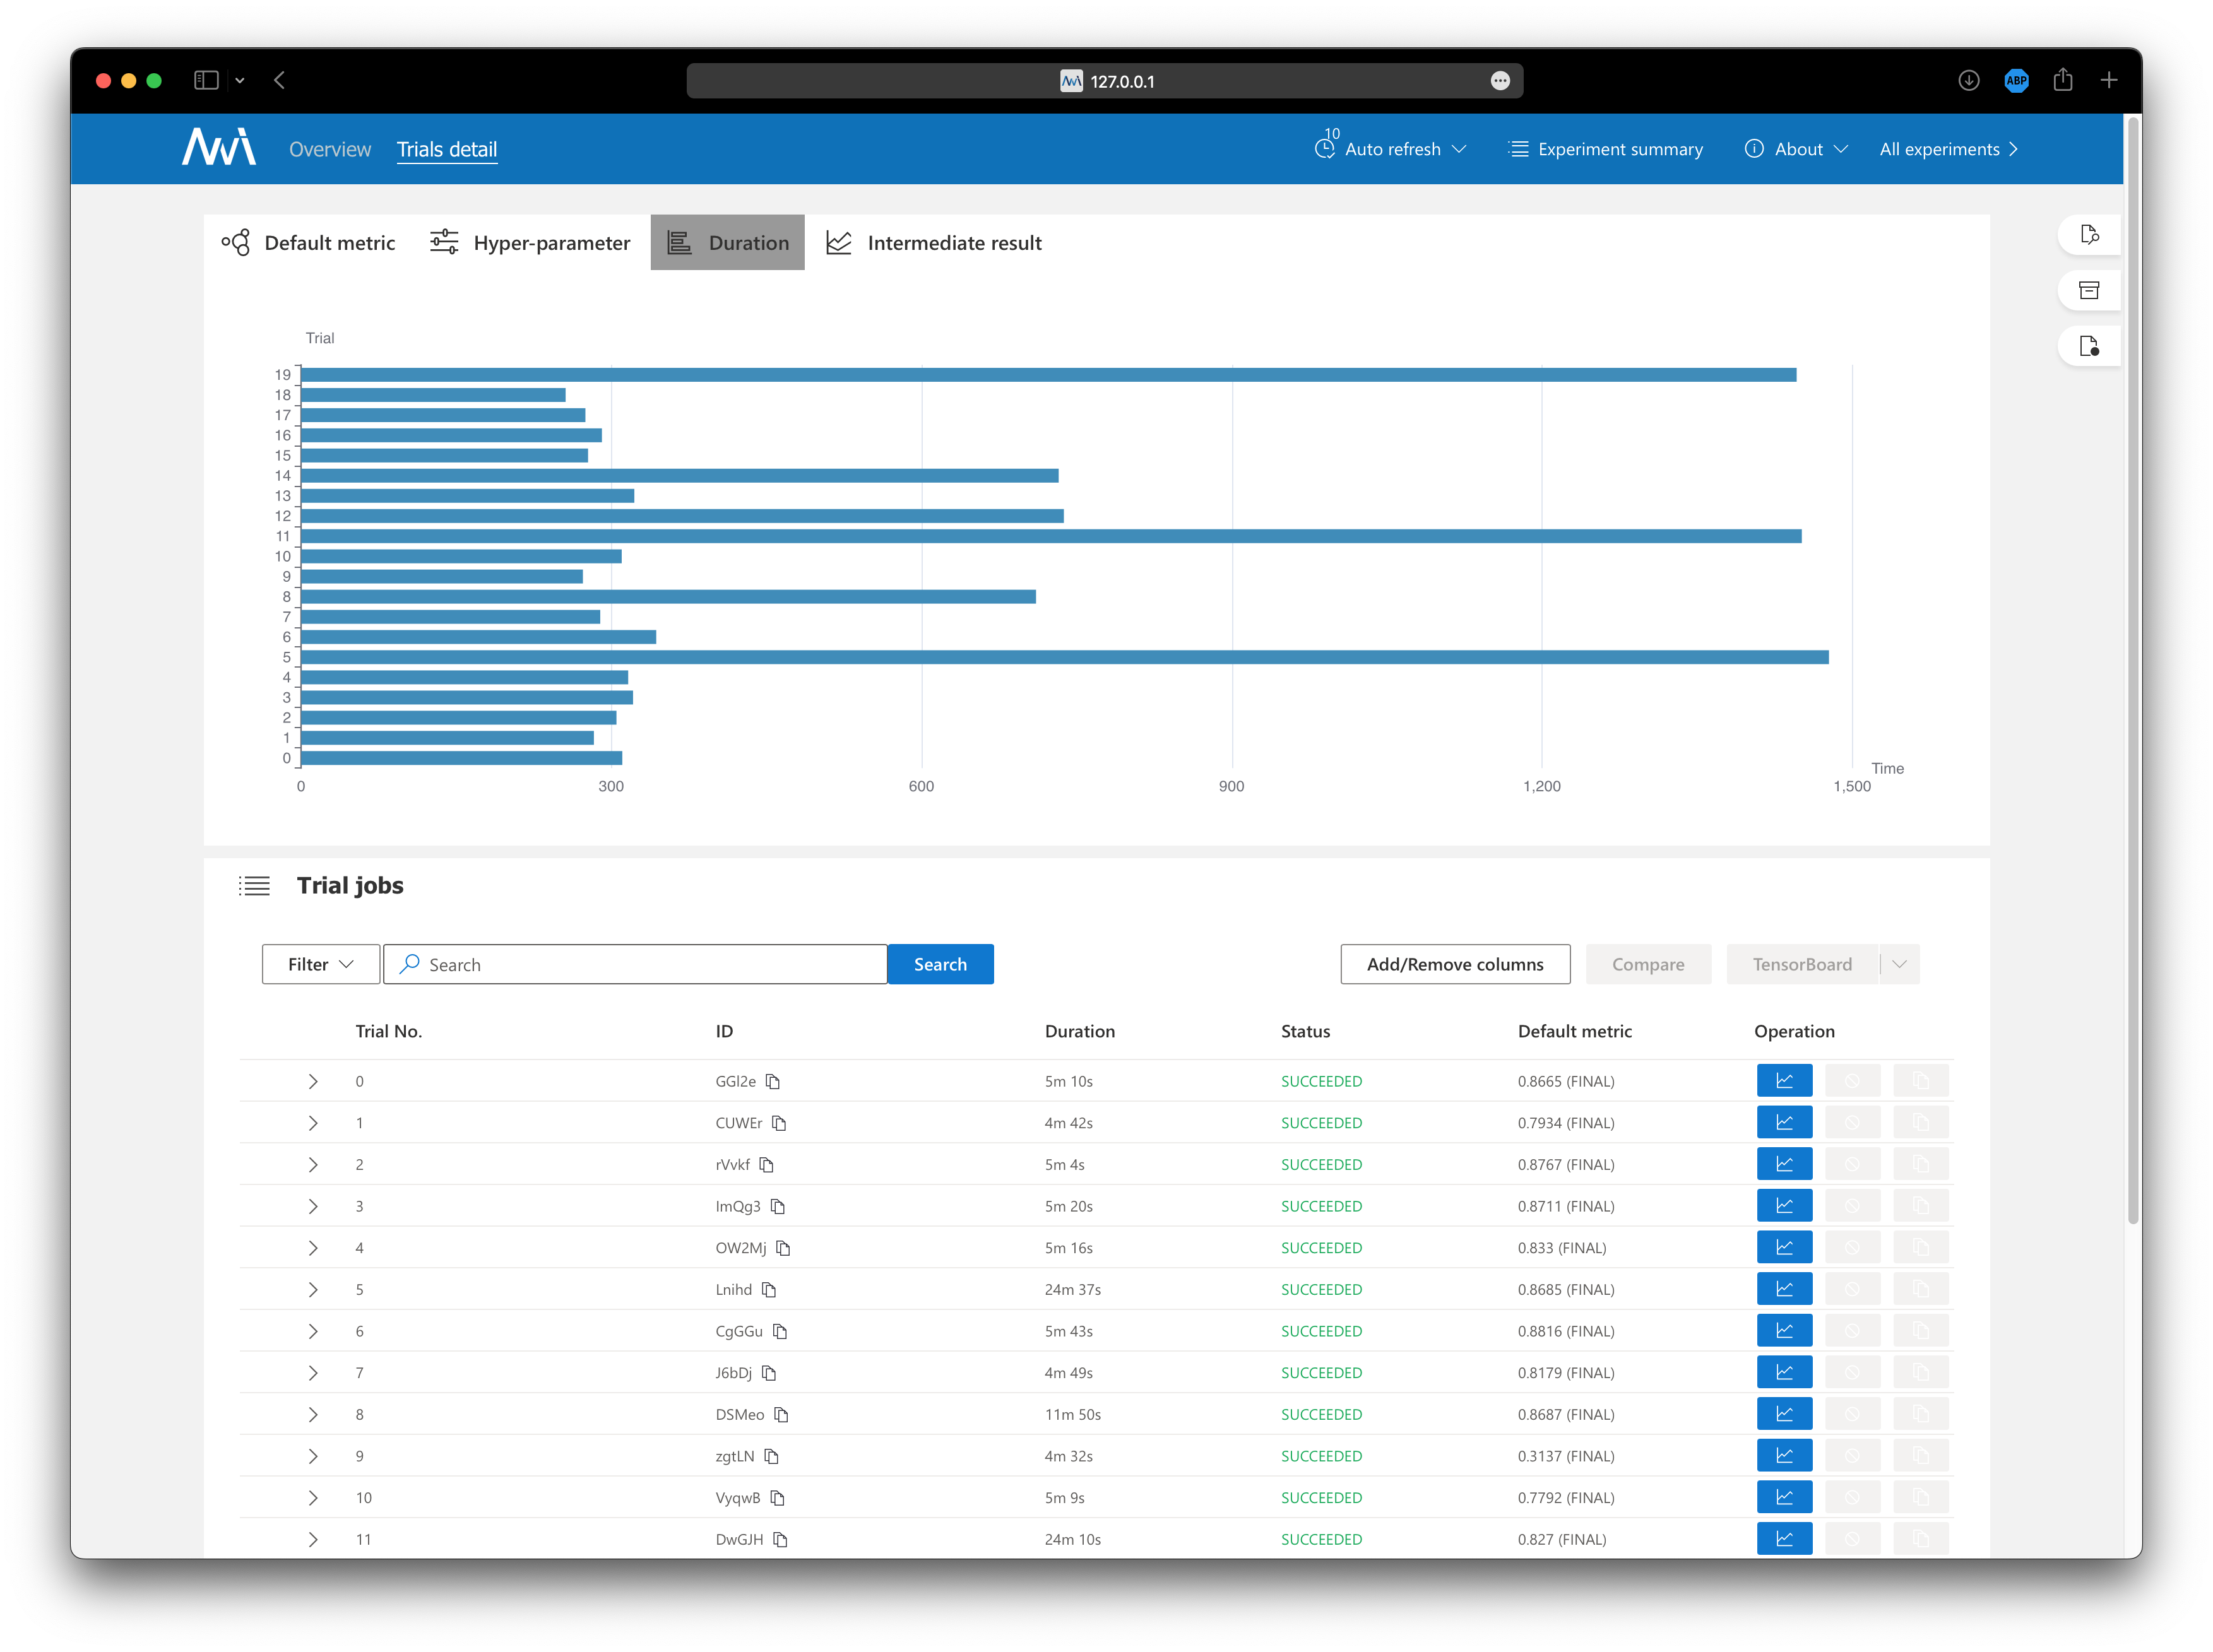
\includegraphics[width=3.5in]{../proj3/figures/mlp_tpe_batch_latency.png}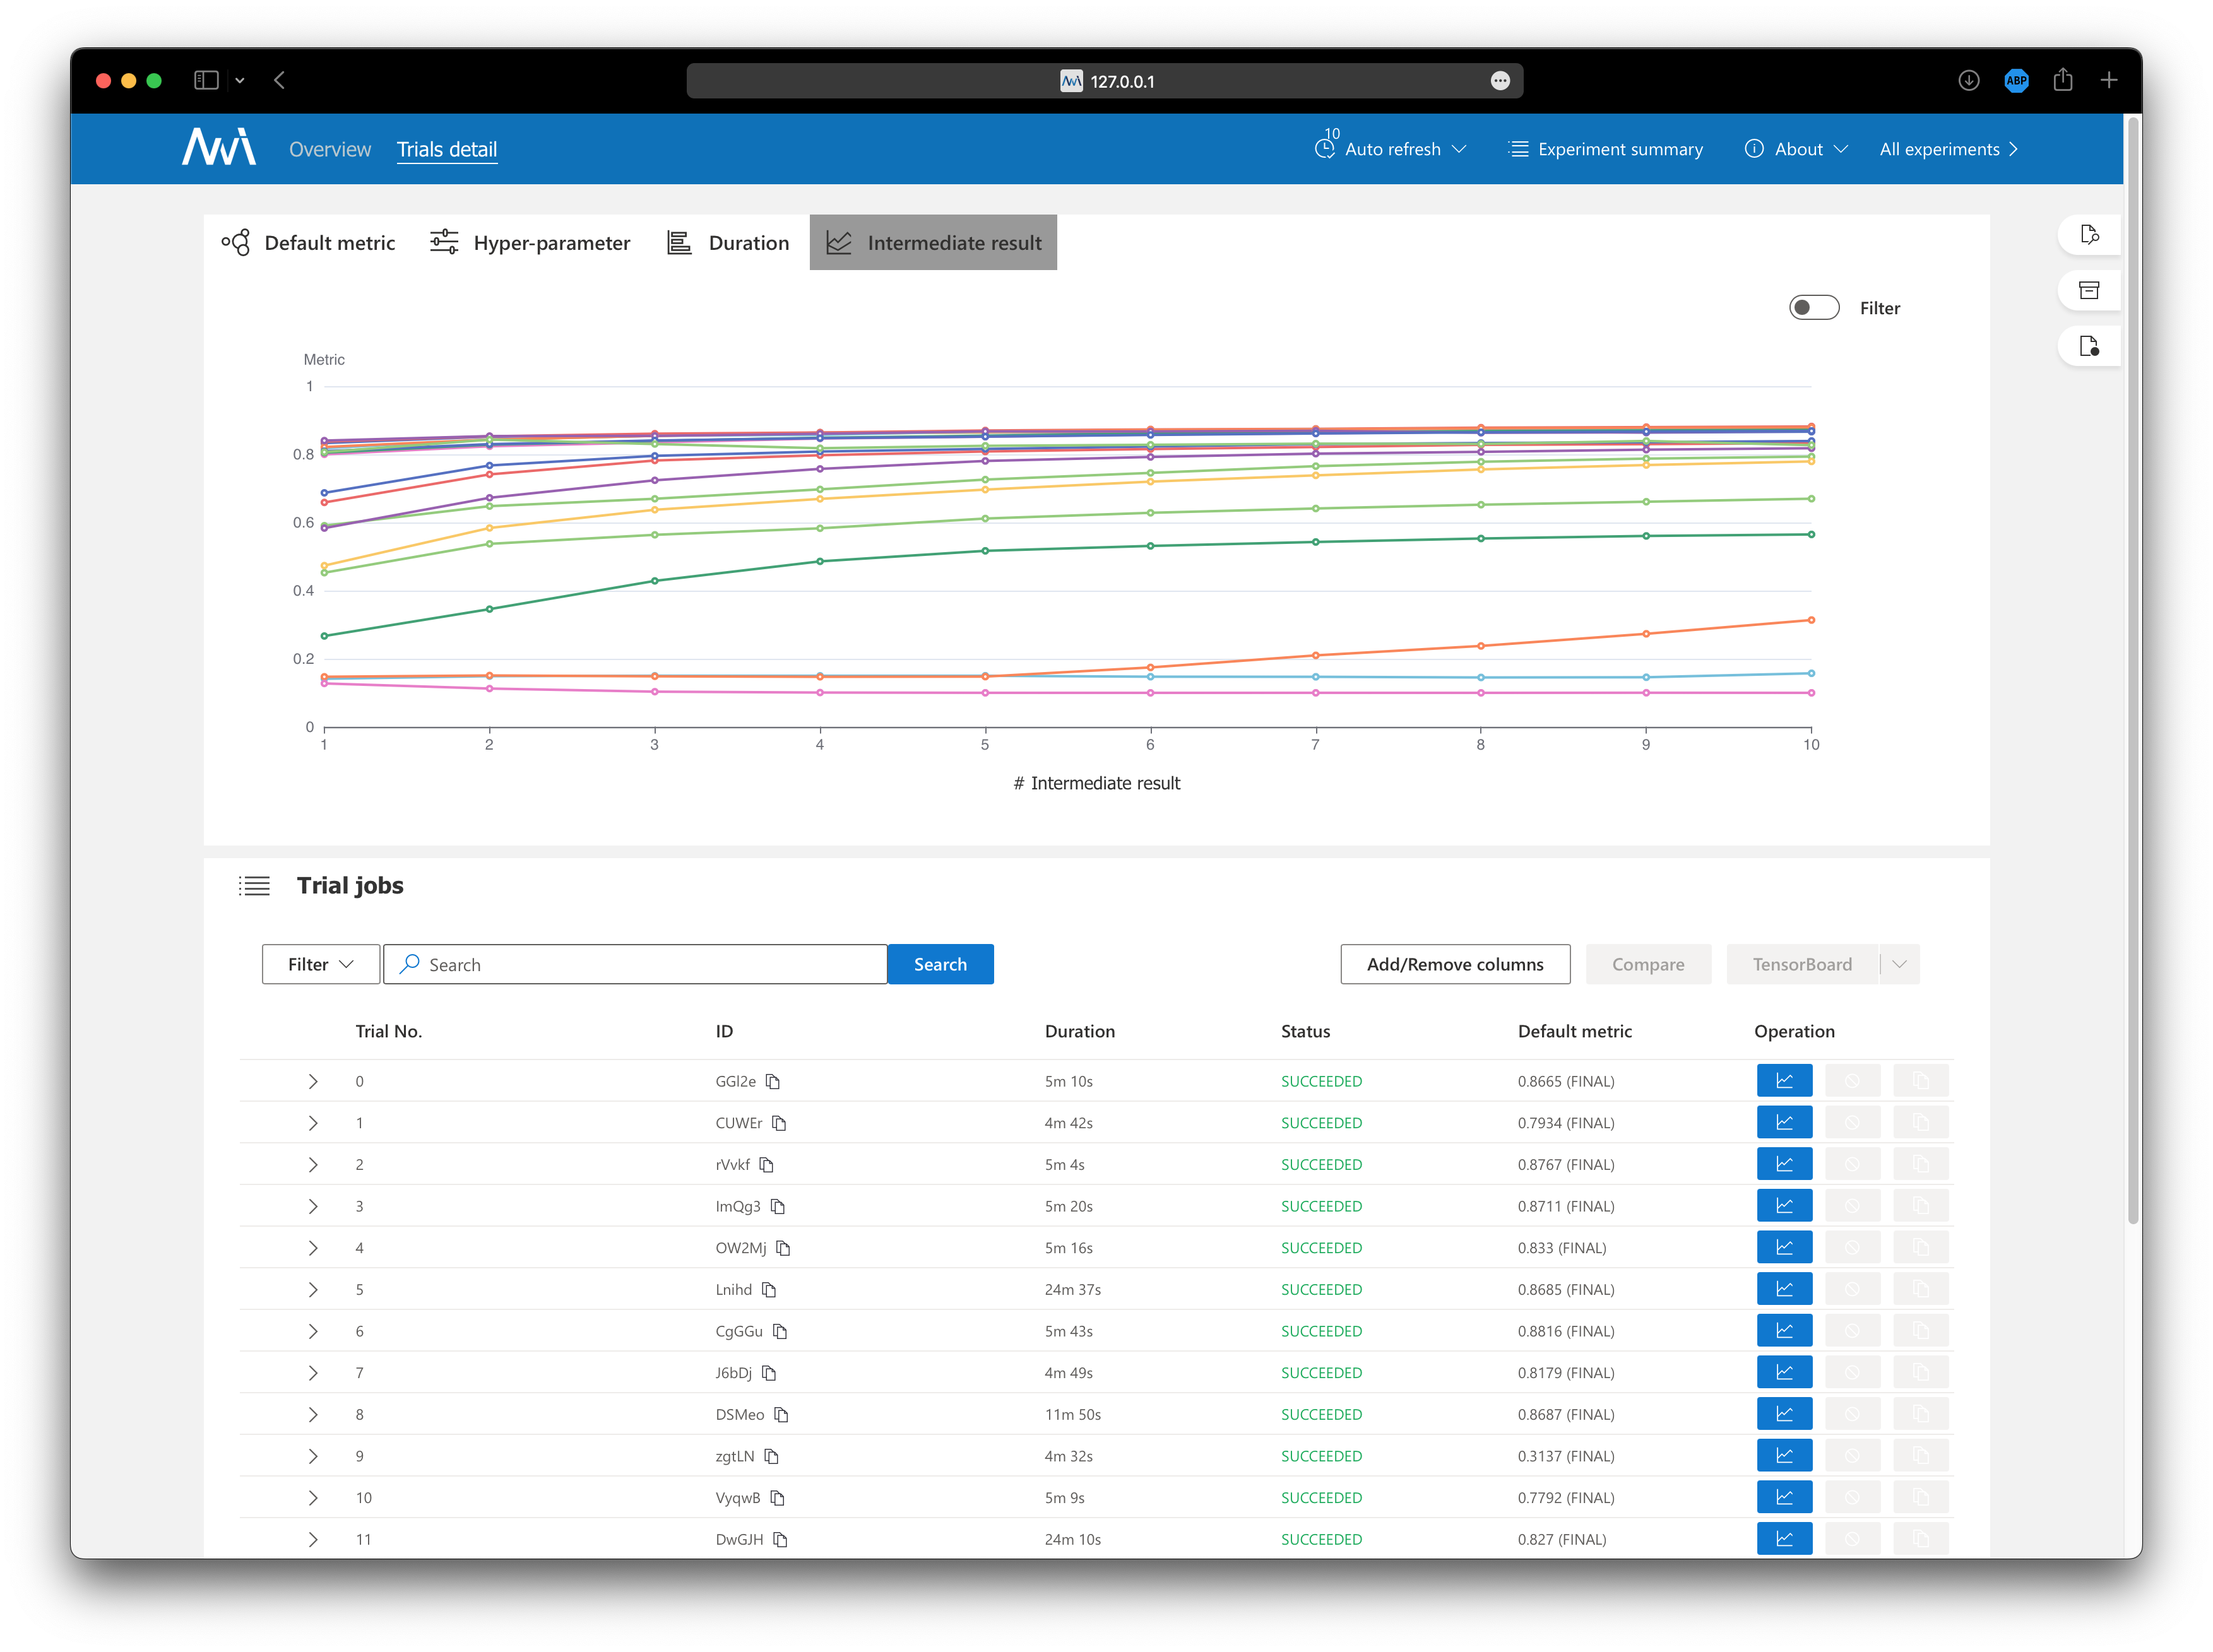
\includegraphics[width=3.5in]{../proj3/figures/mlp_tpe_batch_intermediate.png}}
    \caption{MLP with TPE Tuner on Learning Rate, Momentum, Feature Size, and Batch Size}
    \label{fig:mlp-tpe-batch}
\end{figure}

Figure \ref{fig:mlp-evolution-batch} shows the result of the MLP with Evolution. We observe that Trial 2 has the most optimal parameters with a validation accuracy of 87.98\%. The optimal parameters for this trial are a learning rate of $0.0794$ and a momentum of $0.4306$. The optimal batch size is 32 and the number of features is 512. Duration for each trial ranged from 4-21 minutes. Trial 2 had a execution time of 5:01.

\begin{figure}
    \centerline{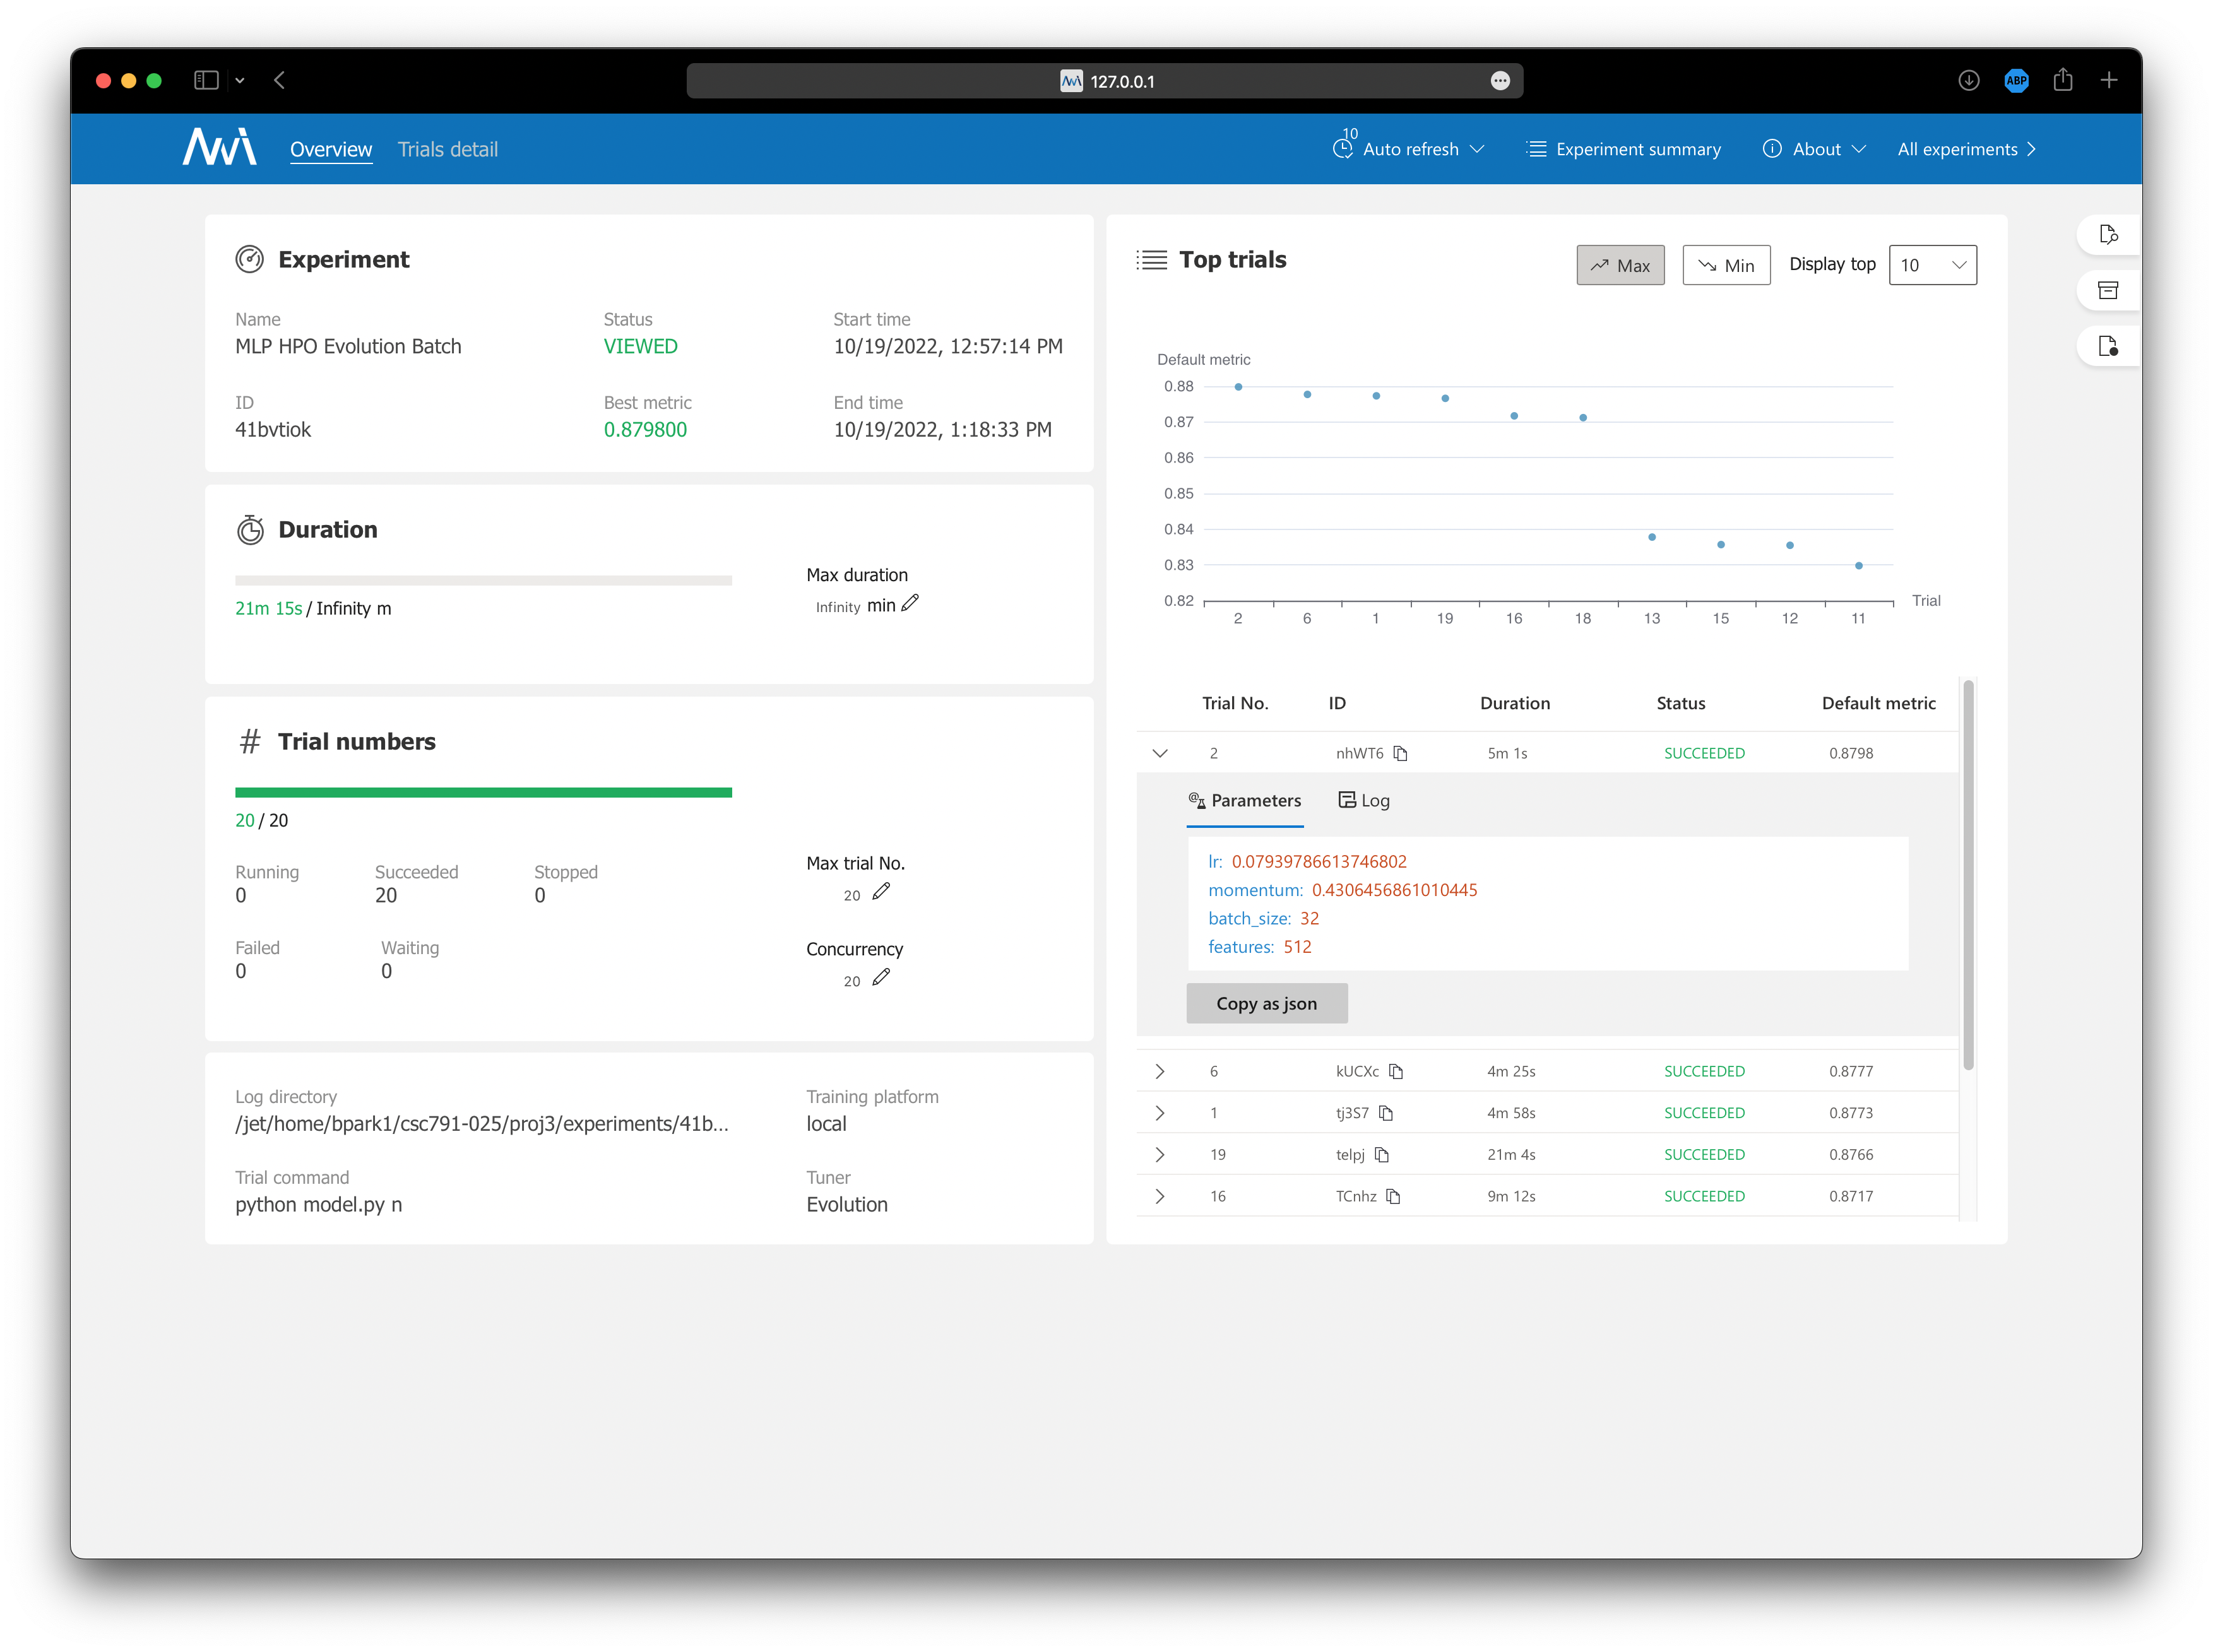
\includegraphics[width=3.5in]{../proj3/figures/mlp_evolution_batch_overview.png}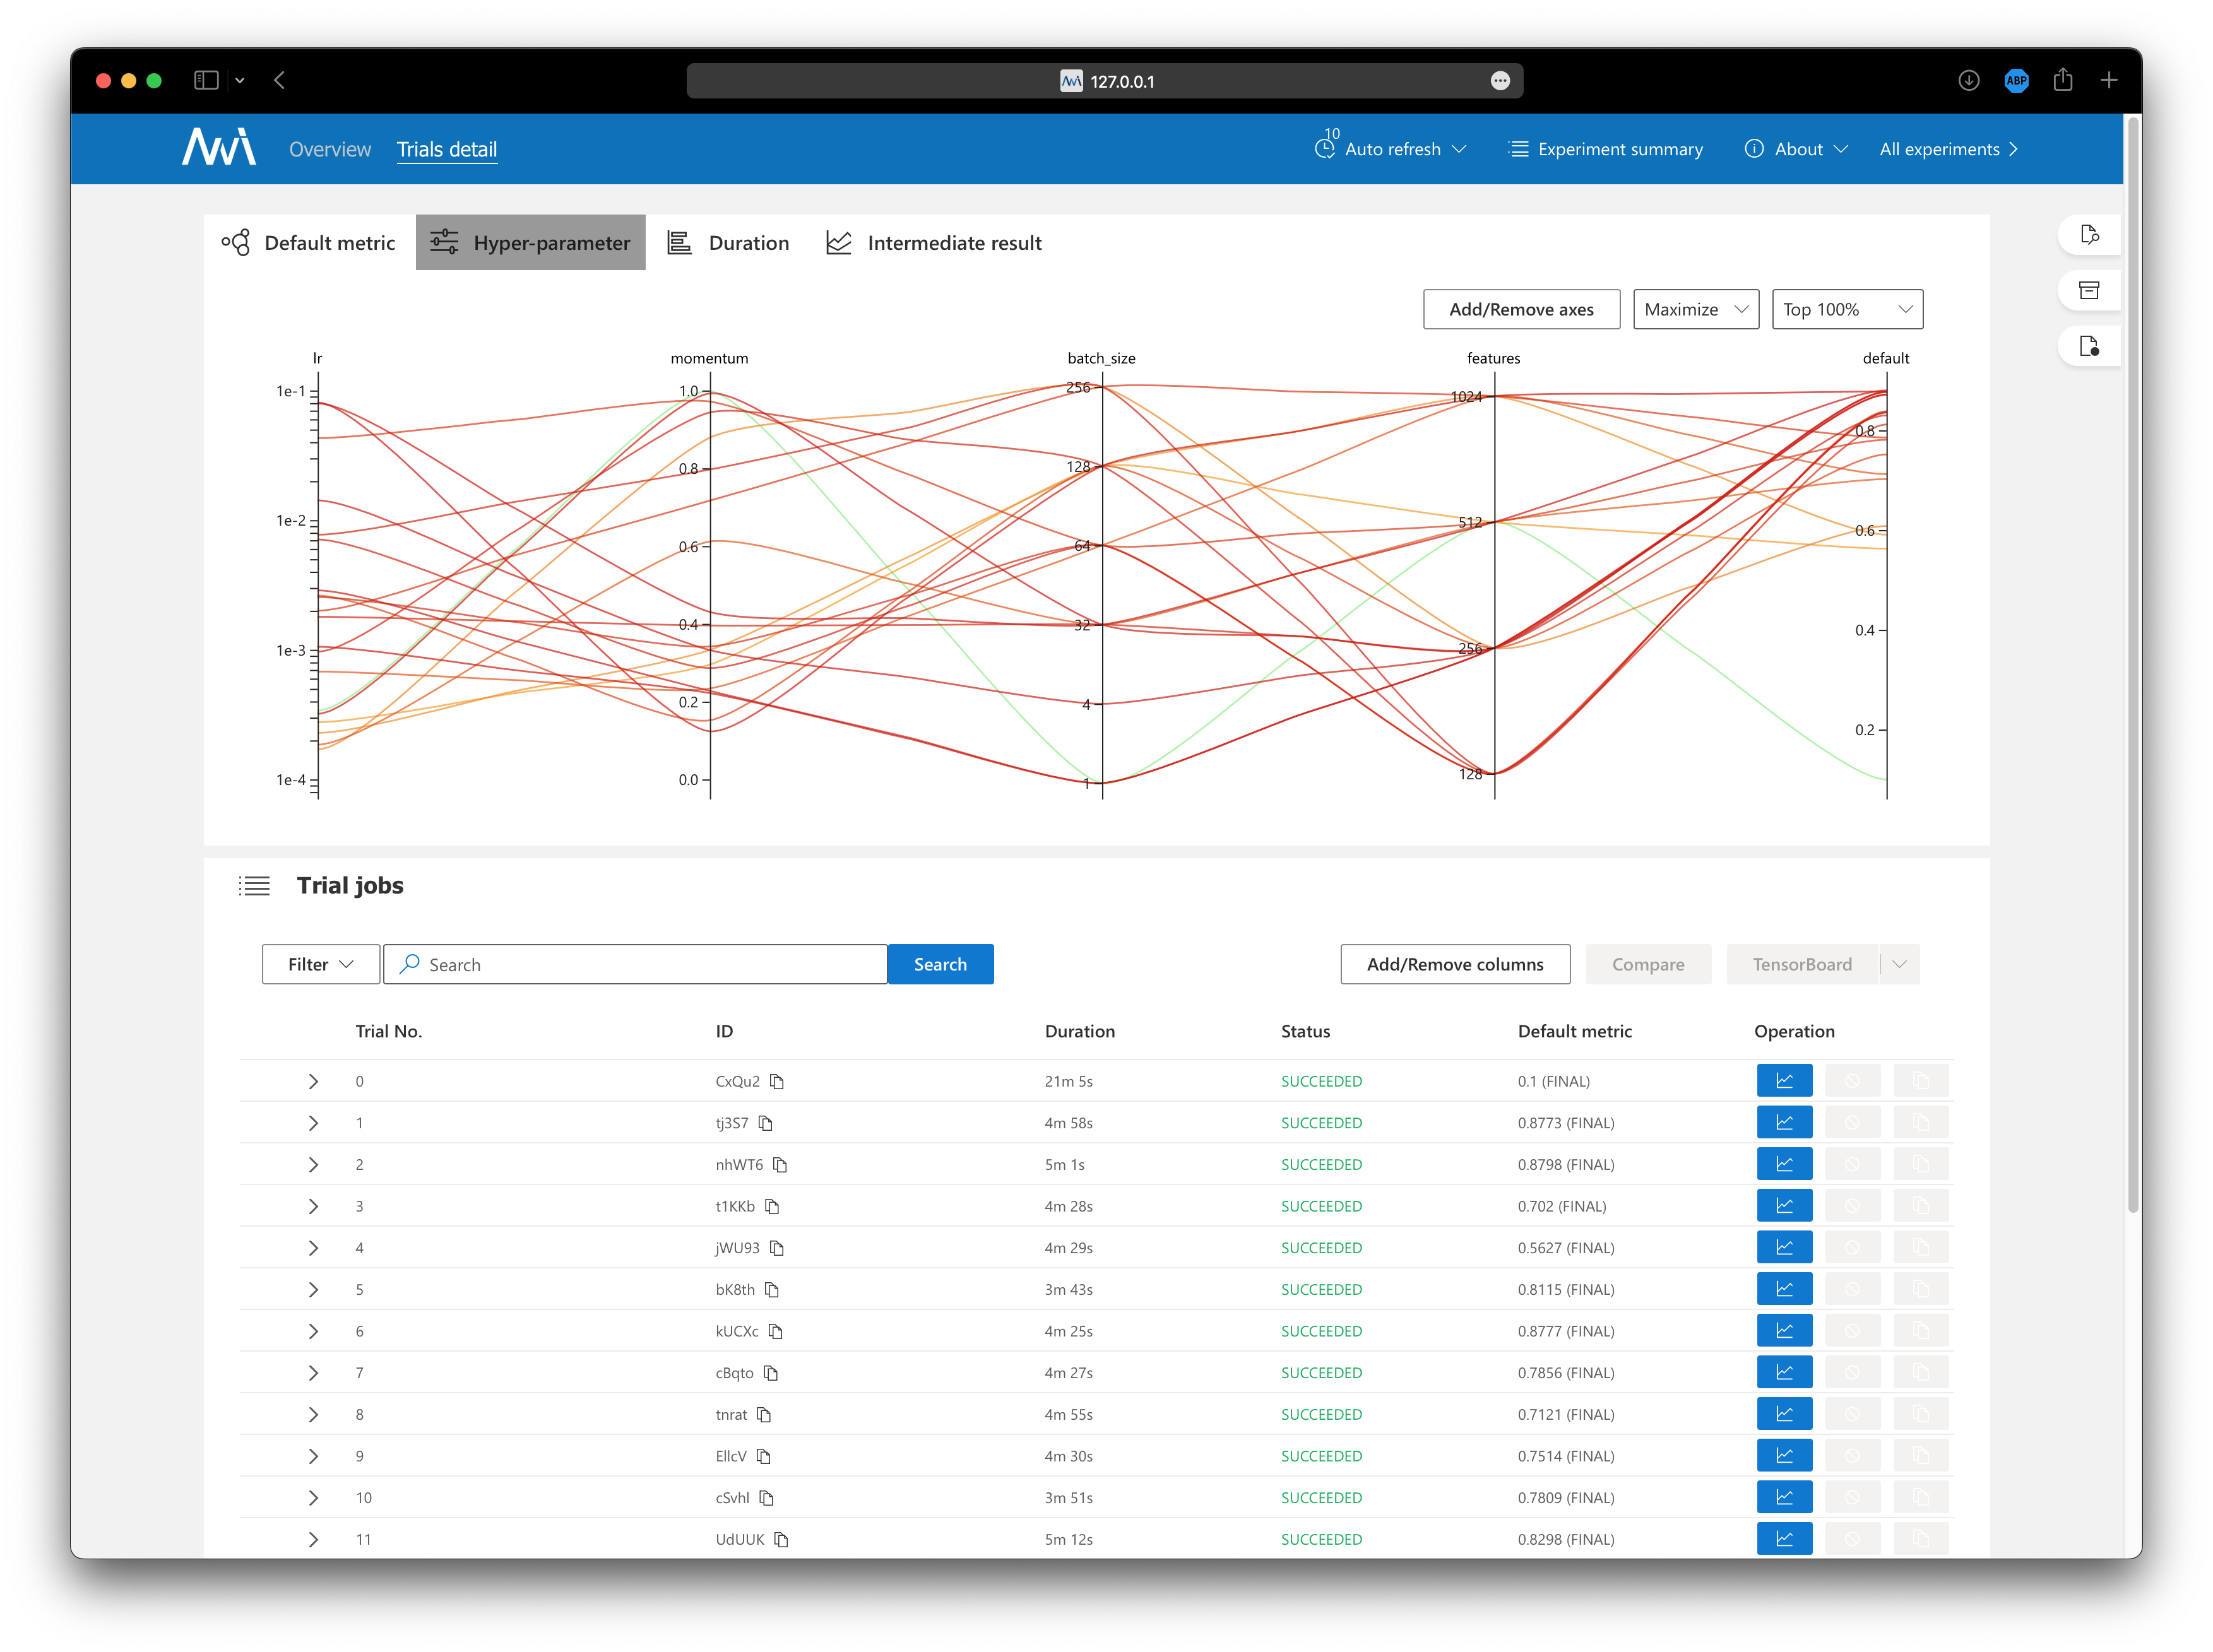
\includegraphics[width=3.5in]{../proj3/figures/mlp_evolution_batch_hyperparameter.png}}
    \centerline{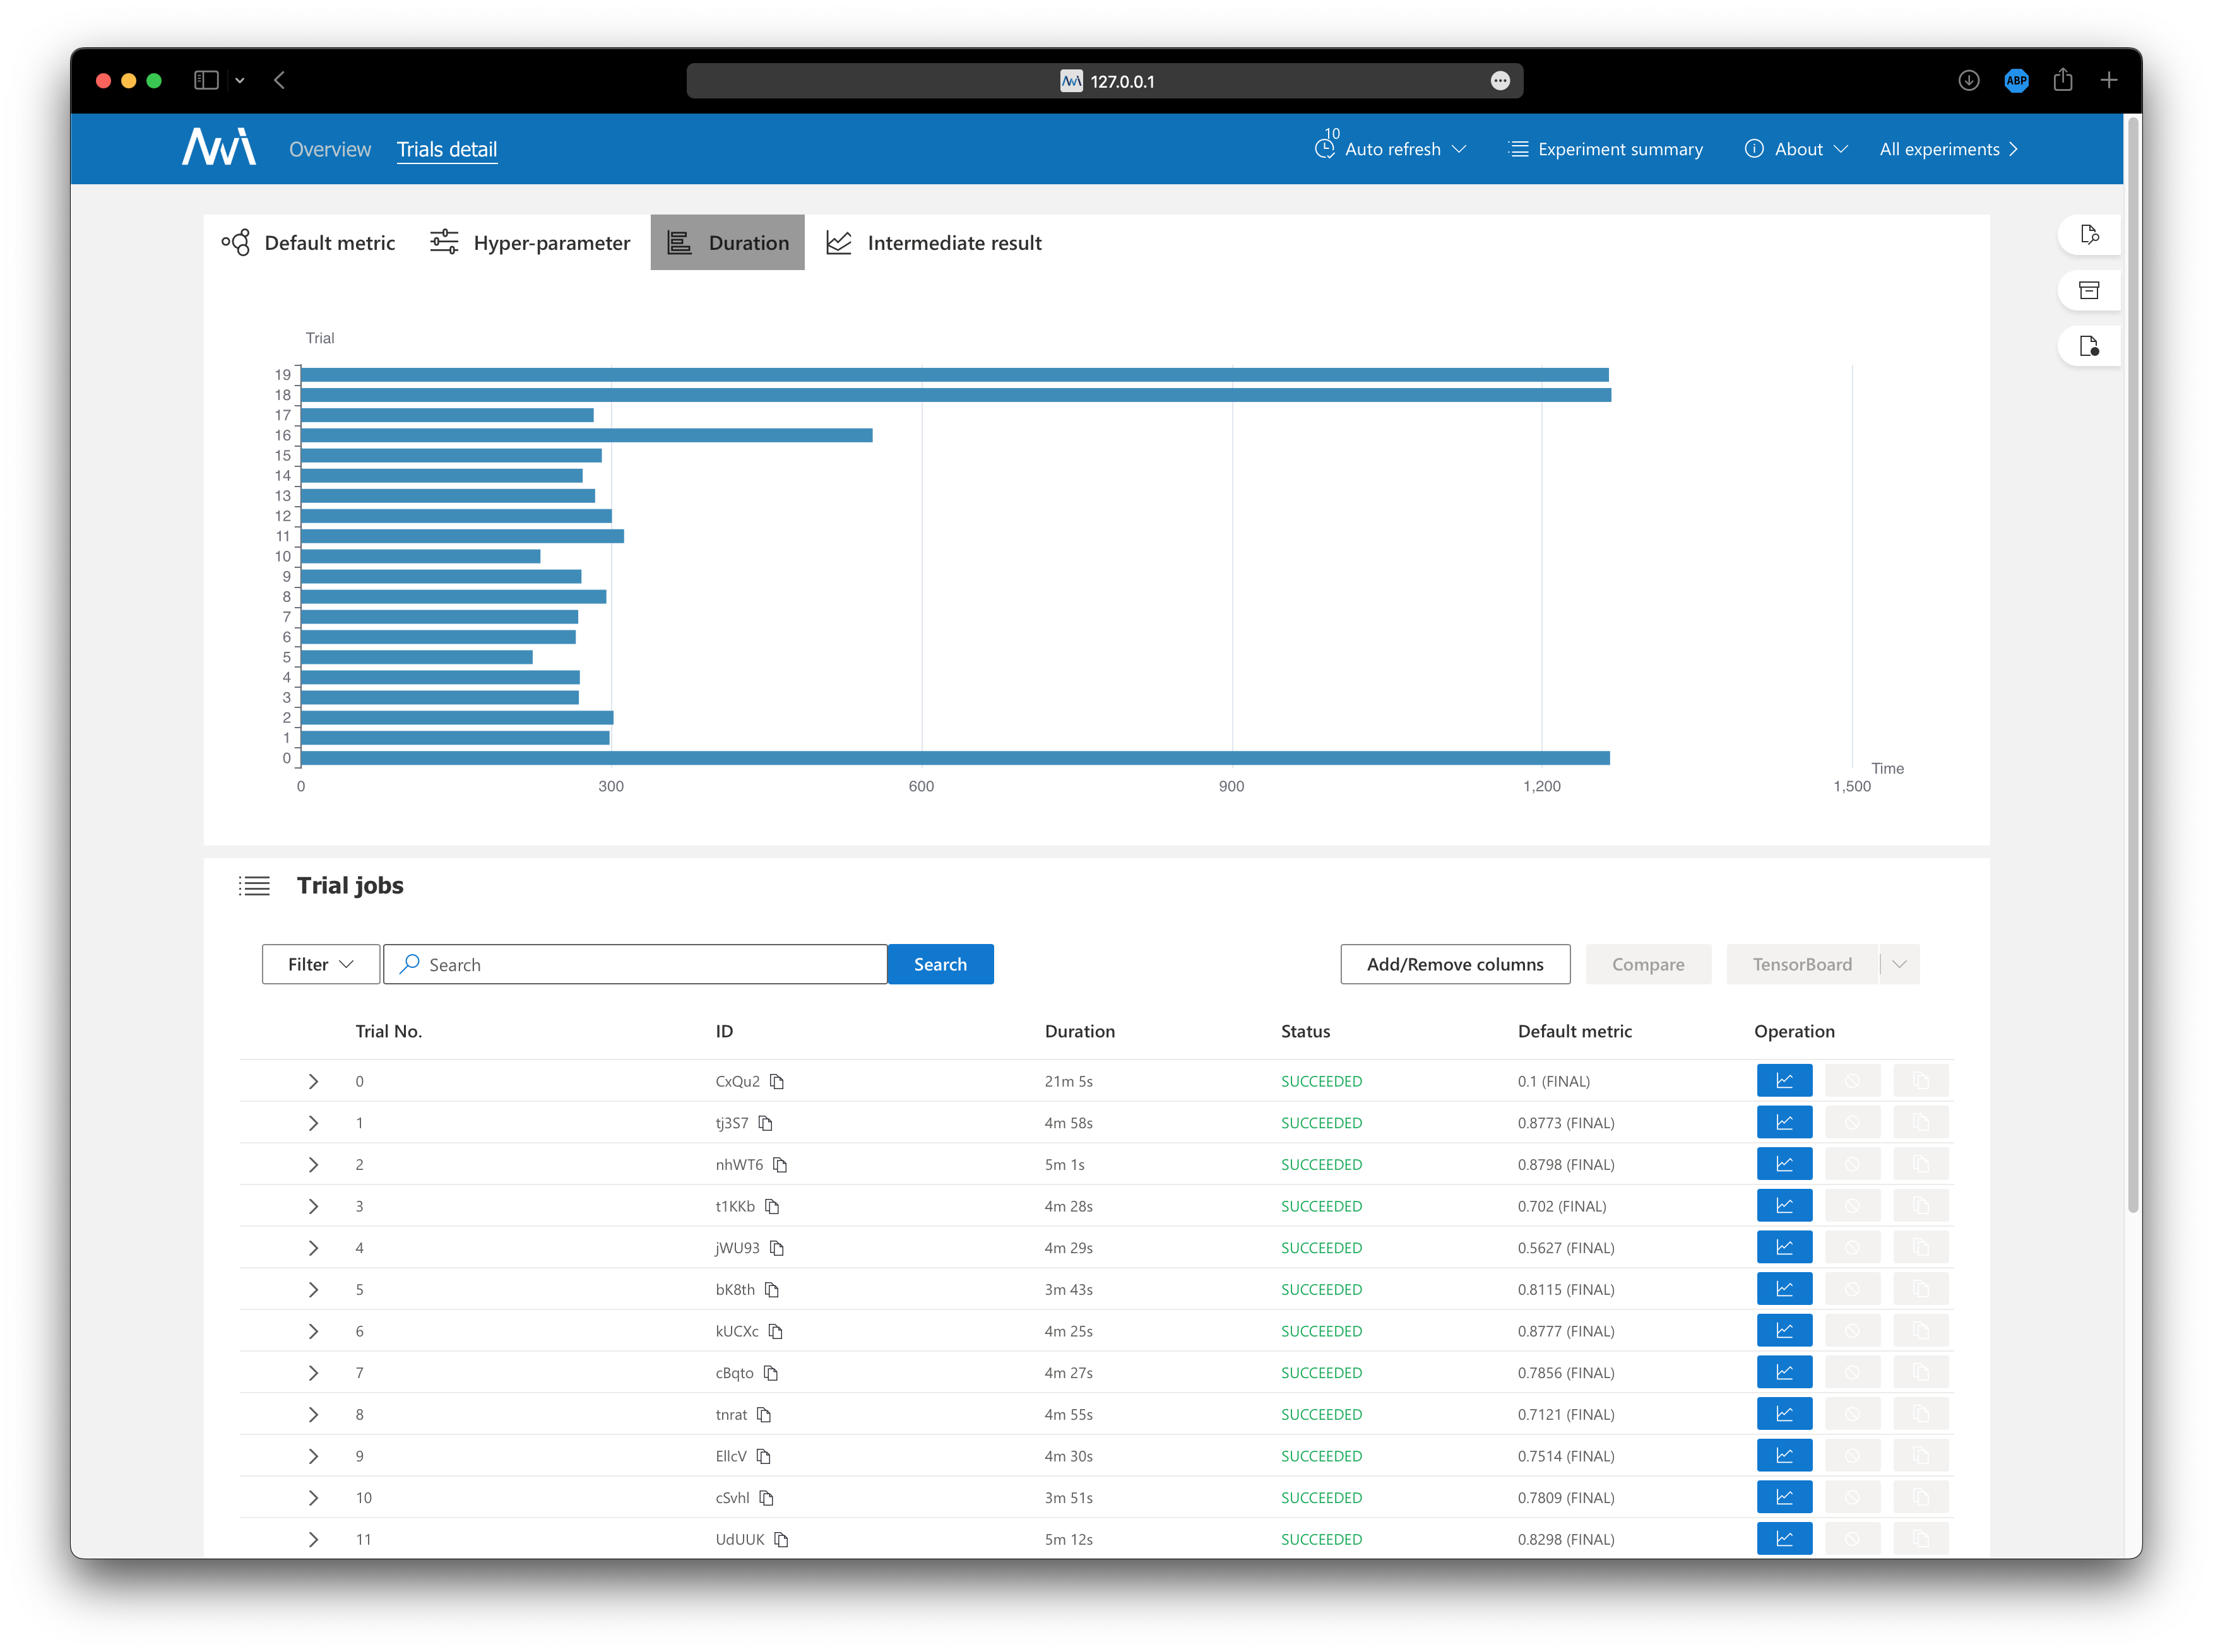
\includegraphics[width=3.5in]{../proj3/figures/mlp_evolution_batch_latency.png}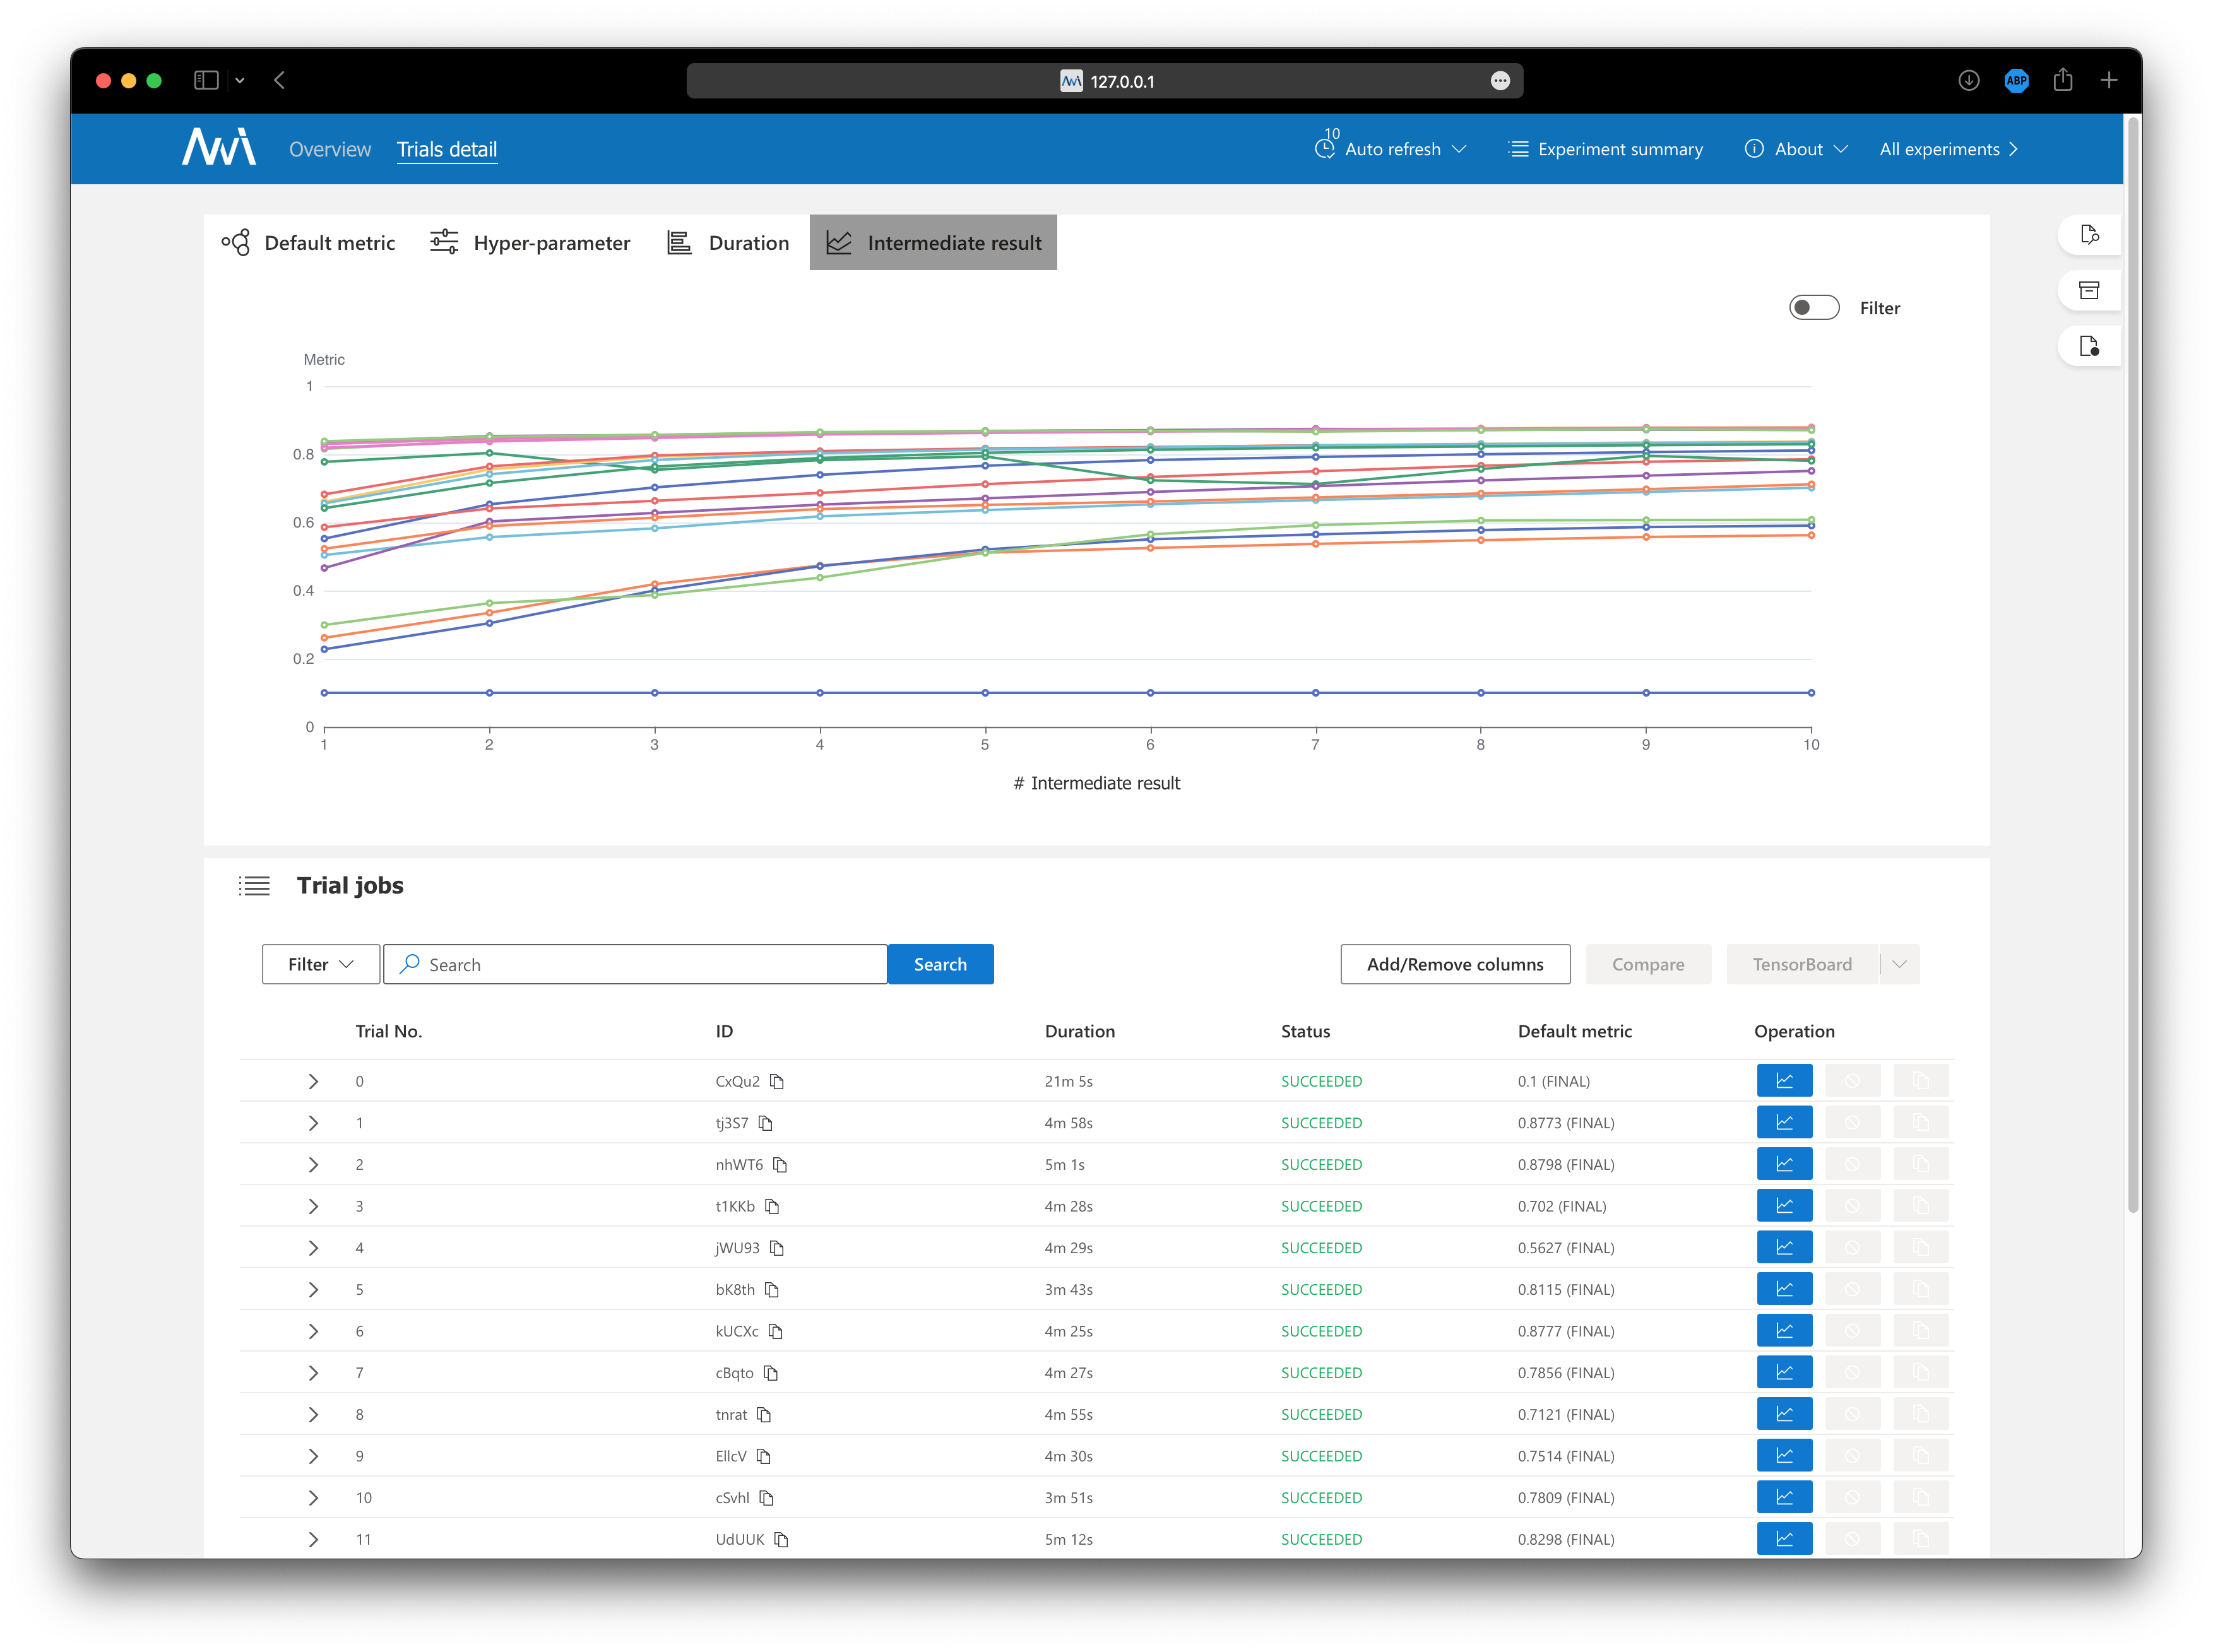
\includegraphics[width=3.5in]{../proj3/figures/mlp_evolution_batch_intermediate.png}}
    \caption{MLP with Evolution Tuner on Learning Rate, Momentum, Feature Size, and Batch Size}
    \label{fig:mlp-evolution-batch}
\end{figure}

Figure \ref{fig:mlp-hyperband-batch} shows the result of the MLP with Evolution. We observe that Trial 6 has the most optimal parameters with a validation accuracy of 88.14\%. The optimal parameters for this trial are a learning rate of $0.0244$ and a momentum of $0.7010$. The optimal batch size is 64 and the number of features is 512. Duration for each trial ranged from 3-33 minutes. Trial 6 had a execution time of 5:01.

\begin{figure}
    \centerline{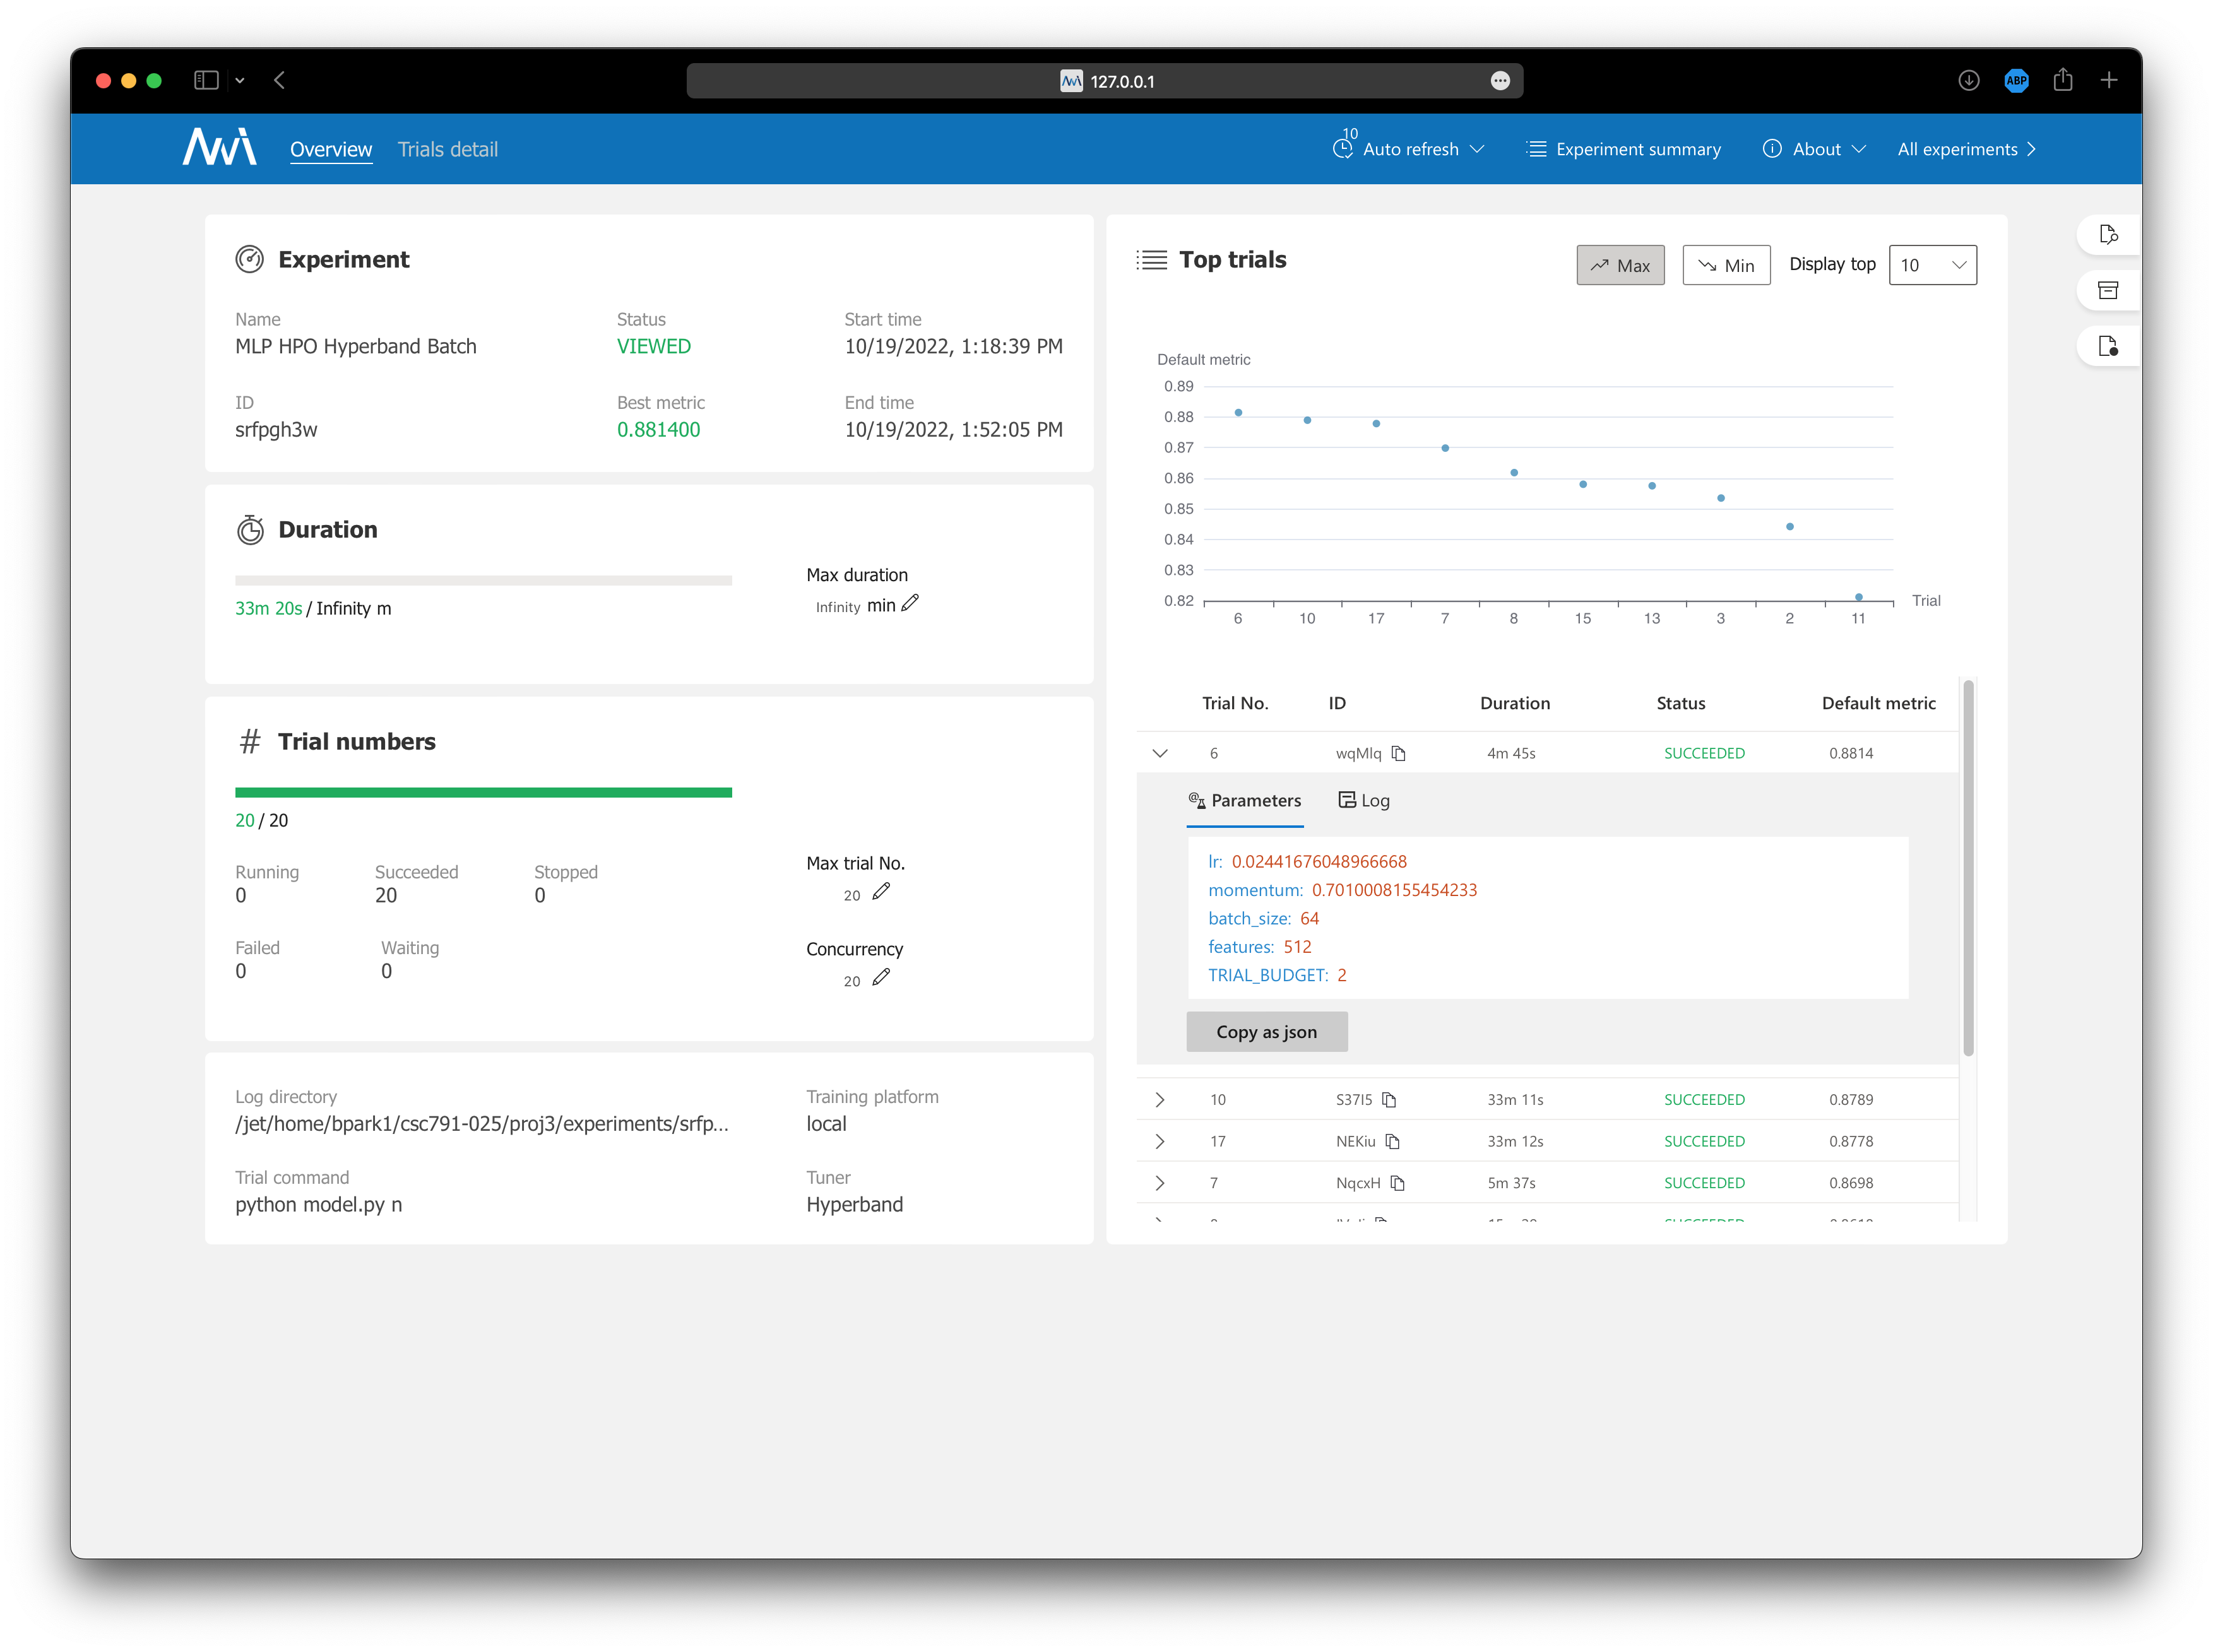
\includegraphics[width=3.5in]{../proj3/figures/mlp_hyperband_batch_overview.png}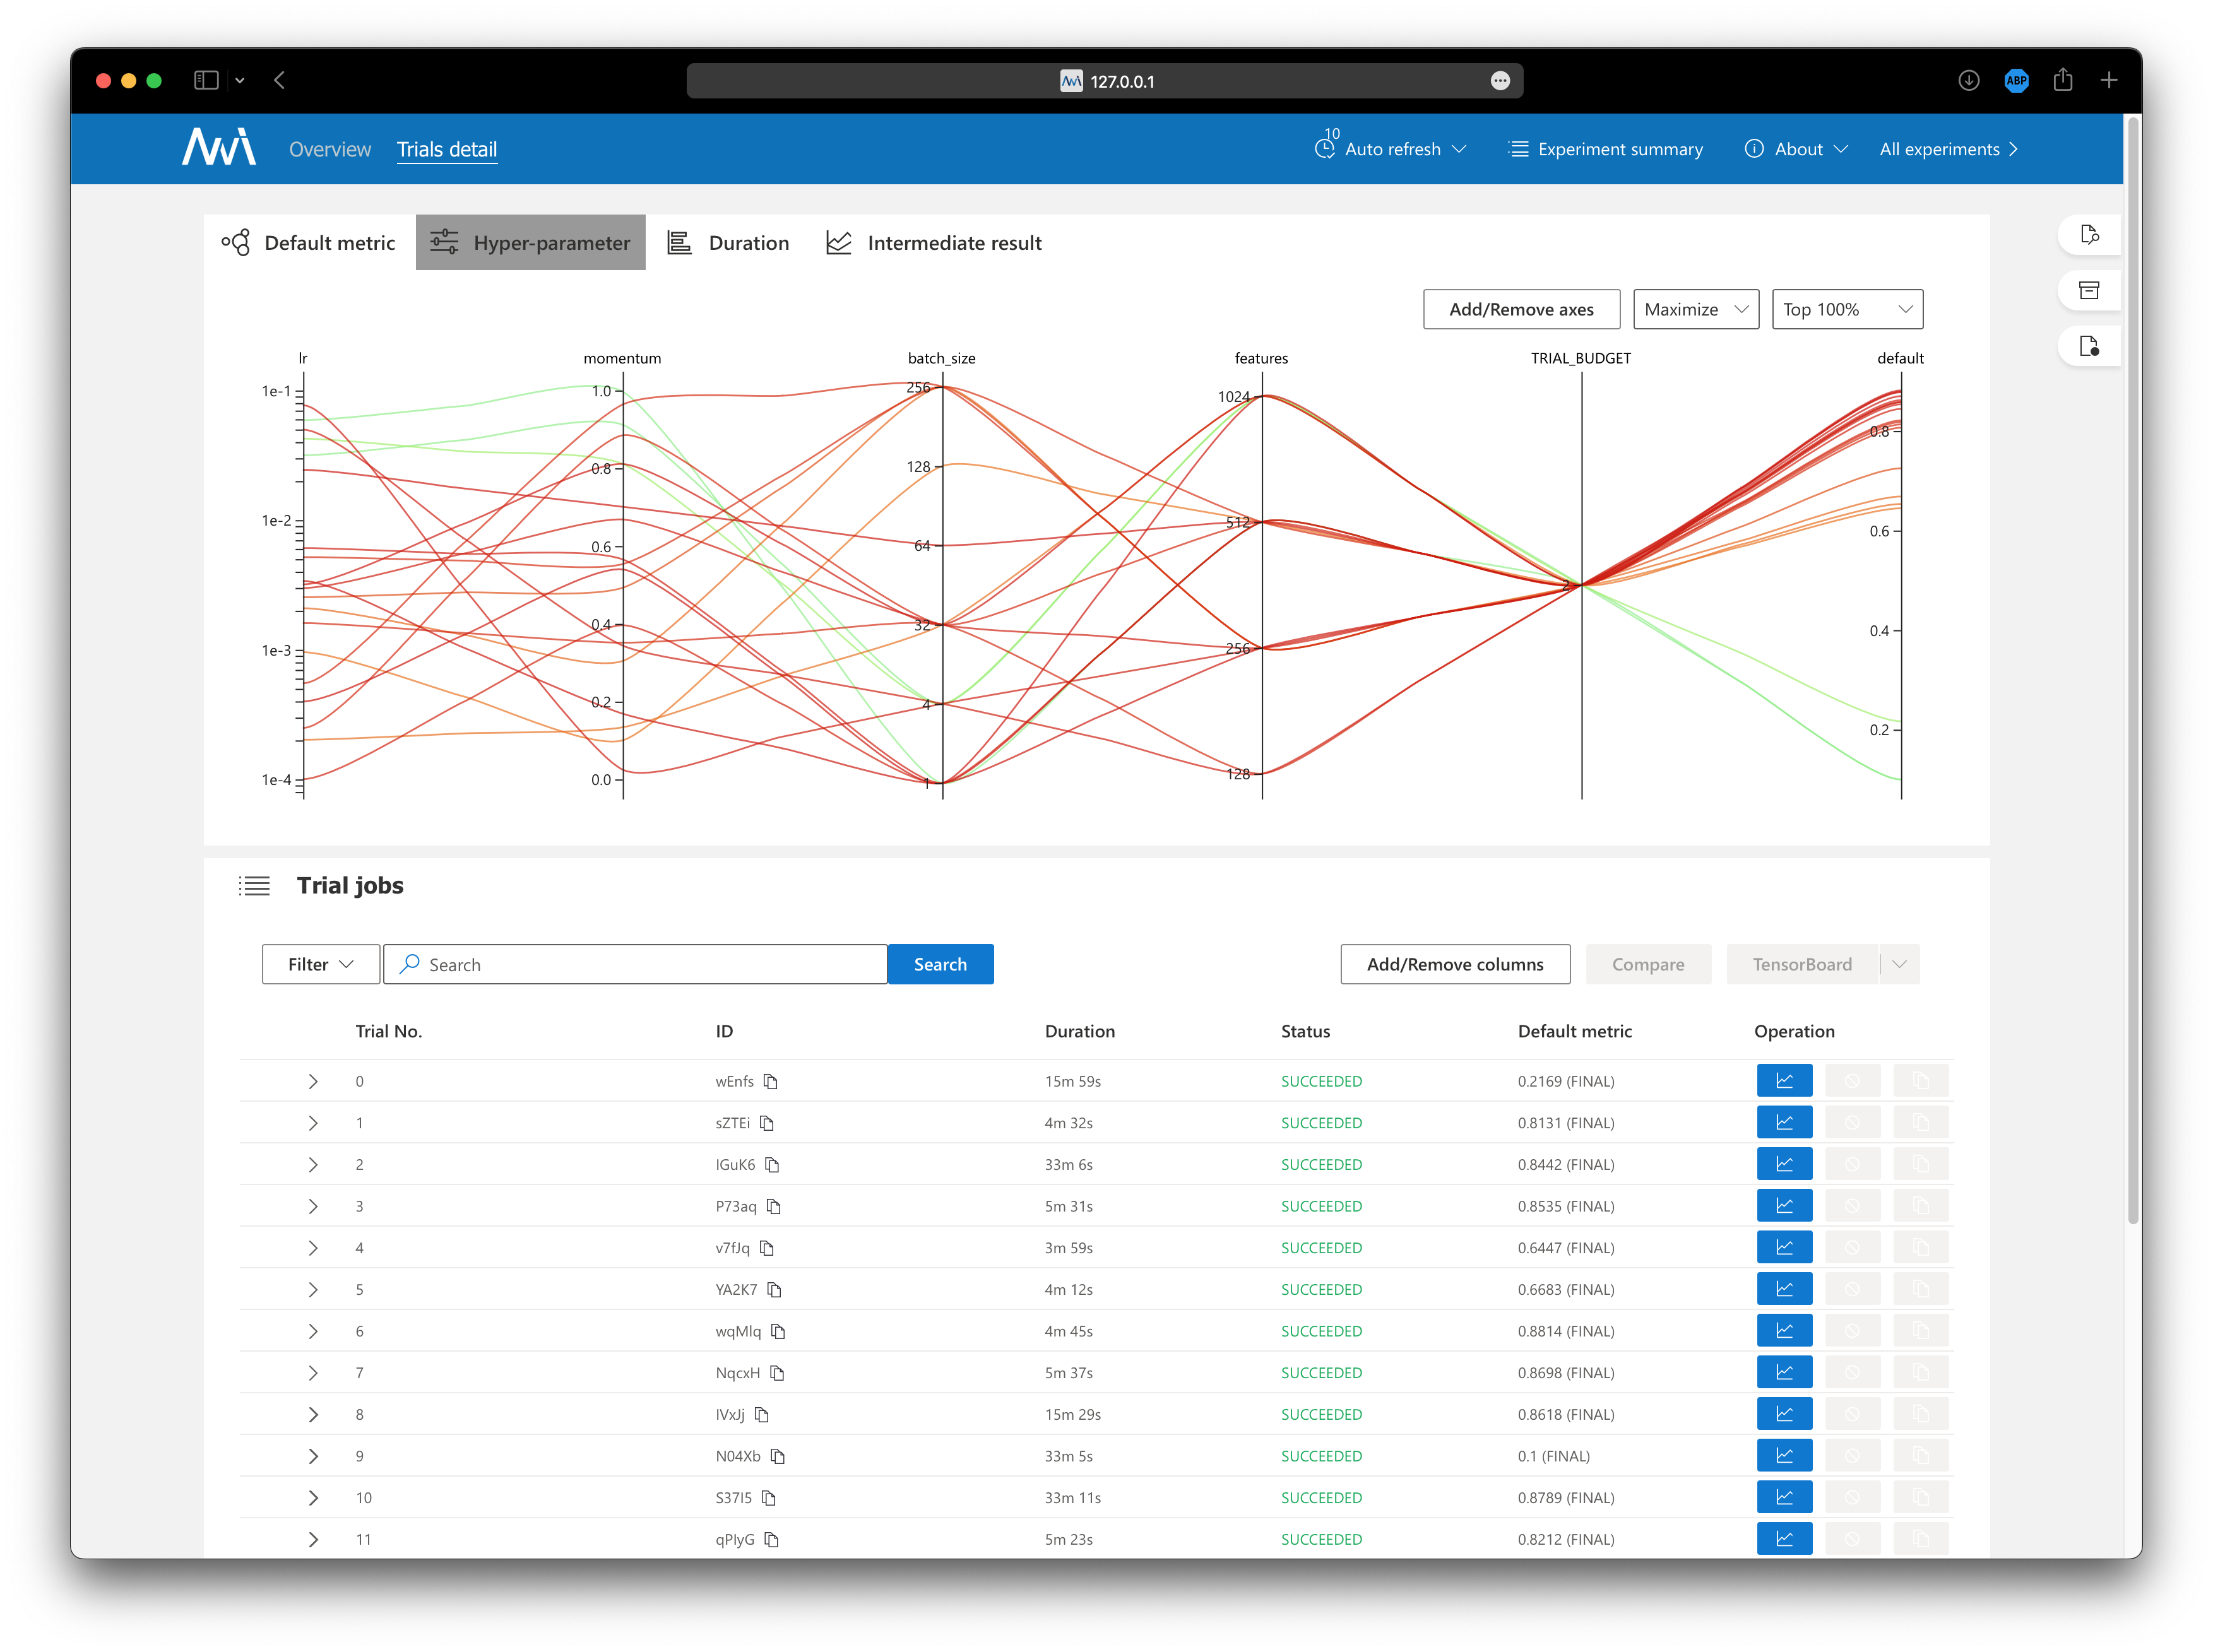
\includegraphics[width=3.5in]{../proj3/figures/mlp_hyperband_batch_hyperparameter.png}}
    \centerline{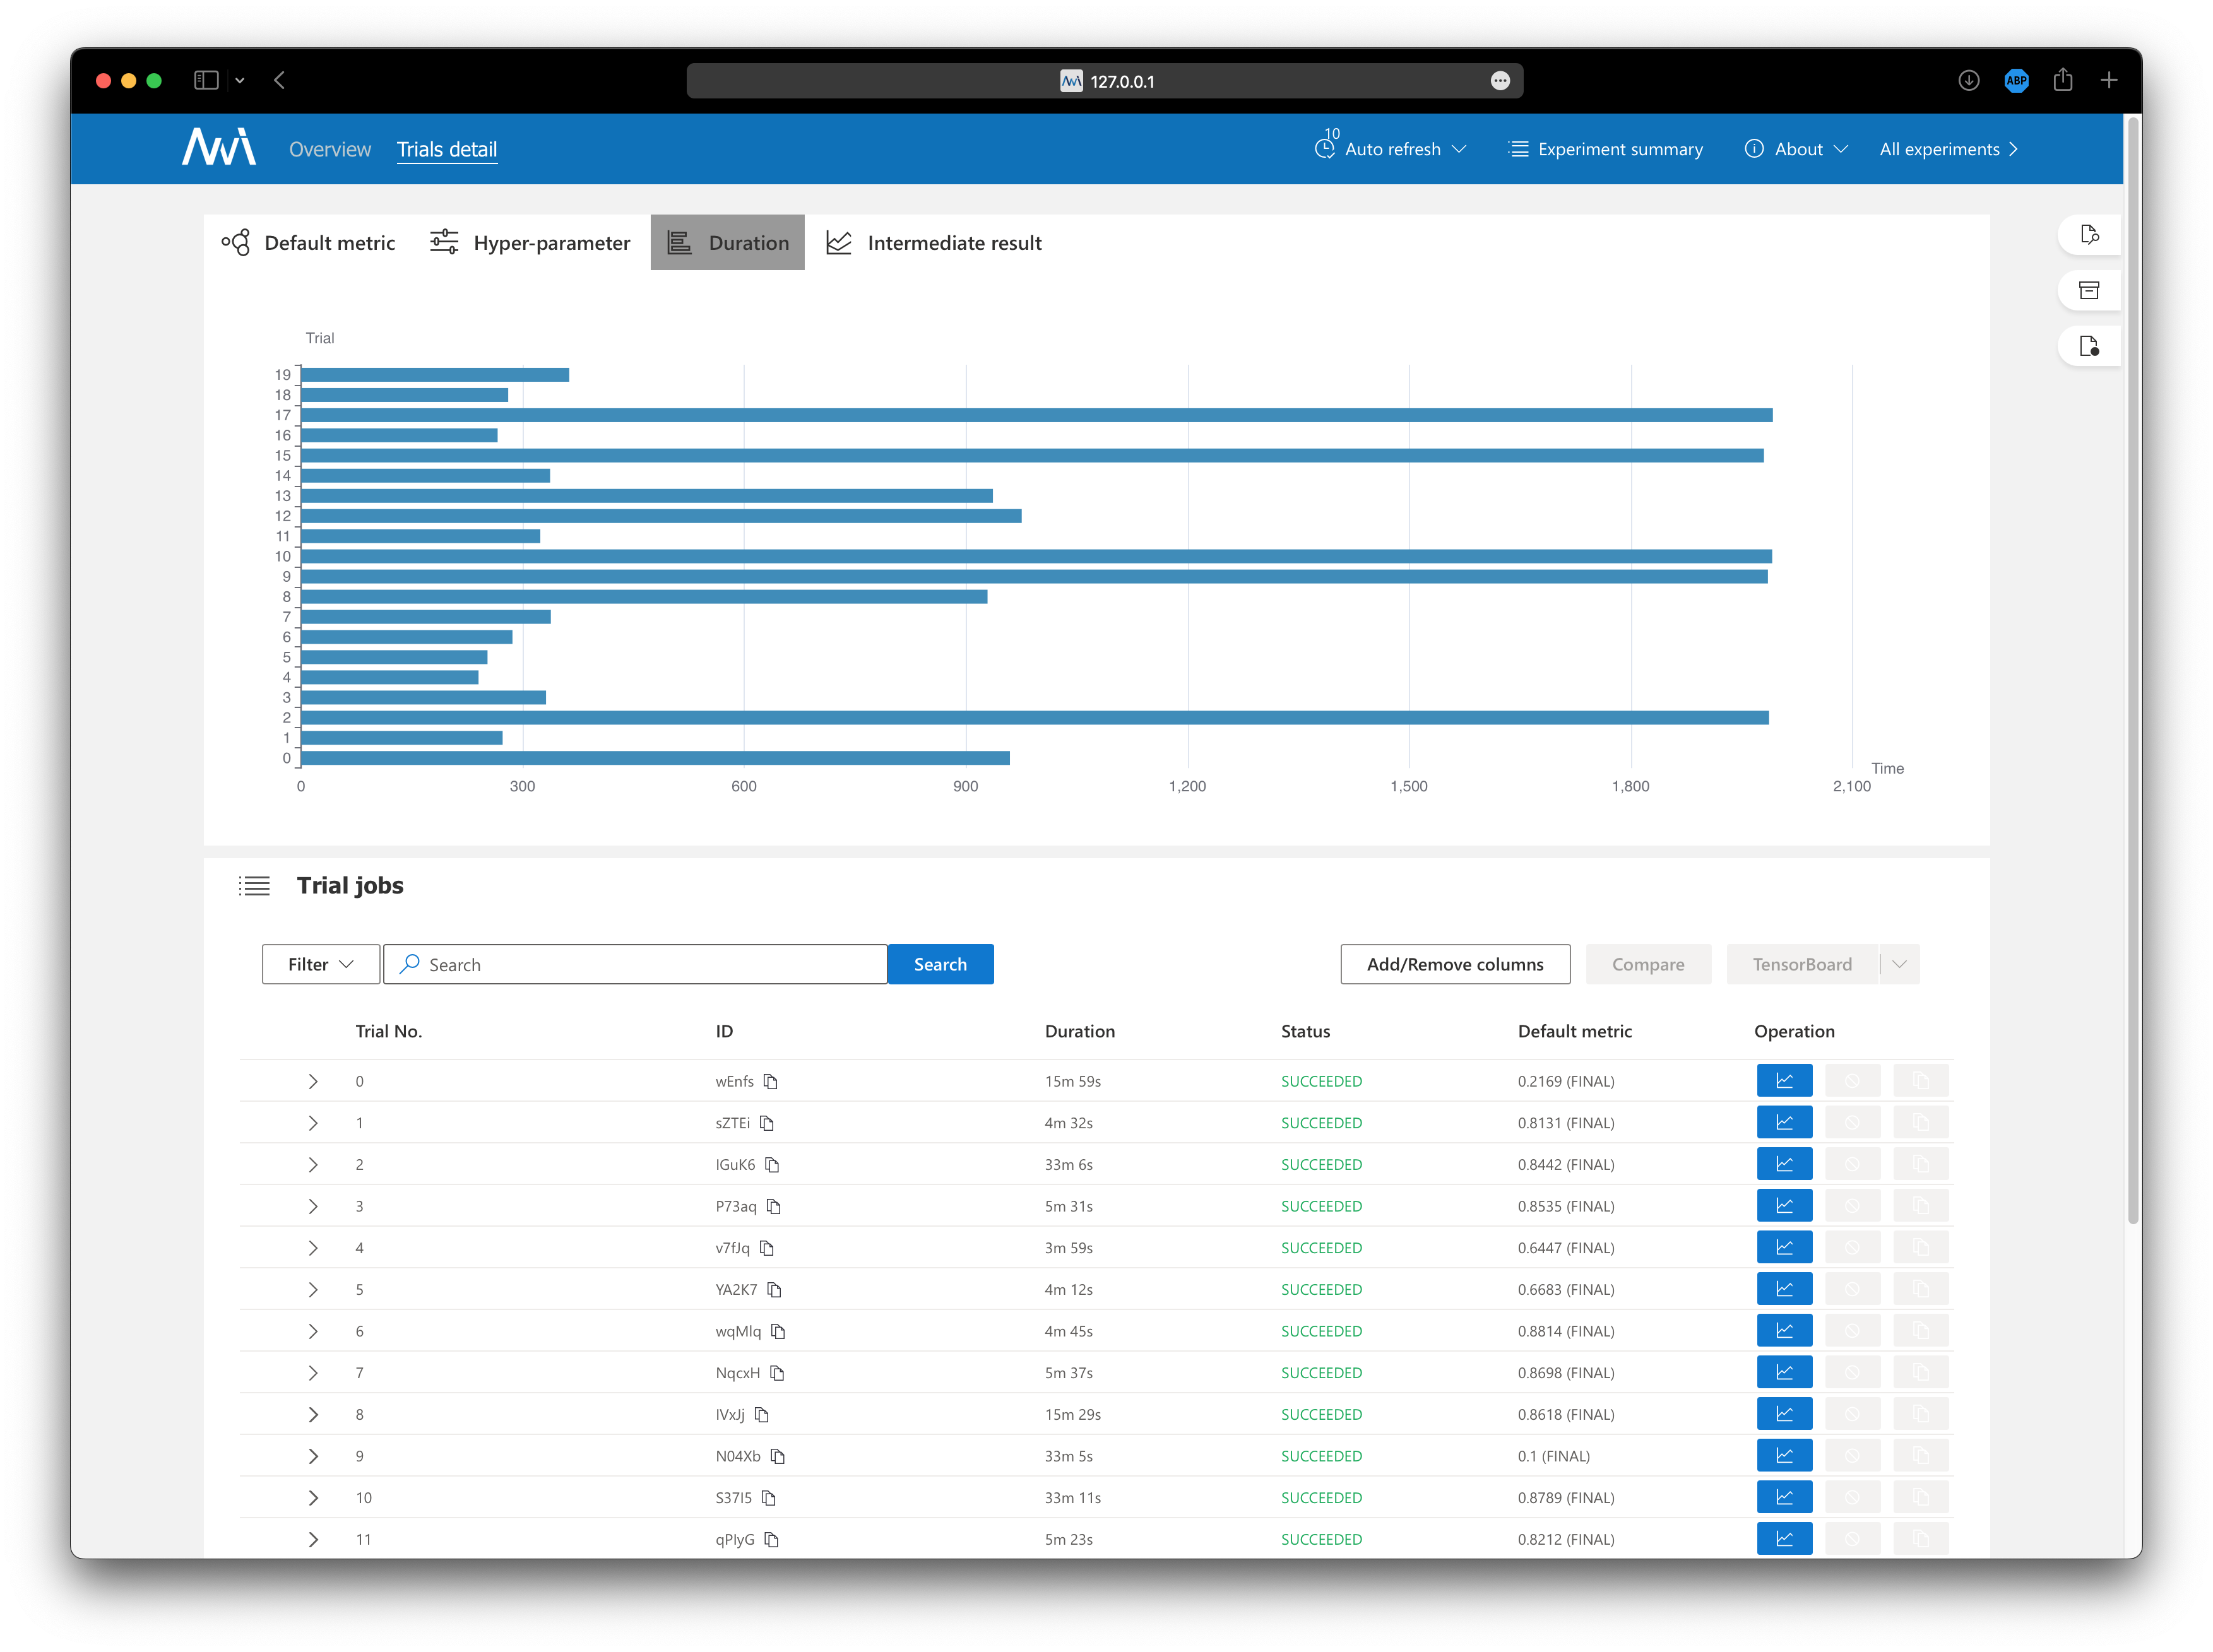
\includegraphics[width=3.5in]{../proj3/figures/mlp_hyperband_batch_latency.png}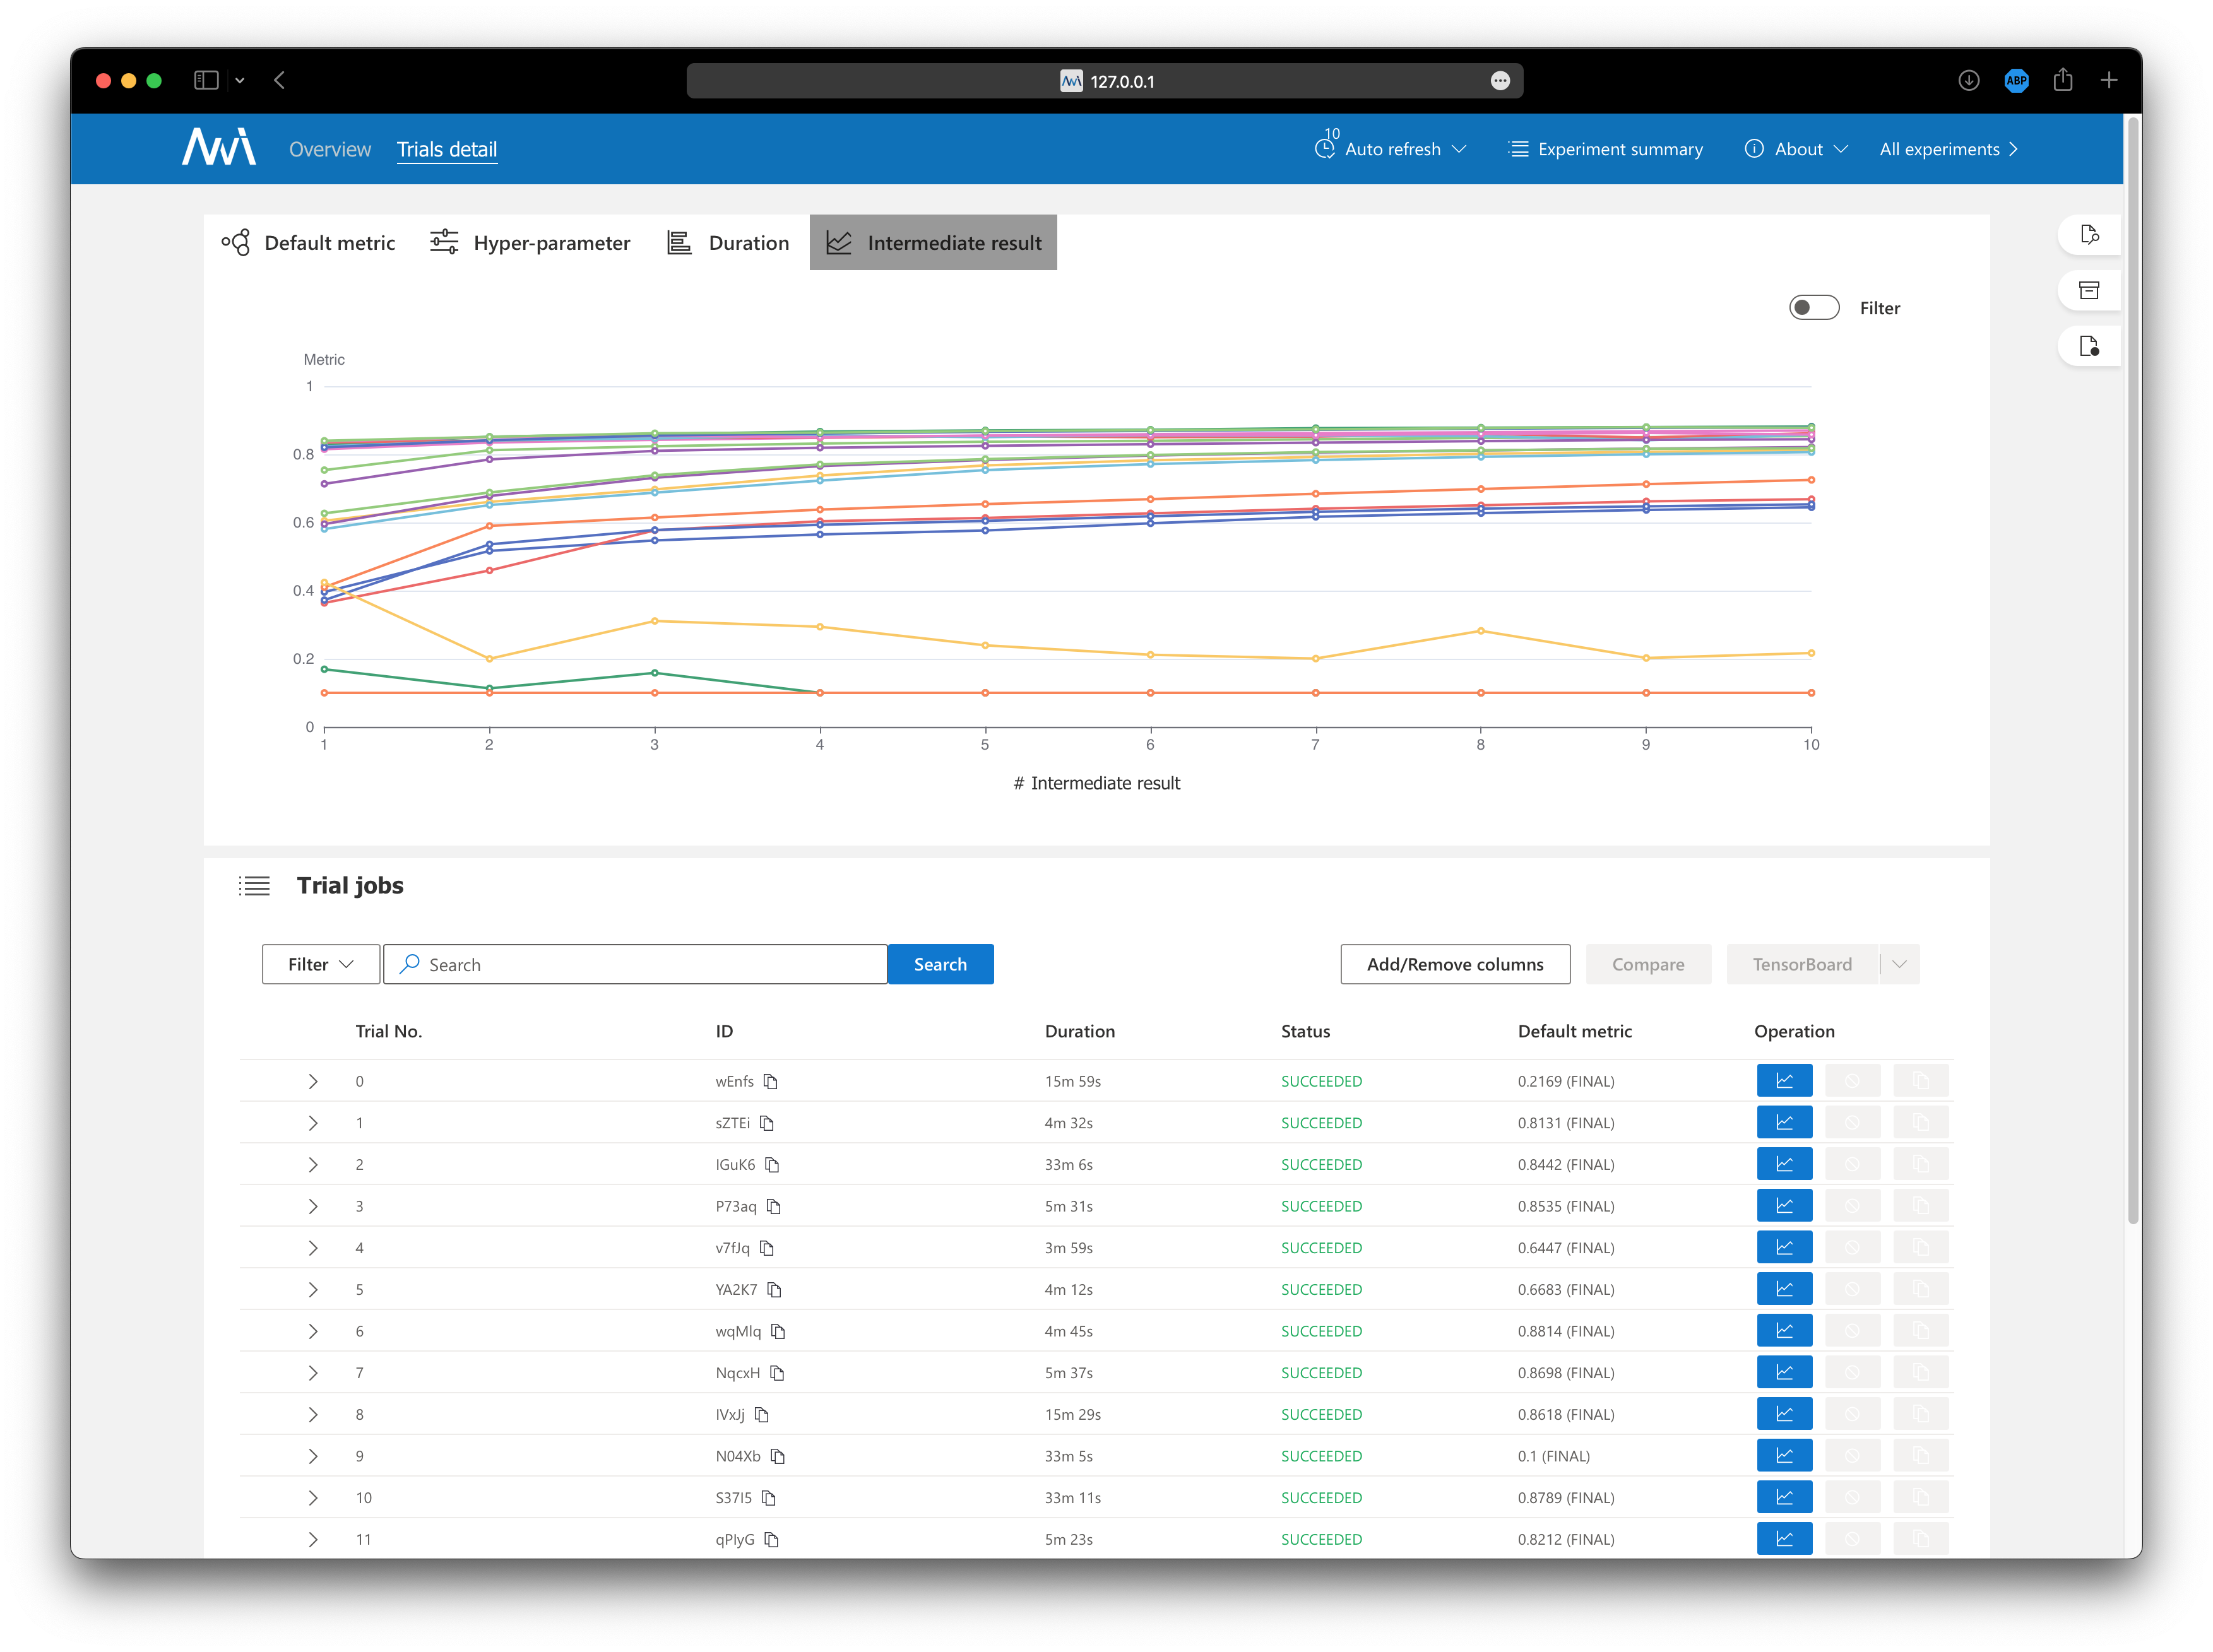
\includegraphics[width=3.5in]{../proj3/figures/mlp_hyperband_batch_intermediate.png}}
    \caption{MLP with Hyperband Tuner on Learning Rate, Momentum, Feature Size, and Batch Size}
    \label{fig:mlp-hyperband-batch}
\end{figure}

For all of the tuners, we are able to see speed differences now. TPE still performs the best, but it has a larger batch size than the others. It also has a longer time, which doesn't intuitively make sense.

\subsection{VGG-19 HPO Experiments with Learning Rate and Momentum}
Just in case MLP didn't show interesting results, we also ran a few hyperparameter tuners for VGG-19. We couldn't run the whole suite of configurations as it took very long, so we capped our trials at 5 hours. Figure \ref{fig:vgg-all} shows a overall view of our results. Hyperband HPO tuner could not finish, so their results could've been better if ran to completion for a fair evaluation. Evolution HPO tuner had the best hyperparameters with a validation accuracy of 76.15\%. We actually crashed our initial run, because it hit OOM. Lowering down the concurrency from 20 to 5 resolved this issue, as VGG-19 is a much larger model and the NVIDIA V100 has only 32GB of HBM memory.

\begin{figure}
    \centerline{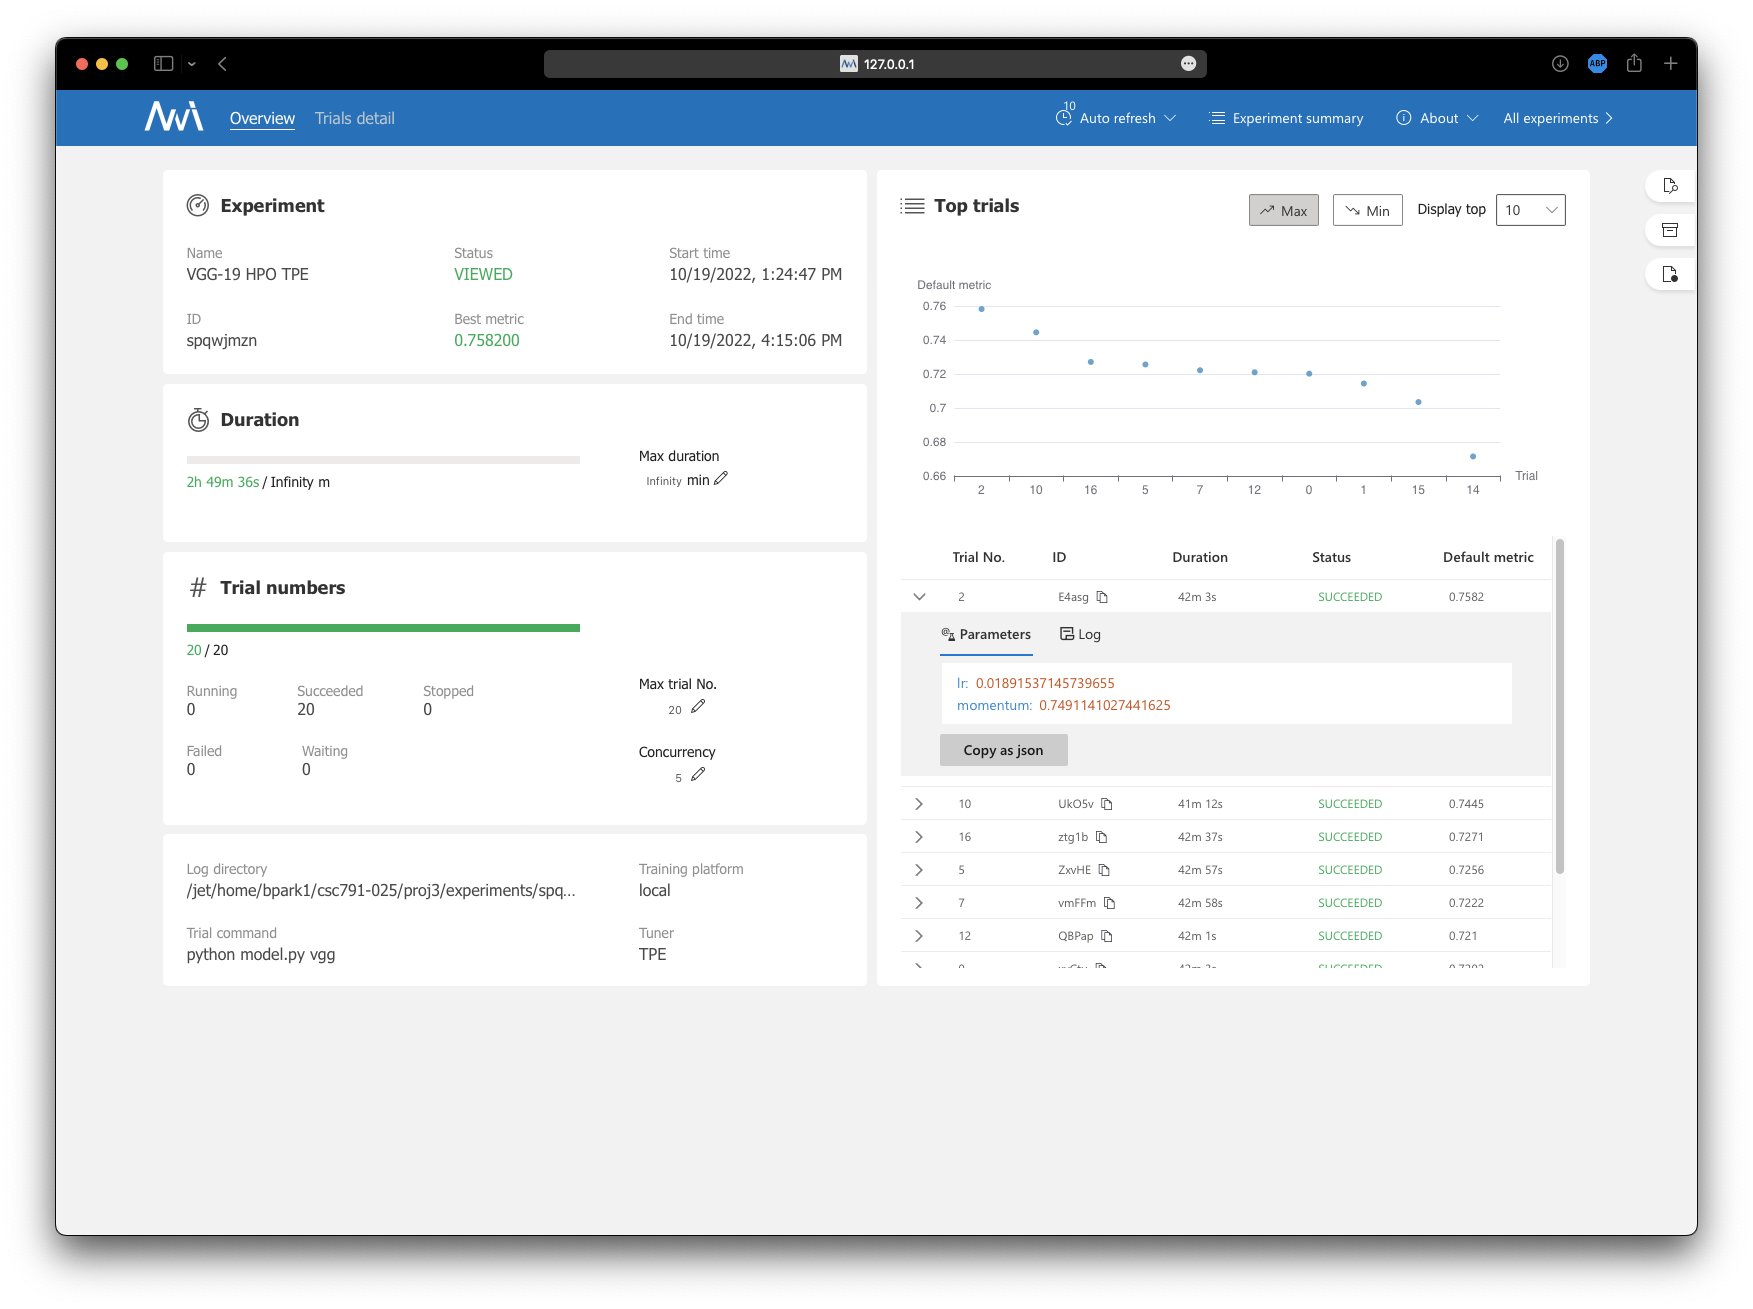
\includegraphics[width=3.5in]{../proj3/figures/vgg_tpe_overview.png}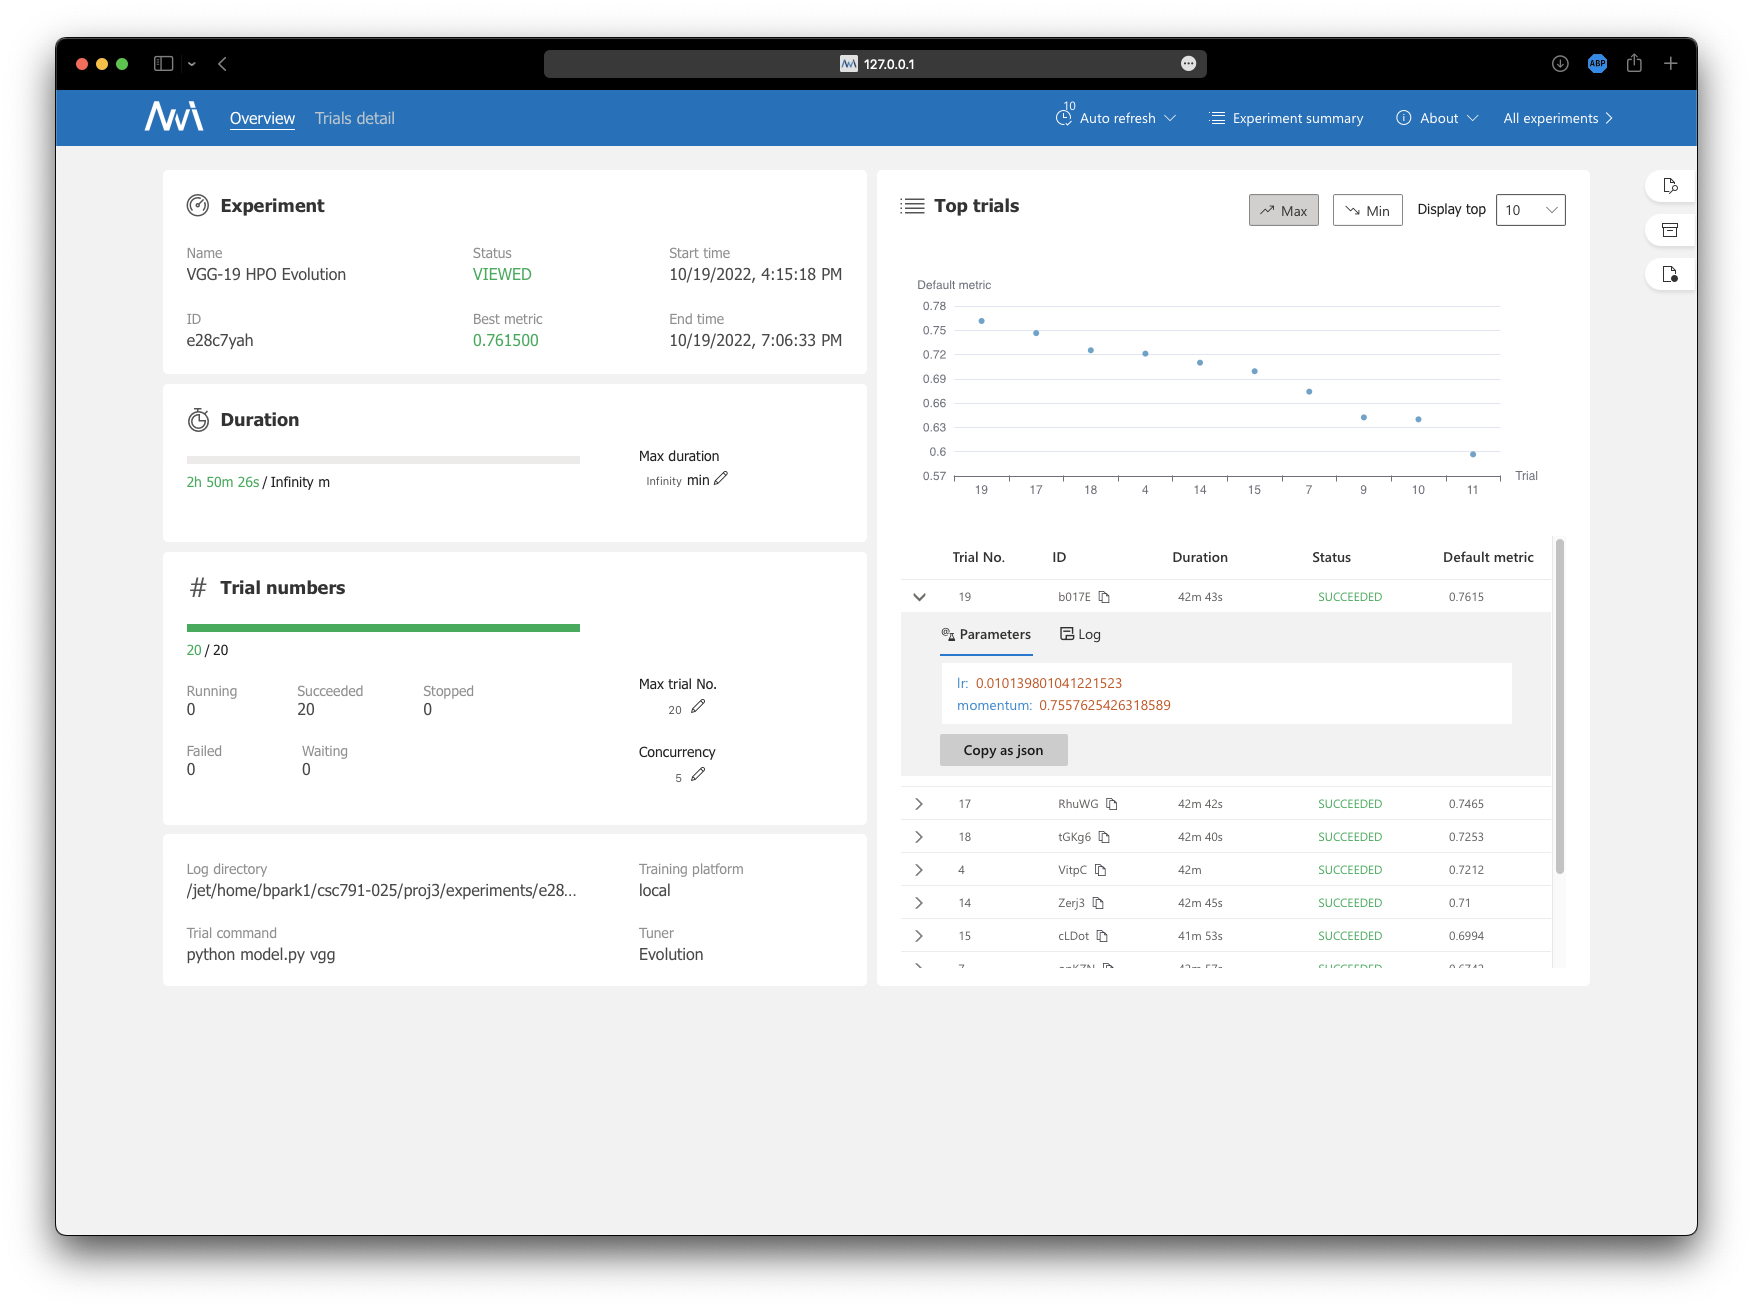
\includegraphics[width=3.5in]{../proj3/figures/vgg_evolution_overview.png}}
    \centerline{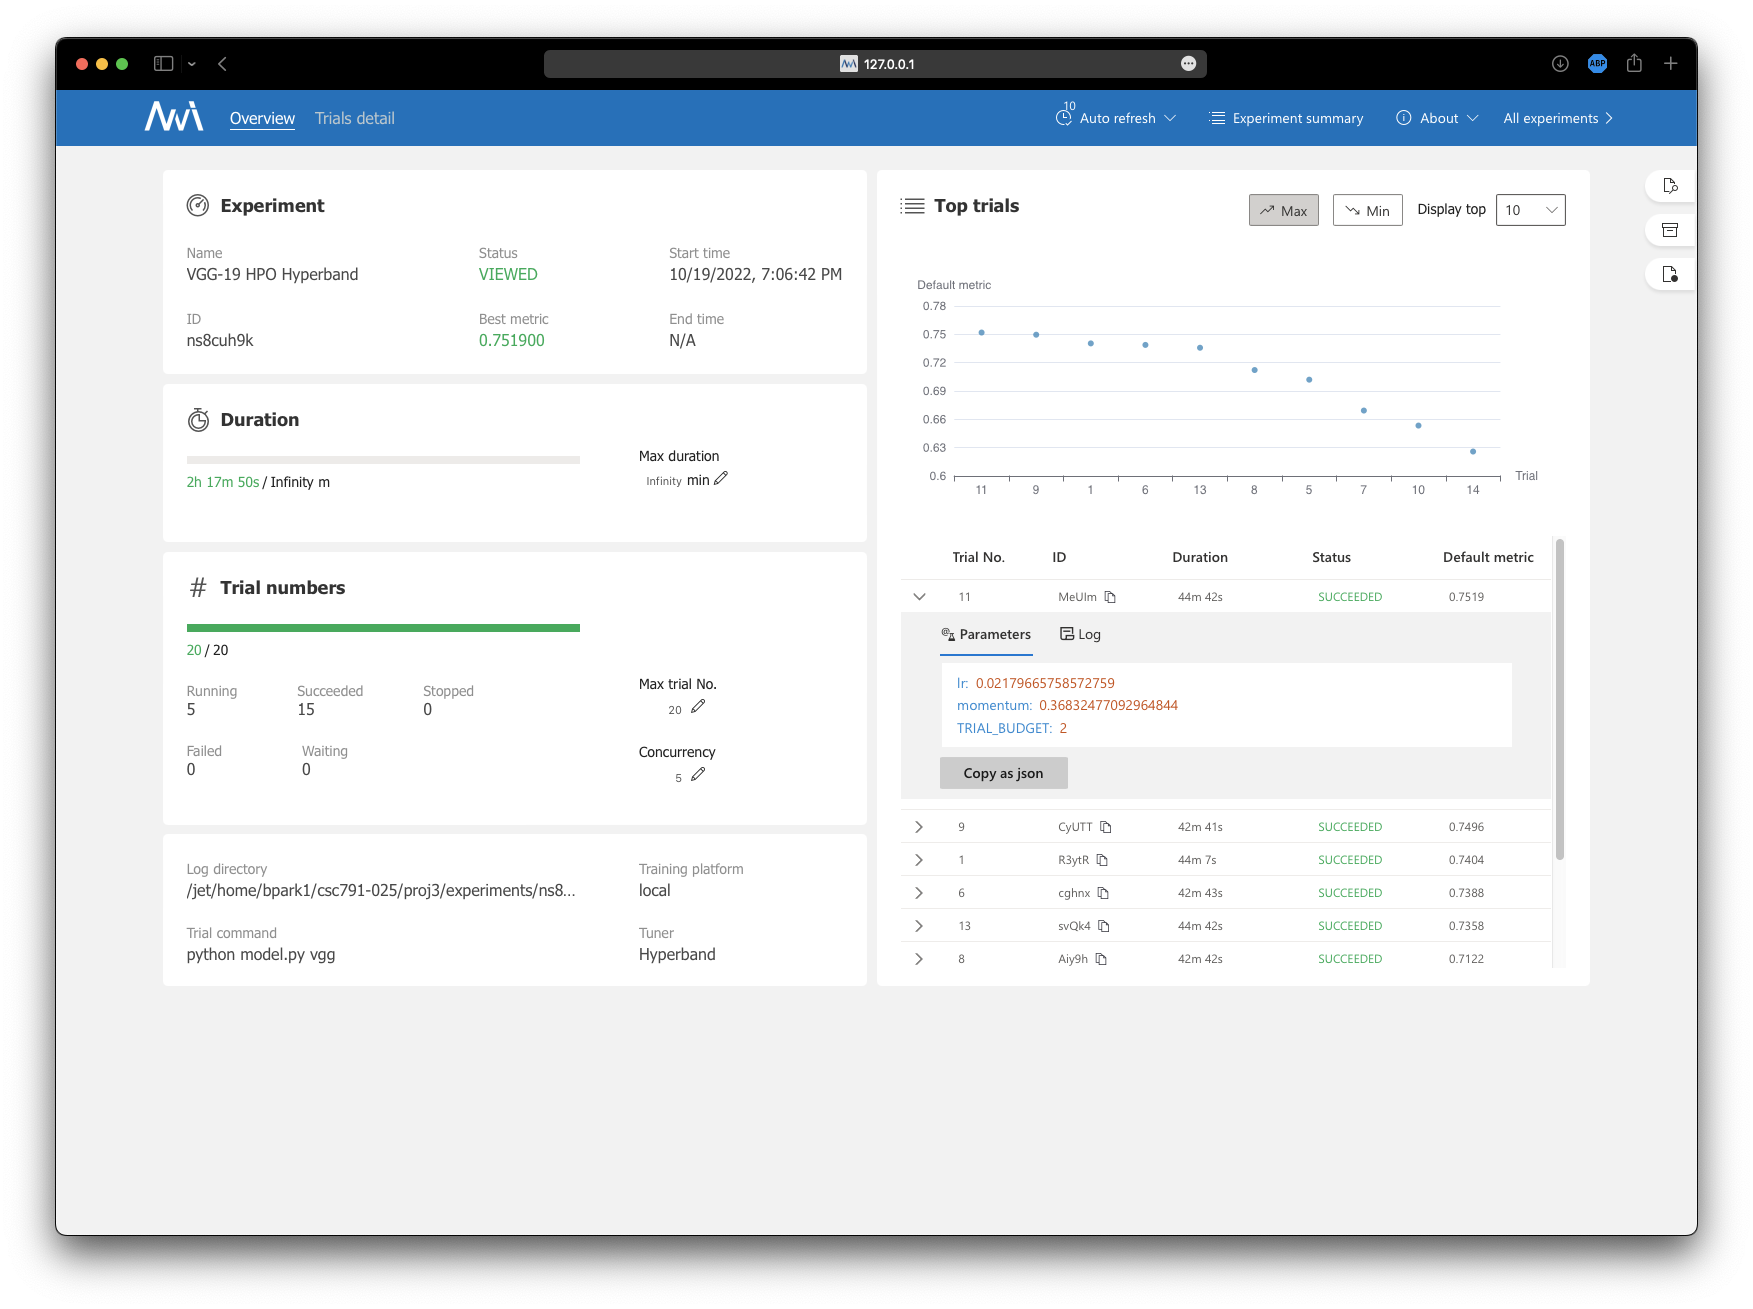
\includegraphics[width=3.5in]{../proj3/figures/vgg_hyperband_overview.png}}
    \caption{VGG HPOs on Learning Rate and Momentum}
    \label{fig:vgg-all}
\end{figure}

\section{Lessons Learned}
%(4) What lessons you have learned through the project.
NNI fortunately parallelizes the hyperparameter tuning process by enabling concurrent models to be trained at the same time. Unfortunately, we weren't aware of this when switching between hardware when running experiments. Thus we often crashed our own devices or had our devices struggle to operate due to a configuration suited towards high end GPU like the V100. 

There are actually many competing hyperparameter optimizers and tuners out there that we were aware of. PyTorch presents Ray Tune in their \href{https://pytorch.org/tutorials/beginner/hyperparameter_tuning_tutorial.html}{documentation} as a recommendation for hyperparameter tuning \cite{ray-tune}. There is also an \href{https://github.com/microsoft/nni/issues/1743}{issue and discussion} about what the differences between the two are, which is positioning. I think the main difference is that NNI is a platform that also eases for other methods like pruning and quantization. So much more hyperparameter tuning frameworks exist like HyperOpt, sklearn's GridSearchCV, Optune, Weights \& Biases, and many more \cite{optuna}. Some support classical machine learning algorithms, and other can support deep neural networks. But in the end, the tools seem to all serve a similar purpose with different positioning.

\section{GitHub Repository}
%(5) A link to your github repository that contains all the scripts used in this project and a README describing the structure of the repository and how the folders in the repository correspond to the items in the report. The report must be in PDF, with the five required parts clearly marked. 
The GitHub repository for this report is publicly accessible here \cite{proj3-repo}. To reproduce our findings, please read the \verb|README.md| under the \verb|proj3| directory. If there are any setup issues on bridges-2 supercomputer or locally, please contact \href{mailto:bcpark@ncsu.edu}{bcpark@ncsu.edu}.

\bibliographystyle{ieeetr}
\bibliography{references}

\end{document}
